\documentclass[10pt,doublespacing,edeposit]{uiucthesis2020}
%draftthesis

% {{{ packages

\usepackage{blindtext}
\usepackage{cite}
\usepackage{array}
\usepackage{booktabs}
\usepackage{xcolor}
\usepackage{comment}
\usepackage{textcomp}
\usepackage{inputenc}
\usepackage{upgreek}
\usepackage{wrapfig}
\usepackage[margin=1in]{geometry}
\usepackage{multirow}
\usepackage{subcaption}
\usepackage{color}
\usepackage{makecell}
\usepackage{mathtools}
\usepackage{soul}
\usepackage{placeins}
\usepackage{flafter}
\usepackage{rotating}

% math
\usepackage{fixmath}
\usepackage{amsmath}
\usepackage{amsthm}
\usepackage{amssymb}
\usepackage{stmaryrd}

% pretty links
\usepackage{xparse}
\usepackage{hyperref}
\usepackage{cleveref}
\usepackage{graphicx}
\hypersetup{
    colorlinks=true,
    urlcolor=blue,
    citecolor=black,
    linkcolor=black
}

% better environments
\usepackage[shortlabels]{enumitem}
\usepackage{booktabs}

% fancier font
\usepackage[sc]{mathpazo}
% better typography
\usepackage[activate={true,nocompatibility}, % activate protrusion and font expansion
            final,              % enable microtype, use draft to disable
            tracking=true,
            kerning=true,       % optimise interactions between characters
            spacing=true,       % more uniform spacing between words
            factor=1100,        % more protrusion
            stretch=10,         % smaller values (default 20, 20) to avoid blurring
            shrink=10]{microtype}
\microtypecontext{spacing=nonfrench}
\SetTracking{encoding={*}, shape=sc}{40}

% }}}

% {{{ commands

\NewDocumentCommand \dx { O{x} } {\,\mathrm{d} #1}
\NewDocumentCommand \vect { m } { \mathbold{#1} }
\NewDocumentCommand \jump { m } { \left\llbracket #1 \right\rrbracket }
\NewDocumentCommand \avg { m } { \left\langle #1 \right\rangle}
\NewDocumentCommand \od { m m } { \dfrac{\mathrm{d} #1}{\mathrm{d} #2} }
\NewDocumentCommand \pd { m m } { \dfrac{\partial #1}{\partial #2} }

\newcommand*{\cumnas}{Cu$_{0.82}$Mn$_{1.18}$As}

% }}}

% {{{ title

\title{Magnetic ordering and spin wave dynamics in transition metal arsenides}
\author{Manohar H. Karigerasi}
\department{Materials Science and Engineering}

\schools{
B. Tech., Indian Institute of Technology Roorkee, 2016 \\
M. S., University of Illinois at Urbana-Champaign, 2017
}

\phdthesis
\advisor{Daniel P. Shoemaker}
\degreeyear{2021}

\committee{
Associate Professor Daniel P. Shoemaker, Chair \\
Professor David G. Cahill \\
Professor Jian-Min Zuo \\
Research Assistant Professor Gregory MacDougall \\
}

% }}}

\begin{document}

\maketitle

% {{{ front matter

\begin{frontmatter}

\begin{abstract}
Metallic antiferromagnets have gained interest in recent times due to the possibility of being useful as a memory device. Arsenic forms a large pool of magnetic metals in combination with other transition metals that have largely been ignored so far. In this report, we discover a new ternary metallic arsenide in the Cu-Mn-As phase space, identify its chemical and magnetic structure, and characterize its electrical and magnetic properties. We also carry out the magnetic structure refinement of Mn$_3$As$_2$ from neutron powder diffraction data at different temperatures to understand the magnetic ordering in Mn-As compounds. Using inelastic neutron scattering measurements, we determine exchange interactions in Fe$_2$As, which has the same structure as CuMnAs, showing a highly 2D magnon character although the phonons are 3D. Finally, we report a magnetic-structural coupled transition across 300 K in tetragonal CuMnAs and determine the correct magnetic structure of the compound.
\end{abstract}

\chapter*{Acknowledgments}

This project would not be possible without many people. Firstly, thanks to my advisor, Prof. Daniel P. Shoemaker.

%\begin{dedication}
%To Coffee
%\end{dedication}

\tableofcontents
\listoftables
\listoffigures

\end{frontmatter}

% }}}

% {{{ main matter

\begin{mainmatter}

%##################chapter 1
\chapter{Introduction}

\section{Magnetic information storage}

% Information 
In information memory storage devices, there is typically a trade-off between the optimum speed or response time and the complexity and size of memory storage \cite{Wing1986}. Volatile memory refers to temporary memory storage where the data is lost when the power is removed. Volatile memory such as SRAM (static random access memory) and DRAM (dynamic random access memory) are used as CPU caches and main memory respectively. SRAM has much faster access times and does not require periodic refreshing. However, it requires four to six transistors per bit as compared to one transistor and one capacitor in DRAM devices \cite{Meena2014}. Non-volatile memory (NVM) storage devices on the other hand, retain their data for a long period of time until perturbed. Modern computers mostly use flash memory based solid state drives (SSD) and magnetic hard disk drives (HDD) for storing large amounts of data permanently \cite{Meena2014}. The first HDD was invented in 1956 by IBM and since then, has seen more than eight orders of magnitude improvement in the storage density. However, the trilemma in magnetic recording between poor thermal stability, coercive fields and signal-to-noise ratio has resulted in the HDD reaching a saturation limit in their device performance \cite{Krishnan2016}. Flash memory uses floating gate MOSFETs (metal oxide semiconductor field effect transistors) to store memory and does not contain any moving parts. Although SSD have dominated the NVM marketshare last few years, there is an increasing need for alternative NVM technologies that are fast, low power consuming and have high storage density \cite{Meena2014}.

% Emerging NVM
One such emerging NVM is MRAM (magnetoresistive random access memory). Unlike flash memory which uses electronic charge as a medium of memory storage, MRAM uses the electronic spin degree of freedom to store information. Unlike charge based storage devices, MRAM is stable against perturbations such as ionizing radiation \cite{Wadley2016}. MRAM devices consist of cells with magnetic tunnel junctions (MTJ) that have two ferromagnet (FM) layers separated by an insulating layer. One of the layer is pinned where the magnetization orientation is fixed and acts as a reference layer. Depending on the orientation of the free layer, the tunneling magnetoresistance (TMR) is high or low and hence, memory can be read out using electrical currents \cite{Krishnan2016}. Early MRAMs were written by induced fields from heavy currents passed on the adjacent layer. With recent developments in spin transfer torque (STT) in ferromagnets, it has become possible to write using electrical currents \cite{Chappert2007}. This has reduced the power consumption significantly and made commercialization of MRAM devices possible \cite{Krishnan2016,Bhatti2017}.

\section{Antiferromagnets for potential applications as a memory unit}

% Gomonay 2010 paper
Historically, antiferromagnets (AFM) have been used as inactive components in MTJ, primarily in exchange biasing the pinned FM layer. However in 2010, Gomonay \emph{et al.} \cite{Gomonay2010} proposed electrical switching of AFMs using STT by passing a spin polarized current injected from a fixed FM layer through the AFM layer. The electrical current gets spin polarized in the FM layer and transfers its angular momentum to the AFM moments to switch it from one orientation to another. There are advantages to using AFM over FM in MRAM devices. AFM are not easily affected by external magnetic fields and do not produce stray fields of their own. They have smaller domains which would allow for higher storage densities \cite{Wadley2016}. Since the precession frequency of AFM moments is determined the geometric mean of exchange and anisotropy energies, the dynamics in AFM materials occur at THz timescales which is two orders of magnitude higher than in FM \cite{Siddiqui2020}. Although the AFM can be switched using electrical currents from parallel to perpendicular orientation with respect to the FM magnetization direction, the reverse process cannot be obtained using electrical current. High magnetic fields above the spin flop transition of the AFM needs to be applied in order to switch back the AFM to its original state \cite{Gomonay2010}.

% Wadley 2016 paper
Unlike previously discussed STT MRAM devices, spin orbit torque based electrical switching in broken inversion symmetry FM does not require the presence of a FM polarizer \cite{Manchon2008}. This concept of the presence of relativistic fields is applicable to AFM as well provided the local moments do not sit on centrosymmetric sites. If the two sublattices are related to each other by a center of inversion, then the current induced spin polarized fields are staggered across the two sublattices \cite{Zelezny2014,Zelezny2017,Wadley2016}. This results in a uniform fieldlike torque experienced by the order parameter. This is possible in bulk materials that are globally centrosymmetric but locally non-centrosymmetric and the two sublattices are related to each other by a center of inversion. It was initially demonstrated in the case of epitaxially grown tetragonal CuMnAs thin films on GaP substrate \cite{Wadley2016} and since then, it has also been shown in Mn$_2$Au and CuMnAs sputtered films as well \cite{Meinert2018,Matalla-Wagner2019}. Observation of electrical switching behavior in AFM requires the presence of degenrate N\'eel vectors like in CuMnAs as shown in Fig. \ref{fig:tet-CuMnAs}(a) as opposed to compounds like MnF$_2$ where the Mn moments point along $c$ in Fig. \ref{fig:tet-CuMnAs}(b).


\begin{figure}
\centering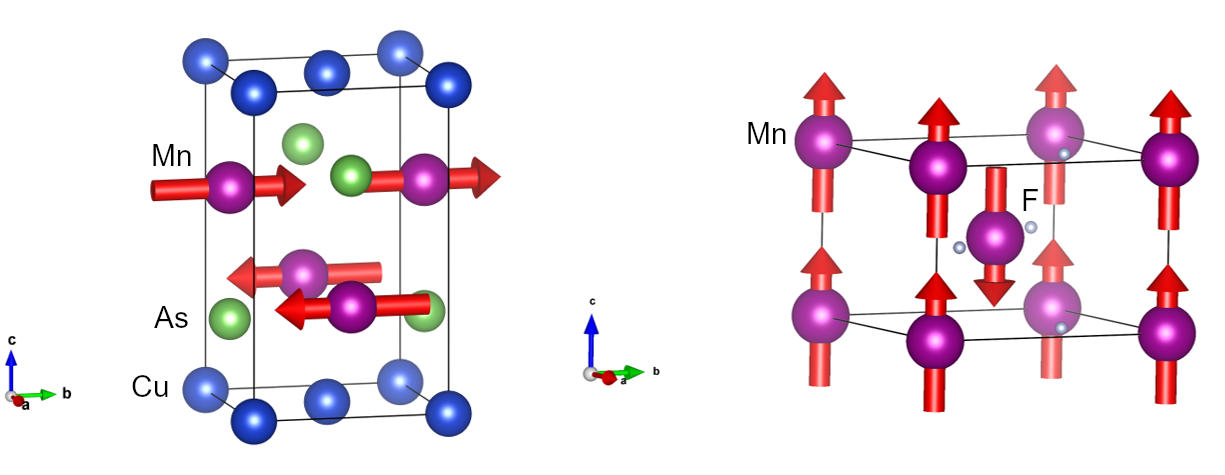
\includegraphics[width=\columnwidth]{figures/ch1/CuMnAs-MnF2.png} \\
\caption{\label{fig:tet-CuMnAs}
The magnetic structures of tetragonal CuMnAs and MnF$_2$ are shown in (a) and (b), respectively.
}
\end{figure}

\section{Exploration of Cu-Mn-As phase space}

% Why are CuMnAs compounds popular?
Compounds in Cu-Mn-As phase space have attracted a lot of attention in recent times mainly due to the exotic properties of tetragonal and orthorhombic CuMnAs. As mentioned earlier, tetragonal CuMnAs was the first antiferromagnet where electrical switching was supposedly demonstrated. Orthorhombic CuMnAs, shown in Fig. \ref{fig:ort-CuMnAs}, was the first magnetic compound to be proposed as a Dirac semimetal. It is a special compound where the inversion and time reversal symmetry of the magnetic structure is broken but their combined symmetry ($PT$ symmetry) is still preserved. Based on the orientation of the AFM order parameter, the compound changes from a conducting to an insulating phase. Hence, there are voltage based switching applications that have been proposed for this compound \cite{Kim2018}.

\begin{figure}
\centering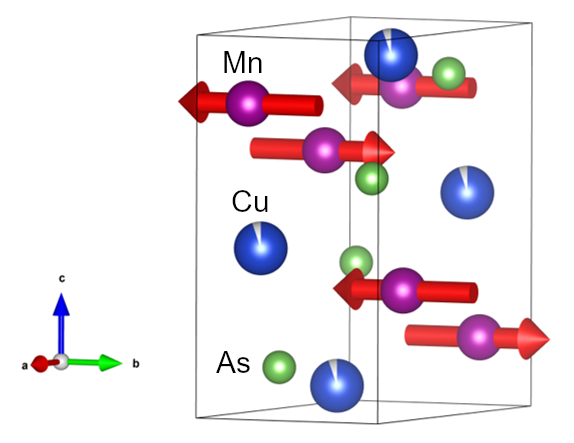
\includegraphics[width=0.5\columnwidth]{figures/ch1/ort-CuMnAs.png} \\
\caption{\label{fig:ort-CuMnAs}
Magnetic structure of orthorhombic CuMnAs
}
\end{figure}


\begin{figure}
\centering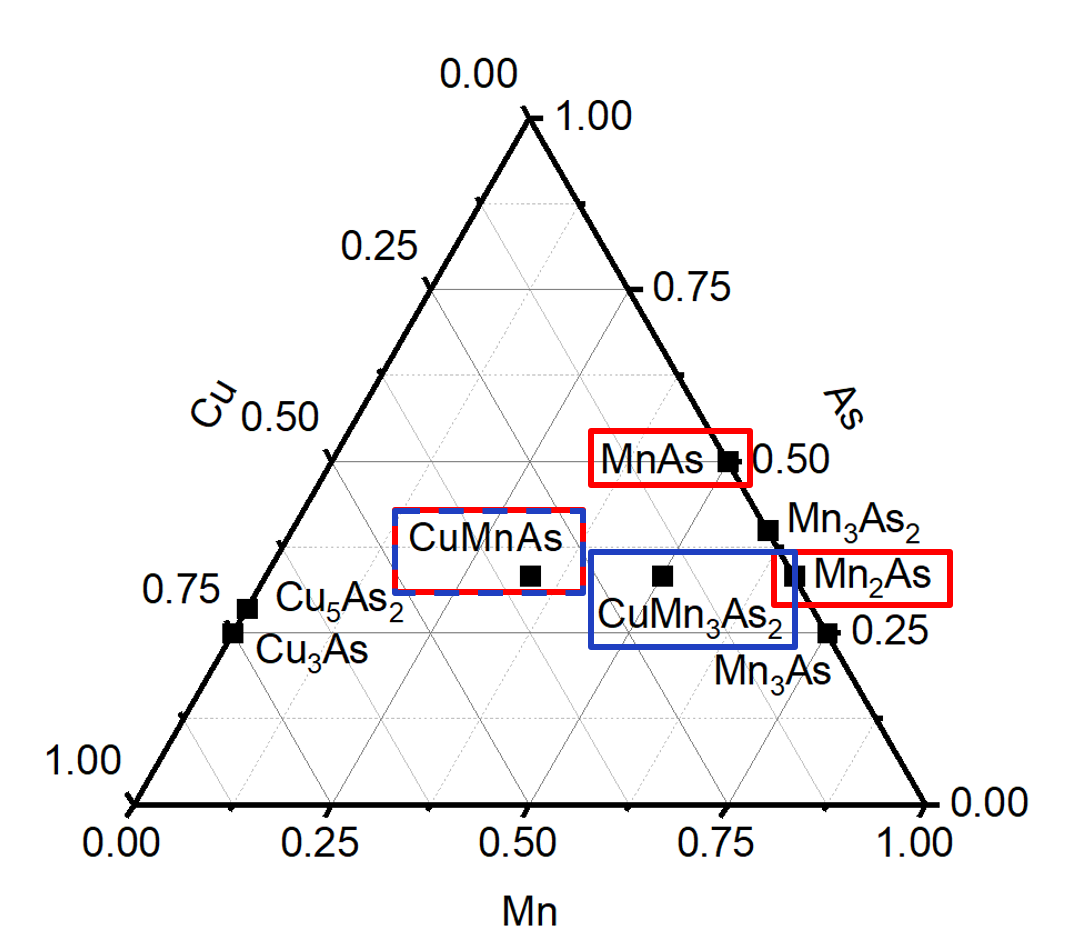
\includegraphics[width=0.8\columnwidth]{figures/ch1/Cu-Mn-As phase diagram.png} \\
\caption{\label{fig:Cu-Mn-As}
Cu-Mn-As ternary phase diagram highlighting some of the known ternary compounds in blue and known magnetic structures in red. Not all compounds in this system are shown here.
}
\end{figure}


% The dual problem
Despite the growing importance of the compounds in Cu-Mn-As system, the Cu-Mn-As ternary phase space has not been explored properly. There are four known ternary compounds including both the polymorphs of CuMnAs, orthorhombic CuMn$_3$As$_2$ and Cu$_2$Mn$_4$As$_3$ as shown in Fig. \ref{fig:Cu-Mn-As} \cite{Nateprov2011,MacA2012,Wadley2013,Uhlirova2015}. Bulk orthorhombic CuMnAs can be grown using traditional solid state synthesis routes by Cu, Mn and As powders in stoichiometric ratio and heating the powders to 1000$^\circ$C. In order to synthesize pure bulk tetragonal CuMnAs, we have to go off-stoichiometry and either substitute Mn with Cu or As \cite{Uhlirova2015}. Hence, it is important to explore different regions in the Cu-Mn-As system and verify the stability of different ternary compounds. The magnetic structures in the Cu-Mn-As system have also not been identified for most of the compounds. Apart from the four Cu-Mn-As ternary compounds, there are more than ten Mn-As binary compounds present in this system. The magnetic structures are known only for the two previously mentioned CuMnAs compounds, Mn$_2$As and MnAs as shown in Fig. \ref{fig:Cu-Mn-As} \cite{MacA2012,Wadley2013,Hills2015,Wadley2015,Austin1962,Bacon1955}. Since most, if not all, the binary Mn-As compounds are metallic, there is a need to magnetically characterize the compounds and identify their magnetic structures.

\section{Exchange interactions in Cu$_2$Sb type structures}

% Exchange interactions in Cu$_2$Sb materials.
If we want to understand the electrical switching behavior in metallic antiferromagnets, we should be able to quantify the fundamental energies such as magnetocrystalline anisotropy and exchange interactions in materials like CuMnAs. CuMnAs has a Cu$_2$Sb structure type. Other materials with this structure includes Mn$_2$As, Cr$_2$As, Fe$_2$As, CrMnAs, MnFeAs etc. \cite{Lutz-Kappelman2018,Zhang2013,Zhang2015}. Although Mn$_2$As, Cr$_2$As and Fe$_2$As have the same structure, the magnetic ground state is different in all three compounds. The strength and sign of direct exchange interactions between two magnetic atoms is a result of the nature of orbital overlap between the two magnetic atoms \cite{Zhang2013}. Since these materials are metallic, there are two contributions to indirect exchange interactions. One contribution arises from superexchange interactions mediated by As atoms and the other contribution comes from RKKY (Ruderman–Kittel–Kasuya–Yosida) interactions \cite{Zhang2015}. It is important that we are able to determine what spin interactions are relevant and how does it affect the magnetic ordering in these materials. It is also crucial that we are able to verify the computational methods and the exchange coupling values obtained from these methods so that we can use these methods for other systems as well.

%##################chapter 2
\chapter{Theory of electrical switching in metallic antiferromagnets}

%Introduction
Electrical switching in any magnetic compound is a series of events involving current induced spin polarization (CISP) of charge carriers and different components of CISP exerting different torque on the magnetic moments of the atoms. The nature of CISP is set by the crystal symmetry. In previous studies of CuMnAs and Mn$_2$Au, it was stated that the compound should globally centrosymmetric but locally non-centrosymmetric and the two sublattices should be related to each other by a center of inversion \cite{Zelezny2014,Zelezny2017,Wadley2016}. Is this a necessary condition for observing a staggered spin polarization configuration and can it be applied to general cases? These are some of the questions we will answer in this chapter. Once we have determined the required symmetry criteria, we will filter out metallic antiferromagnetic candidates from large databases of materials such as MPDS (Materials Platform for Data Science) and ASM (ASM International), and analyze the effect of CISP on the torque experienced by the order parameter.

\section{Hidden spin polarization in centrosymmetric crystals}

% Explanation of R2-D2 effect
It has been known for quite some time that in materials (even non-magnetic) having large spin orbit coupling (SOC) and lacking a center of inversion, magnetic fields are induced. When materials possess structural inversion asymmetry such as in quantum wells and other heterostructures, this effect is called the Rashba effect and it results in a helical type spin texture. When this occurs in materials that lack bulk inversion symmetry, the effect is called the Dresselhaus effect and it results in a unique spin texture \cite{Zhang2014}. Zhang \emph{et al.} \cite{Zhang2014} argued that since SOC is a relativistic effect, instead of considering the symmetry of the entire unit cell, one should check for atomic site symmetry to understand SOC induced spin polarization. Based on this argument, there are four cases possible as shown in Table \ref{tab:RD_effect}.

R1 and D1 effects refer to conventional Rashba and Dresselhaus spin polarization respectively. In materials that are globally centrosymmetric, hidden spin polarization is possible. There is local spin polarization near non-centrosymmetric sites but when summed over the entire unit cell, the net spin polarization is zero. This effect is called the R2 or D2 effect corresponding to Rashba or Dresselhaus effect, respectively in centrosymmetric crystals. The total spin polarization of the unit cell is the vector sum of all the local spin polarizations in the unit cell. Non-centrosymmetric point groups can be further divided into polar and non-polar groups. Local Rashba effect requires the presence of polar point groups on atomic sites and the local Dresselhaus effect requires the presence of non-polar point groups at the atom sites. The presence of local spin polarization in centrosymmetric crystals opens the avenue for studying spin polarization in a larger group of compounds including metallic antiferromagnets.

\renewcommand{\arraystretch}{1.2}
\begin{table}
\caption{\label{tab:RD_effect} 
Different cases of spin polarization depending on the symmetry of atomic sites and the unit cell \cite{Zhang2014}.}
\centering
\begin{tabular}{>{\raggedright\arraybackslash}p{5cm}>{\raggedright\arraybackslash}p{3cm}>{\raggedright\arraybackslash}p{3cm}>{\raggedright\arraybackslash}p{3cm}}
\hline\hline
\textbf{} & \textbf{All non-polar point groups} & \textbf{At least one polar point groups} & \textbf{All centrosymmetric point groups}\\
\hline
\textbf{Non-Centrosymmetric space group} & D1 effect & R1/D1 effect & Not possible\\
\hline
\textbf{Centrosymmetric space group} & D2 effect & R2/D2 effect & No spin polarization\\
\hline\hline
\end{tabular}
~\\
\end{table}

\section{Finding metallic antiferromagnetic candidates with R2-D2 effect}

% Replace this figure maybe
\begin{figure}
\centering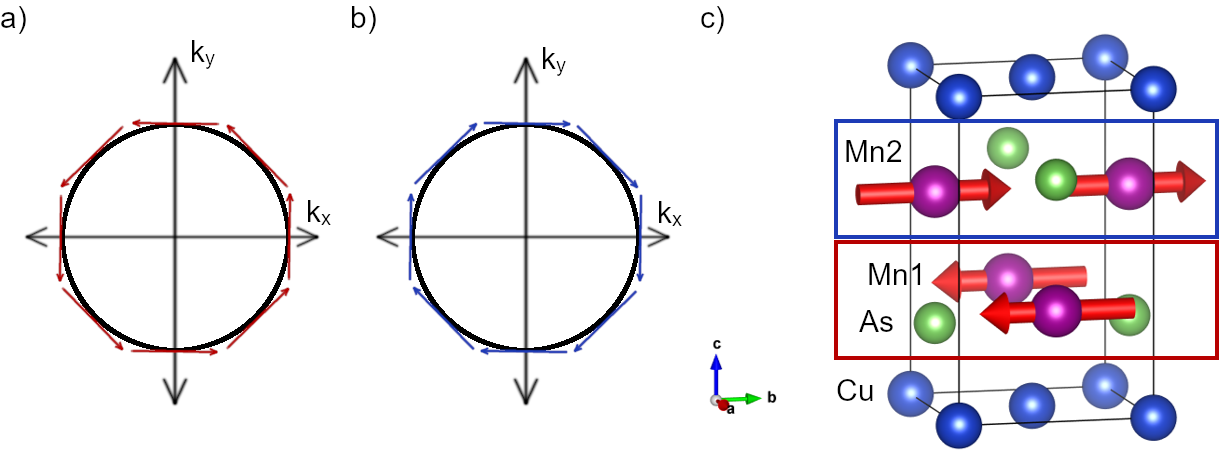
\includegraphics[width=\columnwidth]{figures/ch2/wadley_1.png} \\
\caption{\label{fig:wadley_1}
The schematic of the Fermi surface of the local sectors near Mn1 and Mn2 atoms are shown in (a) and (b), respectively. The magnetic structure of tetragonal CuMnAs is shown in (c) which also includes the highlighted local sectors.
}
\end{figure}

% Explain use of Zunger paper in CuMnAs

In spin orbit torque based switching of metallic antiferromagnets, the same arguments apply as before except that we only care about the point group symmetry at the magnetic atom sites. For example, the magnetic structure of CuMnAs is shown in Fig. \ref{fig:wadley_1}(c). Cu and As atoms have no moments and sit on D$_{2d}$ and C$_{4v}$ sites, respectively. Since only the Mn atoms have moments, we must take the site symmetry of Mn atoms into consideration. Mn atom sites have C$_{4v}$ point group symmetry which is polar. As seen in Fig. \ref{fig:wadley_1}(a,b), the schematic of the Fermi surface corresponding to the Mn layer has a Rashba-like spin texture. When the current is applied, through inverse spin galvanic effect, there is a spin polarization of the conduction electrons near Mn sites. The spin polarization is staggered across the two Mn sublattices and through exchange coupling, a torque is experienced by the Mn moments. From the example of CuMnAs above, we can search for compounds from databases that are antiferromagnets or are likely to be antiferromagnets where the magnetic atoms sit on a polar point group. Such a search can be made for compounds which are not complicated by the presence of many magnetic sites with different point groups. The general case applicable for all magnetic compounds will be considered in the following sections. Following is the general procedure for extracting potential metallic antiferromagnet candidates from databases -

% Procedure list
\begin{enumerate}
\item Search for known metallic antiferromagnets from database having tetragonal, trigonal or hexagonal crystal system.
\item Remove duplicate and non-centrosymmetric compounds.
\item Identify the Néel temperature and magnetic ordering.
\item Filter out compounds having Néel temperature $>$ 300 K.
\item Identify the nature of atomic site symmetry and select compounds.
\item Study available literature to see if any compounds can be synthesized as single crystals.
\end{enumerate}

This procedure assumes that we are starting with a collection of known or possible metallic antiferromagnets. This is true in case of compounds downloaded from MPDS. In case of ASM database, the compounds are metallic but their magnetism is not known beforehand. We will have to make some assumptions based on the chemical nature and stoichiometry of the ions present in the compound in order to select possible antiferromagnets. Tetragonal, trigonal or hexagonal crystal systems are preferred since they allow for the presence of multiple degenerate axes for N\'eel vector orientation. It is still important to check if the magnetic structure for the compound is known or not and if the N\'eel vector points along the degerate axes. Carrying out the above mentioned steps for compounds in MPDS and ASM database gives us a list of compounds  in Table \ref{tab:metallic_afm_candidates} that have been grouped together based on their structure types.

\renewcommand{\arraystretch}{1.2}
\begin{table}
\caption{\label{tab:metallic_afm_candidates} 
List of metallic antiferromagnetic candidates filtered out from MPDS and ASM database and their metal atom site symmetries}
\centering
\begin{tabular}{>{\raggedright\arraybackslash}p{3cm}>{\raggedright\arraybackslash}p{4cm}>{\centering}p{3cm}>{\raggedright\arraybackslash}p{4cm}}
\hline\hline
\textbf{Structure type} & \textbf{List of compounds} & \textbf{Point group} & \textbf{Magnetism}\\
\hline
MoSi$_2$ & Mn$_2$Au, Cr$_2$Al, Ni$_2$Ta & C$_{4v}$ & Mn$_2$Au is a known candidate\\
\hline
HfFe$_6$Ge$_6$ & ScFe$_6$Ge$_6$ & C$_{2v}$ & AFM with N\'eel vector along $c$\\
\hline
Mg$_3$Cd & Mn$_3$Ga, Mn$_3$Ge, Mn$_3$Sn, Fe$_3$Ga, Co$_3$Mo, Co$_3$W, Ni$_3$In, Ni$_3$Sn, Ni$_3$Zr & C$_{2v}$ & Non-collinear AFM\\
\hline
IrIn$_3$ & CoGa$_3$, CoIn$_3$, FeGa$_3$ & C$_{2v}$ & FeGa$_3$ and CoGa$_3$ are diamagnets\\
\hline
MoNi$_4$ & MoNi$_4$, WNi$_4$ & C$_{1v}$ & Unknown\\
\hline
Ni$_2$Al$_3$ & Ni$_2$Al$_3$, Ni$_2$Ga$_3$, Ni$_2$In$_3$ & C$_{3v}$ & Unknown\\
\hline\hline
\end{tabular}
~\\
\end{table}

%Discuss the list of compounds obtained

The first group of compounds consist of materials in MoSi$_2$ structure type. Mn$_2$Au is a well-known compound that has been extensively studied for electrical switching applications \cite{Meinert2018,Bodnar2019}. Cr$_2$Al powders can be prepared using traditional solid state synthesis routes by heating to above 850$^\circ$C \cite{Susner2015}. Early neutron diffraction experiments suggest Cr moments align at 65$^\circ$ to the $ab$ plane \cite{Atoji1965}. However, a later article indicates that the determined magnetic structure may not be correct \cite{Kallel1967}. Regardless of whether the moments align in the $ab$ plane or not, Cr$_2$Al is an interesting candidate to study electrical switching behavior. ScFe$_6$Ge$_6$ is AFM at room temperature \cite{Venturini1992}. However, the Fe moments align along $c$ and does not satify our criteria \cite{Mazet2000}. Compounds in the Mg$_3$Cd structure type contain Kagome lattice of magnetic atoms. Mn$_3$Sn and Mn$_3$Ge are known to have a non-collinear spin arrangement. They have become popular recently for showing large anomalous hall and spin hall effect behavior \cite{Nakatsuji2015,Kubler2014,Kimata2019}. Electrical switching was also demonstrated in Mn$_3$Sn recently. In the fourth group of compounds, both FeGa$_3$ and CoGa$_3$ are known to show diamagnetic properties and hence they can be discarded \cite{Haussermann2002,Viklund2002,Zhang2017}. The magnetism is unknown in the final two groups of compounds in MoNi$_4$ and Ni$_2$Al$_3$ structure types and most of these compounds can be synthesized by the arc melting process \cite{Harker1944,Taylor1972}.

\section{Components of torque from non-equilibrium CISP}

% Zelezny 2017 paper

The previous section dealt with relatively simple magnetic compounds that had only one magnetic atom site and we were concerned with the point group of the site to determine whether the inverse spin galvanic effect would be observed or not. In the simplest sense, antidamping-like STT is induced by spin hall effect (SHE) and fieldlike SOT is generated from inverse spin galvanic effect. However, incomplete absorption of the spin current from SHE by the FM layer may produce a fieldlike torque, and spin relaxation and damping may induce an antidamping like component to the SOT \cite{Zelezny2017}. Using Kubo linear formalism, we can write CISP $\delta S_a = \chi_a E$ where E is the applied electric field and $\chi_a$ is the linear response tensor for the sublattice a. $\chi_a$ can be further divided into three components:

\begin{equation}
\chi_a = \chi_a^I + \chi_a^{II(a)} + \chi_a^{II(b)}
\end{equation}

where $\chi_a^I$ is the intraband term, and $\chi_a^{II(a)}$ and $\chi_a^{II(b)}$ are the interband terms. $\chi_a$ can also be broken down into even and odd terms:

\begin{equation}
\chi_a = \chi_a^{even} + \chi_a^{odd}
\end{equation}

where $\chi_a^{even} = (\chi_a([M])+\chi_a([-M]))/2$ and $\chi_a^{odd} = (\chi_a([M])-\chi_a([-M]))/2$. From the symmetry of the operators and the matrix element, it follows that -

\begin{equation}
\chi_a^{even} = \chi_a^{I} + \chi_a^{II(b)}
\end{equation}
\begin{equation}
\chi_a^{odd} = \chi_a^{II(a)}
\end{equation}

We assume that the system only has a weak disorder and hence, we can neglect $\chi_a^{II(b)}$. $\chi_a$ also depends on the direction of the magnetic moments where \^n is the direction of the N\'eel vector.

\begin{equation}
\chi_{a,i,j}(\hat{n}) = \chi_{a,i,j}^{(0)} + \chi_{a,i,j,k}^{(1)}\hat{n}_k + \chi_{a,i,j,k,l}^{(2)}\hat{n}_k\hat{n}_l + ...
\end{equation}

where the sum of the first term and every alternate term after that corresponds to $\chi_a^{even}$ and the sum of the remaining terms correspond to $\chi_a^{odd}$. $\chi_a^{(0)}$ is usually dominant, independent of magnetization and contributes to field-like torque. $\chi_a^{(1)}$ contributes to anti-damping like torque and $\chi_a^{(2)}$ can be neglected if $\chi_a^{(0)}$ is not 0 \cite{Zelezny2017}. The zeroth order term which contributes to a fieldlike torque consists of three components in the form of generalized Rashba and generalized Dresselhaus terms and a term that is proportional to the electric field as shown by the following equations:

\begin{equation}
\text{Generalized Rashba } \chi_a^{gR} = \begin{bmatrix} \chi_{11} & -\chi_{21} & 0 \\ \chi_{21} & \chi_{11} & 0 \\ 0 & 0 & 0 \end{bmatrix}
\end{equation}

\begin{equation}
\text{Generalized Dresselhaus } \chi_a^{gD} = \begin{bmatrix} \chi_{11} & \chi_{21} & 0 \\ \chi_{21} & -\chi_{11} & 0 \\ 0 & 0 & 0 \end{bmatrix}
\end{equation}

\begin{equation}
\text{Proportional to Electric field } \chi_a^{E} = \begin{bmatrix} \chi_{11} & 0 & 0 \\ 0 & \chi_{11} & 0 \\ 0 & 0 & \chi_{11} \end{bmatrix}
\end{equation}



Similarly, the first order term can also be broken into three different components \cite{Zelezny2017}. The summary of the linear response tensor components is also provided in the Table \ref{tab:chi_summary}

\renewcommand{\arraystretch}{1.3}
\begin{table}
\caption{\label{tab:chi_summary} 
Summary of the linear response tensor components for the CISP observable and electric field}
\centering
\begin{tabular}{>{\raggedright\arraybackslash}p{3.5cm}>{\raggedright\arraybackslash}p{3.5cm}>{\raggedright\arraybackslash}p{3.5cm}>{\raggedright\arraybackslash}p{3.5cm}}
\hline\hline
 & \boldmath{$\chi_a^I$} & \boldmath{$\chi_a^{II(a)}$} & \boldmath{$\chi_a^{II(b)}$}\\
\hline
\textbf{Component} &  Intraband & Interband (imaginary) & Interband (real)\\
\hline
\textbf{Disorder $\Gamma \rightarrow 0$} &  Diverges & Constant & Zero\\
\hline
\textbf{Cause} & Non-equilibrium Fermi-Dirac distribution & Intrinsic change in carrier wave function & Change in carrier wave function due to disorder/defects\\
\hline
\textbf{Alternate name} & $\chi_a^{even}$ or $\chi_a^{(0)}$ & $\chi_a^{odd}$ or $\chi_a^{(1)}$ & \\
\hline
\textbf{Dependence on magnetization} & Independent & Dependent & \\
\hline
\textbf{Torque} & Field-like & Anti-damping-like & \\
\hline\hline
\end{tabular}
~\\
\end{table}

\section{Spin polarization in CuMnAs, Mn$_2$Au and Fe$_2$As}

% Provide examples from code.

Zelezny \emph{et al.} \cite{Zelezny2017} provides a python code $symmetr$ for analyzing the linear response tensor for a number of observables such as current, spin, torque, position, spin current etc. and electric field. Using this code, we can test the reponse tensor of known compounds such as CuMnAs and Mn$_2$Au and also check for unknown compounds such as Fe$_2$As. Table \ref{tab:CISP_CuMnAs} shows the linear response tensor in case of CuMnAs or Mn$_2$Au. Both compounds have same spin polarization since they are both globally centrosymmetric and Mn atoms sit on C$_{4v}$ point group sites. Let us first understand $\chi^{even}$ for all the different cases presented here. Magnetism can be turned off to avoid including magnetization-based effects to the reponse tensor. Regardless of whether we toggle magnetism in Mn atoms or not, $\chi^{even}$ is 0 for the whole unit cell since it is centrosymmetric. When Mn magnetic moment is set to 0, $\chi^{even}$ for each sublattice corresponds to the response in conventional Rashba spin texture. Regardless of magnetism, the spin polarization in one site is opposite to that of another site as seen in the projected cases. When magnetism is turned on, $|\chi_{10}| = |\chi_{01}|$ is not valid anymore since we also have to consider higher terms in $\chi^{even}$. In case of $\chi^{odd}$, it is 0 when magnetization is turned off as also shown in Table \ref{tab:chi_summary}. When magnetic moments are allowed, there is spin polarization along $c$ direction.

\begin{table}
\caption{\label{tab:CISP_CuMnAs} 
Linear response tensor in CuMnAs and Mn$_2$Au assuming Mn moment to be 1 $\mu_B$.}
\centering
\begin{tabular}{>{\raggedright\arraybackslash}p{7cm}>{\centering\arraybackslash}p{3.5cm}>{\centering\arraybackslash}p{3.5cm}}
\hline\hline
\addlinespace[1.5ex]
 & \boldmath{$\chi^{even}$} & \boldmath{$\chi^{odd}$} \\
\addlinespace[1.5ex]
\hline
\addlinespace[1.5ex]
\textbf{Magnetic Mn. For the entire unit cell} & $\begin{bmatrix} 0 & 0 & 0\\ 0 & 0 & 0\\  0 & 0 & 0\\ \end{bmatrix}$ & $\begin{bmatrix} 0 & 0 & \chi_{02}\\ 0 & 0 & 0\\  \chi_{20} & 0 & 0 \end{bmatrix}$ \\
\addlinespace[1.5ex]
\hline
\addlinespace[1.5ex]
\textbf{Magnetic Mn. For each Mn sublattice} &  $\begin{bmatrix} 0 & \chi_{01} & 0\\ \chi_{10} & 0 & 0\\  0 & 0 & 0\\ \end{bmatrix}$ & $\begin{bmatrix} 0 & 0 & \chi_{02}\\ 0 & 0 & 0\\  \chi_{20} & 0 & 0\end{bmatrix}$\\
\addlinespace[1.5ex]
\hline
\addlinespace[1.5ex]
\textbf{Magnetic Mn. For one Mn sublattice projected onto another} & $\begin{bmatrix} 0 & -\chi_{01} & 0\\  -\chi_{10} & 0 & 0\\  0 & 0 & 0\\ \end{bmatrix}$ & $\begin{bmatrix} 0 & 0 & \chi_{02}\\ 0 & 0 & 0\\  \chi_{20} & 0 & 0\end{bmatrix}$\\
\addlinespace[1.5ex]
\hline
\addlinespace[1.5ex]
\textbf{Non-magnetic Mn. For the entire unit cell} & $\begin{bmatrix} 0 & 0 & 0\\ 0 & 0 & 0\\  0 & 0 & 0\\ \end{bmatrix}$ & $\begin{bmatrix} 0 & 0 & 0\\ 0 & 0 & 0\\ 0 & 0 & 0\\ \end{bmatrix}$\\
\addlinespace[1.5ex]
\hline
\addlinespace[1.5ex]
\textbf{Non-magnetic Mn. For each Mn sublattice} & $\begin{bmatrix} 0 & -\chi_{10} & 0\\ \chi_{10} & 0 & 0\\  0 & 0 & 0\\ \end{bmatrix}$ & $\begin{bmatrix} 0 & 0 & 0\\ 0 & 0 & 0\\ 0 & 0 & 0\\ \end{bmatrix}$\\
\addlinespace[1.5ex]
\hline
\addlinespace[1.5ex]
\textbf{Non-magnetic Mn. For one Mn sublattice projected onto another} & $\begin{bmatrix} 0 & \chi_{10} & 0\\ -\chi_{10} & 0 & 0\\  0 & 0 & 0\\ \end{bmatrix}$ & $\begin{bmatrix} 0 & 0 & 0\\ 0 & 0 & 0\\ 0 & 0 & 0\\ \end{bmatrix}$\\
\addlinespace[1.5ex]
\hline\hline
\end{tabular}
~\\
\end{table}

Table \ref{tab:CISP_Fe2As} shows linear response tensor components in Fe$_2$As. Fe$_2$As is complicated by the presence of two different Fe sites. Fe1, Fe2, Fe5 and Fe6 atoms shown in Fig. \ref{fig:Fe2As} sit on D$_{2d}$ site whereas Fe3, Fe4, Fe7 and Fe8 atoms sit on C$_{4v}$ sites. The table only shows cases where Fe moments have not been considered. However, the results with finite Fe moments in case of $\chi^{even}$ can be easily inferred from this table by removing the equality between the magnitudes of $\chi_{ij}$ and $\chi_{ji}$. As expected, $\chi^{odd}$ is a zero matrix when magnetism is turned off. $\chi^{even}$ is 0 when the entire unit cell is considered which is expected since the unit cell is centrosymmetric like in the previous case. The sublattices Fe3 and Fe4 sitting on polar point groups show conventional Rashba spin polarization behavior. When $\chi^{even}$ at Fe3 is projected onto Fe4, we can see that the response is exactly opposite to Fe4. In case of sublattices Fe1 and Fe2 sitting on non-polar point groups, $\chi^{even}$ corresponds to generalized Dresselhaus polarization when $\chi_{00}$ and $\chi_{11}$ have been set to 0. As expected, the spin polarization would be opposite on the two sublattices. The nature of $\chi^{odd}$ when magnetism is included has not been discussed here.



\begin{table}
\caption{\label{tab:CISP_Fe2As} 
Linear response tensor in Fe$_2$As when Fe moments have been set to 0 $\mu_B$.}
\centering
\begin{tabular}{>{\raggedright\arraybackslash}p{7cm}>{\centering\arraybackslash}p{3.5cm}>{\centering\arraybackslash}p{3.5cm}}
\hline\hline
\addlinespace[1.5ex]
 & \boldmath{$\chi^{even}$} & \boldmath{$\chi^{odd}$} \\
\addlinespace[1.5ex]
\hline
\addlinespace[1.5ex]
\textbf{For the entire unit cell} & $\begin{bmatrix} 0 & 0 & 0\\ 0 & 0 & 0\\  0 & 0 & 0\\ \end{bmatrix}$ & $\begin{bmatrix} 0 & 0 & 0 \\ 0 & 0 & 0\\  0 & 0 & 0 \end{bmatrix}$ \\
\addlinespace[1.5ex]
\hline
\addlinespace[1.5ex]
\textbf{For Fe1 and Fe2} &  $\begin{bmatrix} 0 & \chi_{10} & 0\\ \chi_{10} & 0 & 0\\  0 & 0 & 0\\ \end{bmatrix}$ & $\begin{bmatrix} 0 & 0 & 0 \\ 0 & 0 & 0\\  0 & 0 & 0 \end{bmatrix}$\\
\addlinespace[1.5ex]
\hline
\addlinespace[1.5ex]
\textbf{For Fe3 and Fe4} & $\begin{bmatrix} 0 & -\chi_{10} & 0\\  \chi_{10} & 0 & 0\\  0 & 0 & 0\\ \end{bmatrix}$ & $\begin{bmatrix} 0 & 0 & 0 \\ 0 & 0 & 0\\  0 & 0 & 0 \end{bmatrix}$\\
\addlinespace[1.5ex]
\hline
\addlinespace[1.5ex]
\textbf{For Fe1 projected onto Fe2} & $\begin{bmatrix} 0 & -\chi_{10} & 0\\ -\chi_{10} & 0 & 0 \\  0 & 0 & 0\\ \end{bmatrix}$ & $\begin{bmatrix} 0 & 0 & 0\\ 0 & 0 & 0\\ 0 & 0 & 0\\ \end{bmatrix}$\\
\addlinespace[1.5ex]
\hline
\addlinespace[1.5ex]
\textbf{For Fe3 projected onto Fe4} & $\begin{bmatrix} 0 & \chi_{10} & 0\\ -\chi_{10} & 0 & 0\\  0 & 0 & 0\\ \end{bmatrix}$ & $\begin{bmatrix} 0 & 0 & 0\\ 0 & 0 & 0\\ 0 & 0 & 0\\ \end{bmatrix}$\\
\addlinespace[1.5ex]
\hline
\addlinespace[1.5ex]
\textbf{For Fe1 projected onto Fe3} & No relation & No relation \\
\addlinespace[1.5ex]
\hline\hline
\end{tabular}
~\\
\end{table}

\begin{figure}
\centering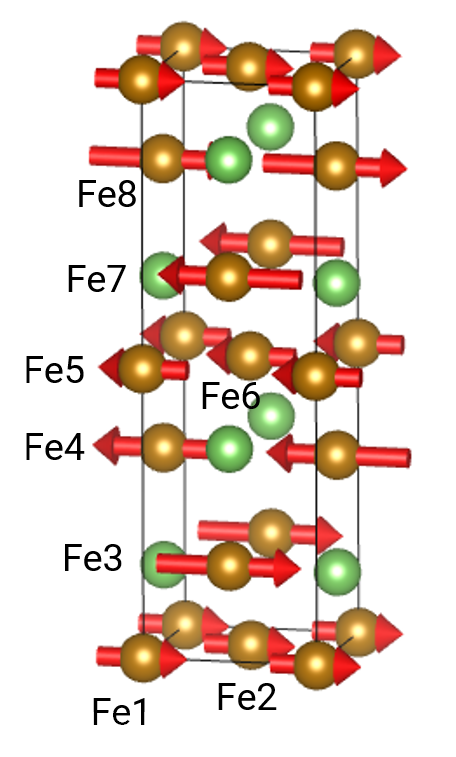
\includegraphics[width=0.3\columnwidth]{figures/ch2/Fe2As.png} \\
\caption{\label{fig:Fe2As}
Magnetic structure of Fe$_2$As along with the Fe site numbers corresponding to Table \ref{tab:CISP_Fe2As}.
}
\end{figure}

\section{Conclusions}

There can be local spin polarization present even in centrosymmetric crystals provided the unit cell contains non-centrosymmetric point groups. In CISP based switching, it is important that the magnetic ions sit on non-centrosymmetric sites. The presence of polar point group is required for Rashba spin polarization and non-polar point group for Dresselhaus spin polarization. We need to consider both antidamping-like torque and fieldlike torque when considering spin polarization. In broken inversion symmetry 2D AFM, it is the antidamping-like torque that can provide a mechanism for switching since the fieldlike torque component of CISP is uniform. In Fe$_2$As, CISP from ISGE in Fe3 and Fe4 sublattices is similar to Mn in CuMnAs. However, there is no relation between the even component of CISP in Fe1 or Fe2 and Fe3 or Fe4 sublattices. This allows for two possibilities when the current is along $[100]$. If the torque acts in the same direction for both sets of Fe atoms, then it would provide a possible pathway for switching. However, if the fieldlike torque act in the opposite direction for both sets of Fe moments, then a large current threshold may be required before the moments can be possibly switched.

\section{Acknowledgements}

% Acknowledge Scott and Carmen

I would like to acknowledge two REU students, Scott Berens and Carmen Paquette, for compiling the list of metallic antiferromagnets from MPDS and ASM databases respectively. It saved me a lot of time and I was able to analyze the symmetry requirements on a much smaller list of compounds.





%##################chapter 3
\chapter{Materials synthesis and characterization}

\section{Bulk materials synthesis}

%As : Arsenic Polycrystalline lump, 2-8mm (0.08-0.3 in.), Puratronic, 99.9999% (Metals basis), Alfa Aesar
%Mn : 99.98% metals basis
%Cu : Copper powder, spherical, -100+325 mesh, 99.9% (metals basis), Alfa Aesar
%Fe old : Iron powder, -200 mesh, 99+% (metals basis), Alfa aesar
%Fe new : Iron powder, spherical, >99.99% (metal basis), 99.5%, Alfa Aesar

% Traditional solid state synthesis technique and provide ref to figures

% Note: You may include pycnometry data if time permits

Bulk polycrystalline and single crystals of all the samples are prepared by traditional solid state synthesis routes. The process of synthesizing these samples is shown in Fig. \ref{fig:synthesis_procedure}. The constituent elements of the compounds are mixed in certain ratio using a mortar and pestle in an Argon atmosphere glovebox shown in Fig. \ref{fig:synthesis_procedure}(a). Quartz tubes, that have been sealed from one side, are filled with the mixed elemental powders and vacuum sealed using a flame torch as shown in Fig. \ref{fig:synthesis_procedure}(b). The sealed quartz tubes in Fig. \ref{fig:synthesis_procedure}(c) are placed inside a box furnce and heated to a high temperature to allow the powders to fuse together as shown in Fig. \ref{fig:synthesis_procedure}(d). Upon cooling, the desired crystal is removed from the quartz tube and characterized.

\begin{figure}
\centering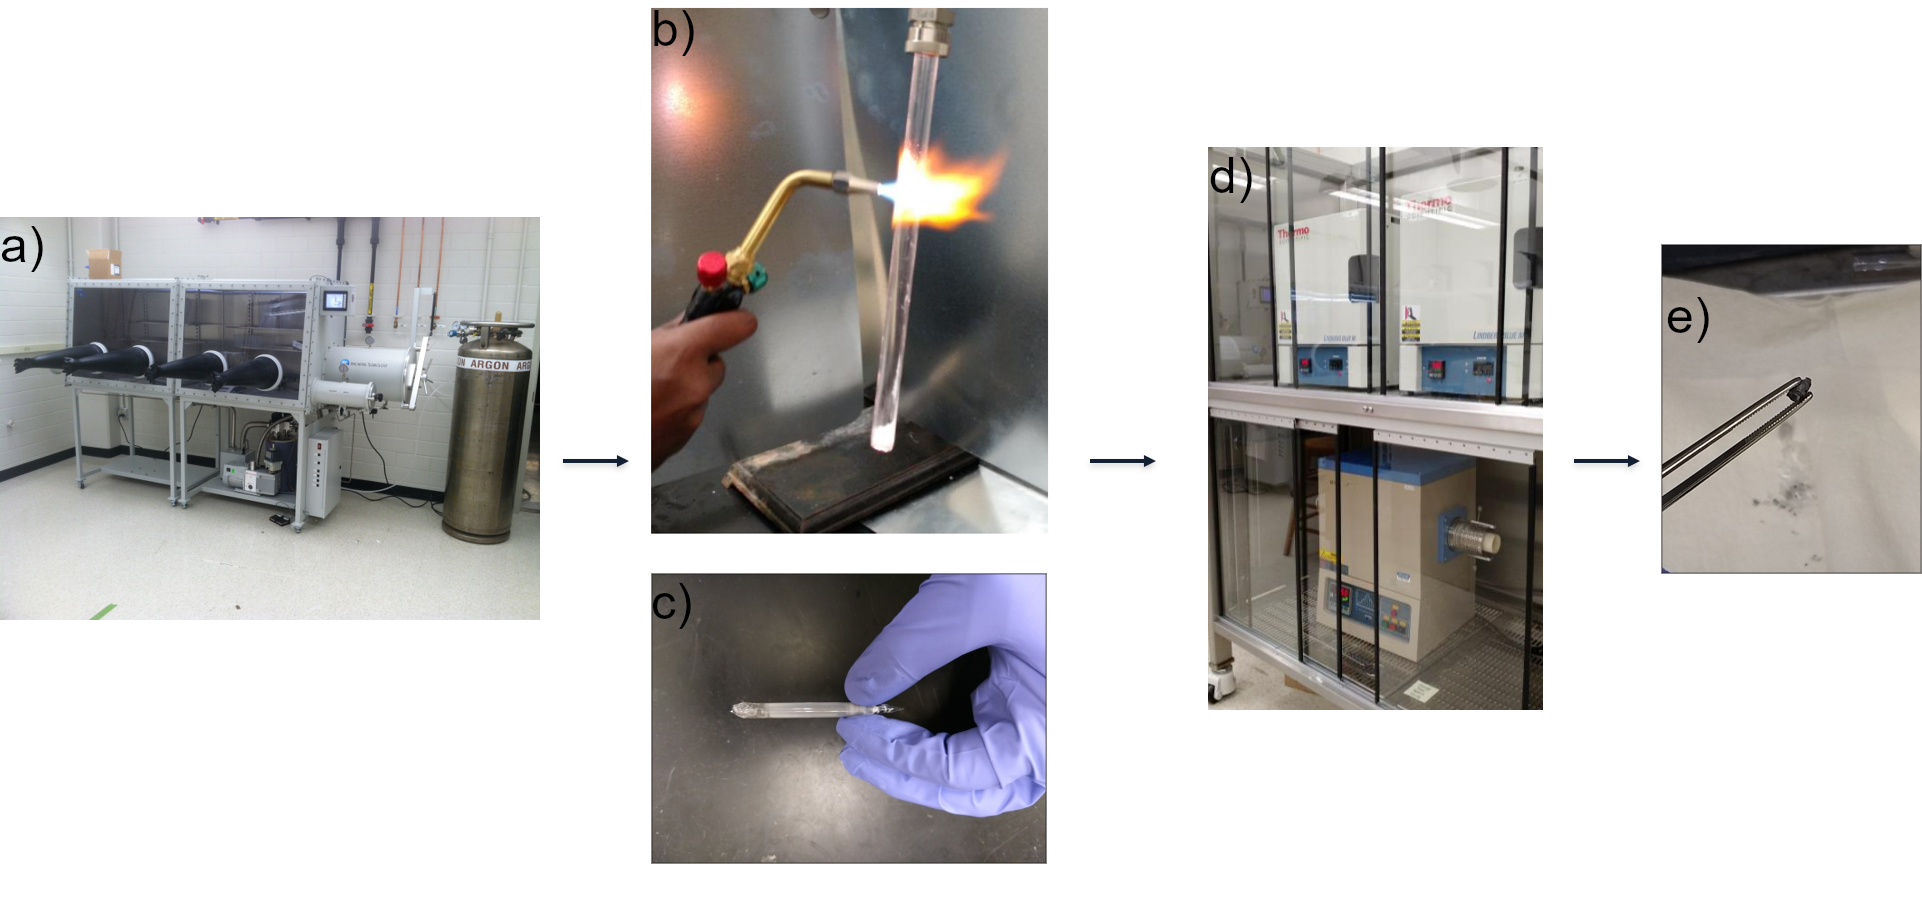
\includegraphics[width=\columnwidth]{figures/ch3/synthesis_procedure.png} \\
\caption{\label{fig:synthesis_procedure}
The process of making bulk materials using traditional solid state synthesis technique is shown here. The powders mixed inside the glovebox in (a) are transferred to a quartz tube and vacuum sealed in (b). The vacuum sealed ampoule in (c) is placed inside the box furnace in (d) and subjected to a heating profile. (e) shows the final ingot obtained in case of CuMnAs sample.
}
\end{figure}



\subsection{Sensitivity of Fe:As stoichiometry in the synthesis of Fe$_2$As}

% Fe2As and variation with stoichiometry
Fe$_2$As crystals are prepared by mixing Fe and As powders inside the glovebox and heating it up to 600$^\circ$C at 1$^\circ$C/min, holding it for 6 h and then heating it above the melting point to 975$^\circ$C at 1$^\circ$C/min. The sample is held at 975$^\circ$C for 1 h before cooling it down to 900$^\circ$C at 1$^\circ$C/min and held for 1 h. Finally, the sample is allowed to furnace-cool down to the room temperature. The source of the Fe powders seems to have significant effect on the optimum Fe:As starting stoichiometry. As powders were obtained by grinding As chunks (Alfa Aesar, 2-8mm, 99.9999\% (metals basis)) using a mortar and pestle. Fig. \ref{Fe2As_ratio_1} shows the impurity percentage as a function of Fe:As stoichiometry for Fe powders (Alfa Aesar, -200 mesh, 99+\% (metals basis)) with 0.74 $\mu$m in size. Phase pure Fe$_2$As is obtained for Fe:As ratio of 1.95:1. Increasing the Fe content results in Fe impurity and decreasing Fe content results in FeAs impurity.

\begin{figure}
\centering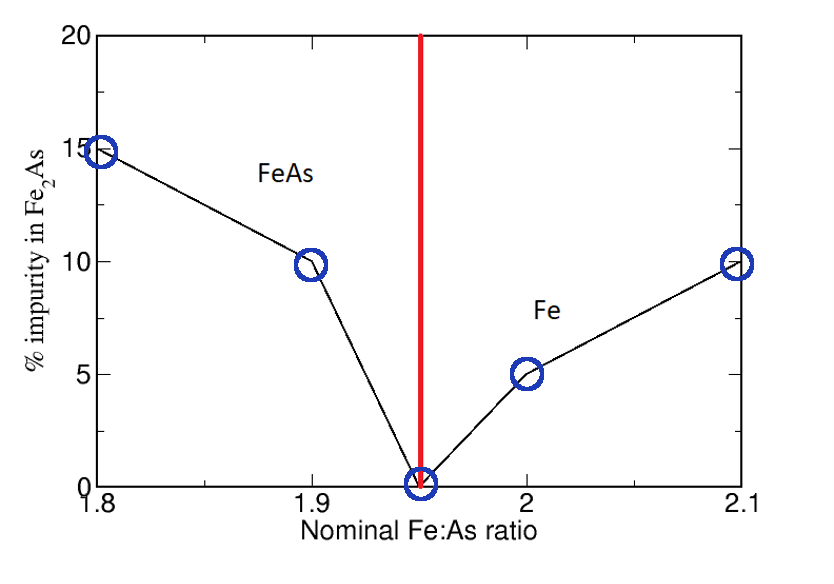
\includegraphics[width=0.5\columnwidth]{figures/ch3/Fe2As_ratio_1.png} \\
\caption{\label{fig:Fe2As_ratio_1}
Impurity percentage as a function of Fe:As starting stoichiometry ratio with 200 mesh size Fe powders for making Fe$_2$As samples.
}
\end{figure}

While using the 200 mesh size Fe powders yielded pure Fe$_2$As, the residual resistivity ratio from the transport measurements indicated Fe$_2$As to be a bad metal. In an attempt to reduce the presence of trace impurities, more pure Fe powders were sourced. Fe powders (Alfa Aesar, 10 $\mu$m, spherical, $>$99.99\% (metals basis)) with 10 $\mu$m in size were used for preparing batches of 1 g of Fe$_2$As crystals. In order to reduce processing errors, before vacuum sealing the quartz tube, a magnet was moved from top to bottom of the outer walls of the tube in a rocking fashion to remove any Fe powders sticking to the inner walls of the tube. Finally, the synthesized Fe$_2$As crystals were crushed into powders and sent to the 11-BM beamline at the Advanced Photon Source in Argonne National Laboratory for synchrotron x-ray diffraction measurements. The results of the 8 samples with different Fe:As ratio is shown in Fig. \ref{fig:Fe2As_ratio_2}(a). The results from this data suggest that Fe:As ratio of 2:1 which is also the stoichiometric ratio, is optimum to produce phase pure samples as shown in Fig. \ref{fig:Fe2As_ratio_2}(b). Similar to earlier results, increasing the Fe:As ratio above 2 precipitates out Fe impurity and decreasing the Fe:As ratio results in FeAs impurity. The region colored in purple in Fig. \ref{fig:Fe2As_ratio_2}(b) contained the opposite of the expected impurity. The purple region on the excess Fe side contained FeAs impurity and on the lower Fe side contained Fe impurity. I attribute this inconsistency to random errors.

\begin{figure}
\centering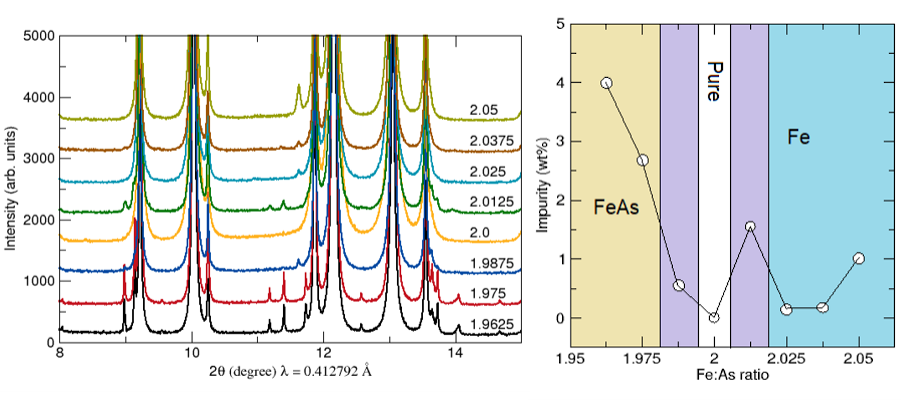
\includegraphics[width=\columnwidth]{figures/ch3/Fe2As_stoichiometry.png} \\
\caption{\label{fig:Fe2As_ratio_2}
Synchrotron x-ray diffraction data of Fe$_2$As for different ratios of Fe:As from 10 $\mu$m Fe powders is shown in (a) and the corresponding impurity percentage is shown in (b).
}
\end{figure}

\subsection{Synthesis of compounds in the Cu-Mn-As system}

%Synthesis of CuMnAs compounds

Compounds in the Cu-Mn-As system powders are synthesized by mixing Cu powders (Alfa Aesar, -100+325 mesh, spherical, 99.9\% (metals basis)), Mn powders ground from Mn chips (99.98\% (metals basis)) and As powders ground from chunks (Alfa Aesar, 2-8mm, 99.9999\% (metals basis)) inside the Ar atmosphere and following the same heating procedure as in the case of Fe$_2$As. To synthesize binary compounds Mn$_2$As and Mn$_3$As$_2$, excess Mn has to be added into the mixture. Mn:As ratio of 2.1:1 and 3.1:2 is required to synthesize pure phase Mn$_2$As and Mn$_3$As$_2$, respectively. In case of Mn$_2$As, when Mn and As powders are mixed in stoichiometric ratio, Mn$_3$As$_2$ impurity is formed due to peritectic reaction \cite{Yuzuri1960}. The ratio of Cu:Mn:As powders determines the final product. When Cu:Mn:As ratio is 0.82:1.18:1, the hexagonal polymorph of CuMnAs is stabilized. From literature, when Cu, Mn and As powders are mixed in equal proportions, orthorhombic CuMnAs is formed. However, in our synthesis procedure, we observe a mixture of tetragonal and orthorhombic CuMnAs. The difference in the final product comes from the use of an Alumina crucible inside the quartz tube. I have synthesized tetragonal CuMnAs by substituting equal amounts of Mn with Cu powders. An almost stoichiometric tetragonal CuMnAs has been reported in literature by substituting small amounts of Mn with As \cite{Uhlirova2019}. I also synthesized the near stoichiometric tetragonal CuMnAs by replicating the procedure from literature including the use of Alumina crucible. The heating procedure has a significant impact on the quality of the tetragonal CuMnAs crystals. Tetragonal CuMnAs undergoes a phase transition at around 800$^\circ$C which makes it difficult to synthesize large crystals using traditional solid state synthesis routes. Out of the three elemental powders, Cu is the element that is being directly used in the powder form. Hence, it is prone to oxidation easily. However, Cu powders can be easily reduced using H$_2$ gas flow reaction by heating it to 600$^\circ$C for holding it for 6 hours.

\section{Materials characterization}

\subsection{X-ray diffraction measurements}

% Discuss D8 Cu and Mo, single crystal XRD, Laue and synchrotron

Powder x-ray diffraction measurements were carried out primarily at the Bruker D8 Advance powder x-ray diffractometer with Mo souce using the capillary stage. Since the materials used here contain As and other transition metal atoms which absorb x-rays significantly, thin capillaries of 0.43~mm in diameter were used. In addition to that, the powders were diluted with appropriate amounts of amorphous silica to account for x-ray absorption. Most powder x-ray diffraction measurements on Cu-Mn-As samples were carried out on the Bruker D8 Advance x-ray diffractometer with Cu source using a reflective stage. In these measurements, the samples were not diluted with silica since absorption is not an issue. However, significant sample texturing was observed which had to be taken into account while carrying out Rietveld refinement. Certain samples were also measured at the 11-BM beamline of the Advanced Photon Source in Argonne National Laboratory. The powders were mounted onto 0.7 mm diameter quartz capillaries and vacuum sealed before fitting it inside a Kapton capilliary for measurement. The high energy synchrotron beam wavelength that was used at 11-BM beamline corresponds to 0.4128 \AA. Rietveld refinement of the powder x-ray diffraction data was carried out using \textsc{TOPAS} and \textsc{GSAS-II} \cite{Coelho:jo5037,Toby:aj5212}.

Hexagonal Cu$_{0.82}$Mn$_{1.18}$As crystals were sent to SCS X-ray facility for single crystal x-ray diffraction measurement on a Bruker X8 Apex II diffractometer. Tiny single crystals of the size of around 100 $\mu$m were fractured out from a large ingot and used for the measurement. Alignment of large single crystals of Fe$_2$As and Cu$_{0.82}$Mn$_{1.18}$As for the purpose of aligned SQUID magnetometry, magnetotransport and inelastic neutron scattering measurements were carried out using a Laue System with a Multiwire 2D Detector at both MRL x-ray laboratory as well as at Spallation Neutron Source. The Laue diffractometer was only used to align samples from the symmetry of the Laue pattern. Indexing of the patterns were not carried out using the Northstar software due to issues with the software. The out-of-plane alignment in Cu$_{0.82}$Mn$_{1.18}$As single crystal was also confirmed using the reflective stage of Bruker D8 Advance diffractometer with Mo source as shown in Fig. \ref{fig:hex_CuMnAs_alignment}(b).

% Laue pattern and alignment of hex CuMnAs

\begin{figure}
\centering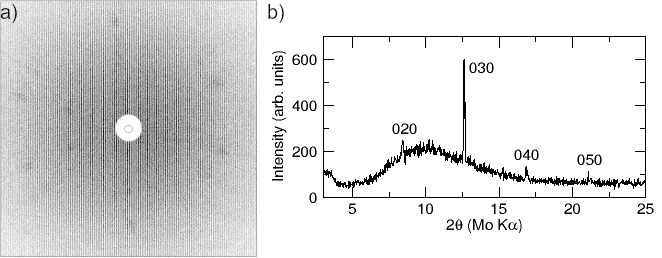
\includegraphics[width=\columnwidth]{figures/ch3/hex_CuMnAs_alignment.png} \\
\caption{\label{fig:hex_CuMnAs_alignment}
The two-fold symmetric Laue pattern obtained for \cumnas\ is shown in (a) and the reflective x-ray diffraction pattern for the same sample is shown is shown in (b).
}
\end{figure}

\subsection{SEM/EDS measurements}

% add brief statements about JEOL6060LV
Scanning electron microscopy (SEM) images were taken for all samples in the JEOL JSM-6060LV Low-Vacuum Scanning Electron Microscope. With proper beam alignment, astigmatism correction, wobble adjustment and focus, high quality images can be captured using this instrument. Using secondary electron detector, images can be obtained that gives information about the sample surface topology. Compositional as well as topological contrast can be obtained using back-scattered electrons. Energy dispersive x-ray microanalysis (EDX) were also carried out in the same instrument. EDX measures the energy of the characteristic x-rays emitted upon recombination of higher shell electrons of an element onto a hole in the lower shell.	This measurement can give quantitative information about the amount of elements present in the sample at a spot or a selected area.

\subsection{Calorimetry measurements}

% Discuss TGA, DSC and DTA

Thermogravimetric analysis (TGA) is a thermal analysis technique where the mass of the sample is tracked over a range of temperatures. It is particularly useful for detecting changes such as sublimation or evaporation of a phase or any kind of absorption/desoprtion processes. Powders or crystals of around 10~mg can be loaded onto an Alumina cup and heated up to 1000$^\circ$C for TGA. All the samples were measured in the Q50 TGA instrument upto above 400$^\circ$C under N$_2$ atmosphere to check if the sample loses its integrity at this temperature range or not. No transitions were observed in any of the samples measured and further analysis was carried out using differential scanning calorimetry (DSC). This measurement technique, although not very useful in this case, is necessary to prevent any accidental coating of the inner chamber during DSC measurements.

DSC is a calorimetry technique where the difference in the heat required to keep the sample at the same temperature as the reference is recorded as a function of temperature. It is a sensitive measurement technique and is useful for detecting magnetic transitions such as the N\'eel temperature or any spin canting transition. DSC measurements for all samples were carried out in the DSC2500 instrument. The sample powders, weighing between 4~mg to 8~mg, were loaded onto Alumina pans and subjected to heat-cool-heat cycles between -180$^\circ$C and 400$^\circ$ at 10$^\circ$C/min.

\begin{figure}
\centering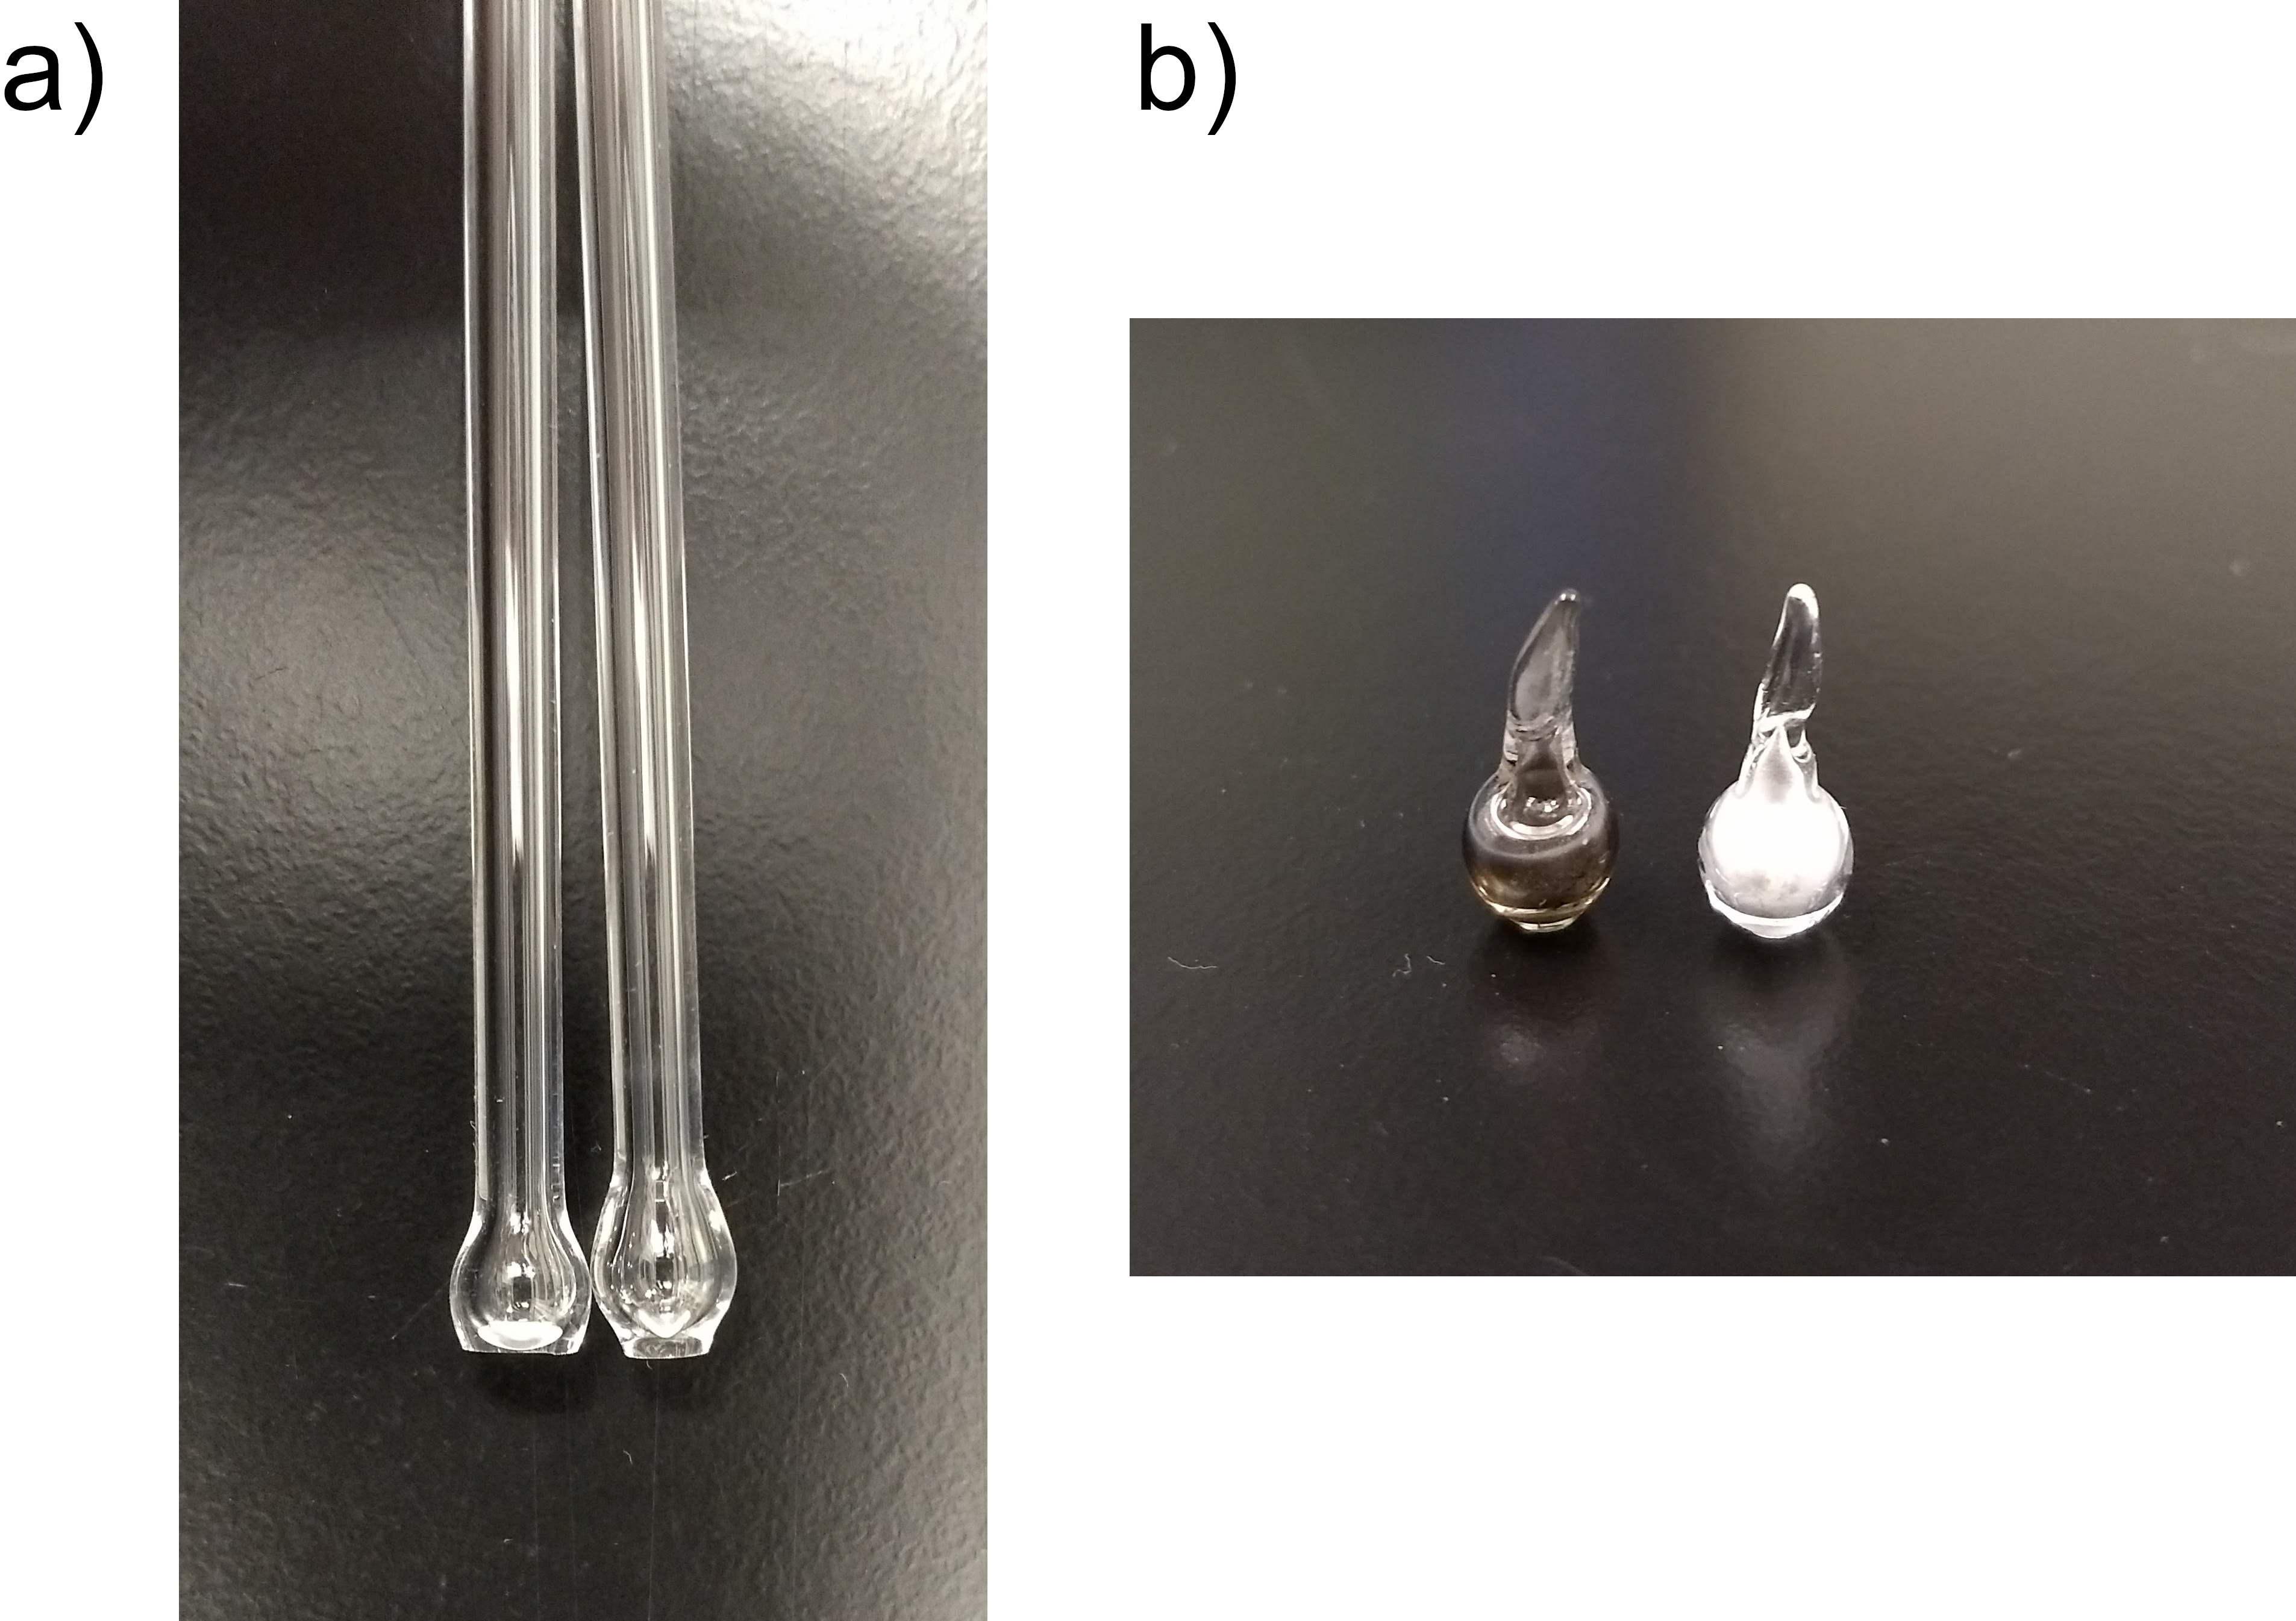
\includegraphics[width=0.6\columnwidth]{figures/ch3/DTA_tubes_combined.jpg} \\
\caption{\label{fig:DTA_tubes_combined}
The flat-bottom bulk of the quartz ampoules is shown in (a) and (b) shows the final powder-containing vacuum sealed ampoules.
}
\end{figure}

Differential thermal analysis (DTA) is similar to DSC except that the temperature difference between the sample and reference is recorded for identical thermal cycles. DTA measurements were carried out on a Shimadzu DTA-50 up to 1200$^\circ$C in some samples at a heating rate of 20$^\circ$C/min under N$_2$ atmosphere. The advantage of using DTA is that it can go up to very high temperatures which is useful for detecting melting point and any other phase transition that is beyond the range of DSC. The presence of As in the samples makes it impossible to use the standard DTA Alumina cups for measurement. To prevent contamination of the room with As vapors, special quartz ampoules were designed and commissioned from the SCS Glass shop. The ampoules were made by cutting 3~mm and 4~mm OD quartz tubes in 85~mm lengths and creating a flat-bottom bulb of 5~mm diameter at one end of the tube as shown in Fig. \ref{fig:DTA_tubes_combined}(a). About 20~mg to 40~mg of sample powders were vacuum sealed in the quartz ampoules and similar amount of Alumina powder was sealed as reference as shown in Fig. \ref{fig:DTA_tubes_combined}(b). The use of quartz ampoules, however, prevents detection of subtle transitions such as magnetic transitions. Hence, DTA can be used in conjunction with DSC to identify all transition temperatures.

\subsection{SQUID magnetometry measurements}

% Discuss squid measurements
SQUID measurements for all the samples were carried out in a Quantum Design MPMS3 (Magnetic Property Measurement System) in the DC mode. The DC moment was tracked as a function of applied field as well as temperature. In magnetic hysteresis measurements, fields up to 10~kOe were applied across six quadrants to account for the initial magnetization curve. Field cooling measurements in this document refer to the application of magnetic field at 400~K followed by cooling of the sample. Zero field cooling measurements were carried out by first cooling the sample to 5~K in the absence of a field, followed by the application of an external field and then, heating the sample. The sample moment is measured at certain intervals across the temperature range. The SQUID measurements have been carried out for the powders of Fe$_2$As, Cu$_{0.82}$Mn$_{1.18}$As, tetragonal CuMnAs and Mn$_3$As$_2$, and the single crystals of Fe$_2$As and Cu$_{0.82}$Mn$_{1.18}$As. In case of powders,between 20~mg to 40~mg of powders were filled into a VSM powder sample holder inside the Ar atmosphere glovebox. This capillary was snapped onto a MPMS3 brass half tube sample holder and wrapped with a small amount of insulating tape to keep it fixed. For single crystal measurements, aligned samples were fixed on the MPMS3 Quartz Paddle Sample Holder using GE Varnish and later removed using ethanol.


\subsection{Magnetotransport measurements}

% Discuss PPMS measurements and wire bonding

Resistivity measurements for hexagonal Cu$_{0.82}$Mn$_{1.18}$As were carried out in a Quantum Design Physical Property Measurement System Dynacool equipment using the resistivity module. The fractured sample that was aligned using the Laue setup and reflective x-ray diffraction measurements in Fig. \ref{fig:hex_CuMnAs_alignment} was fixed to a sapphire substrate using GE Varnish. The substrate was attached to the resistivity puck using a double-sided Kapton tape. Contacts were made between the pads on the puck and the sample using a 25 $\mu$m Al wire wedge bonder as shown in Fig. \ref{fig:resistivity}. For all measurements, current was applied along [001] and magnetic field was applied along [100]. Longitudnal and transverse resistivity measurements were carried out at different applied fields and temperatures. The results of the magnetotransport measurements for \cumnas\  are described in Chapter 5.

\begin{figure}
\centering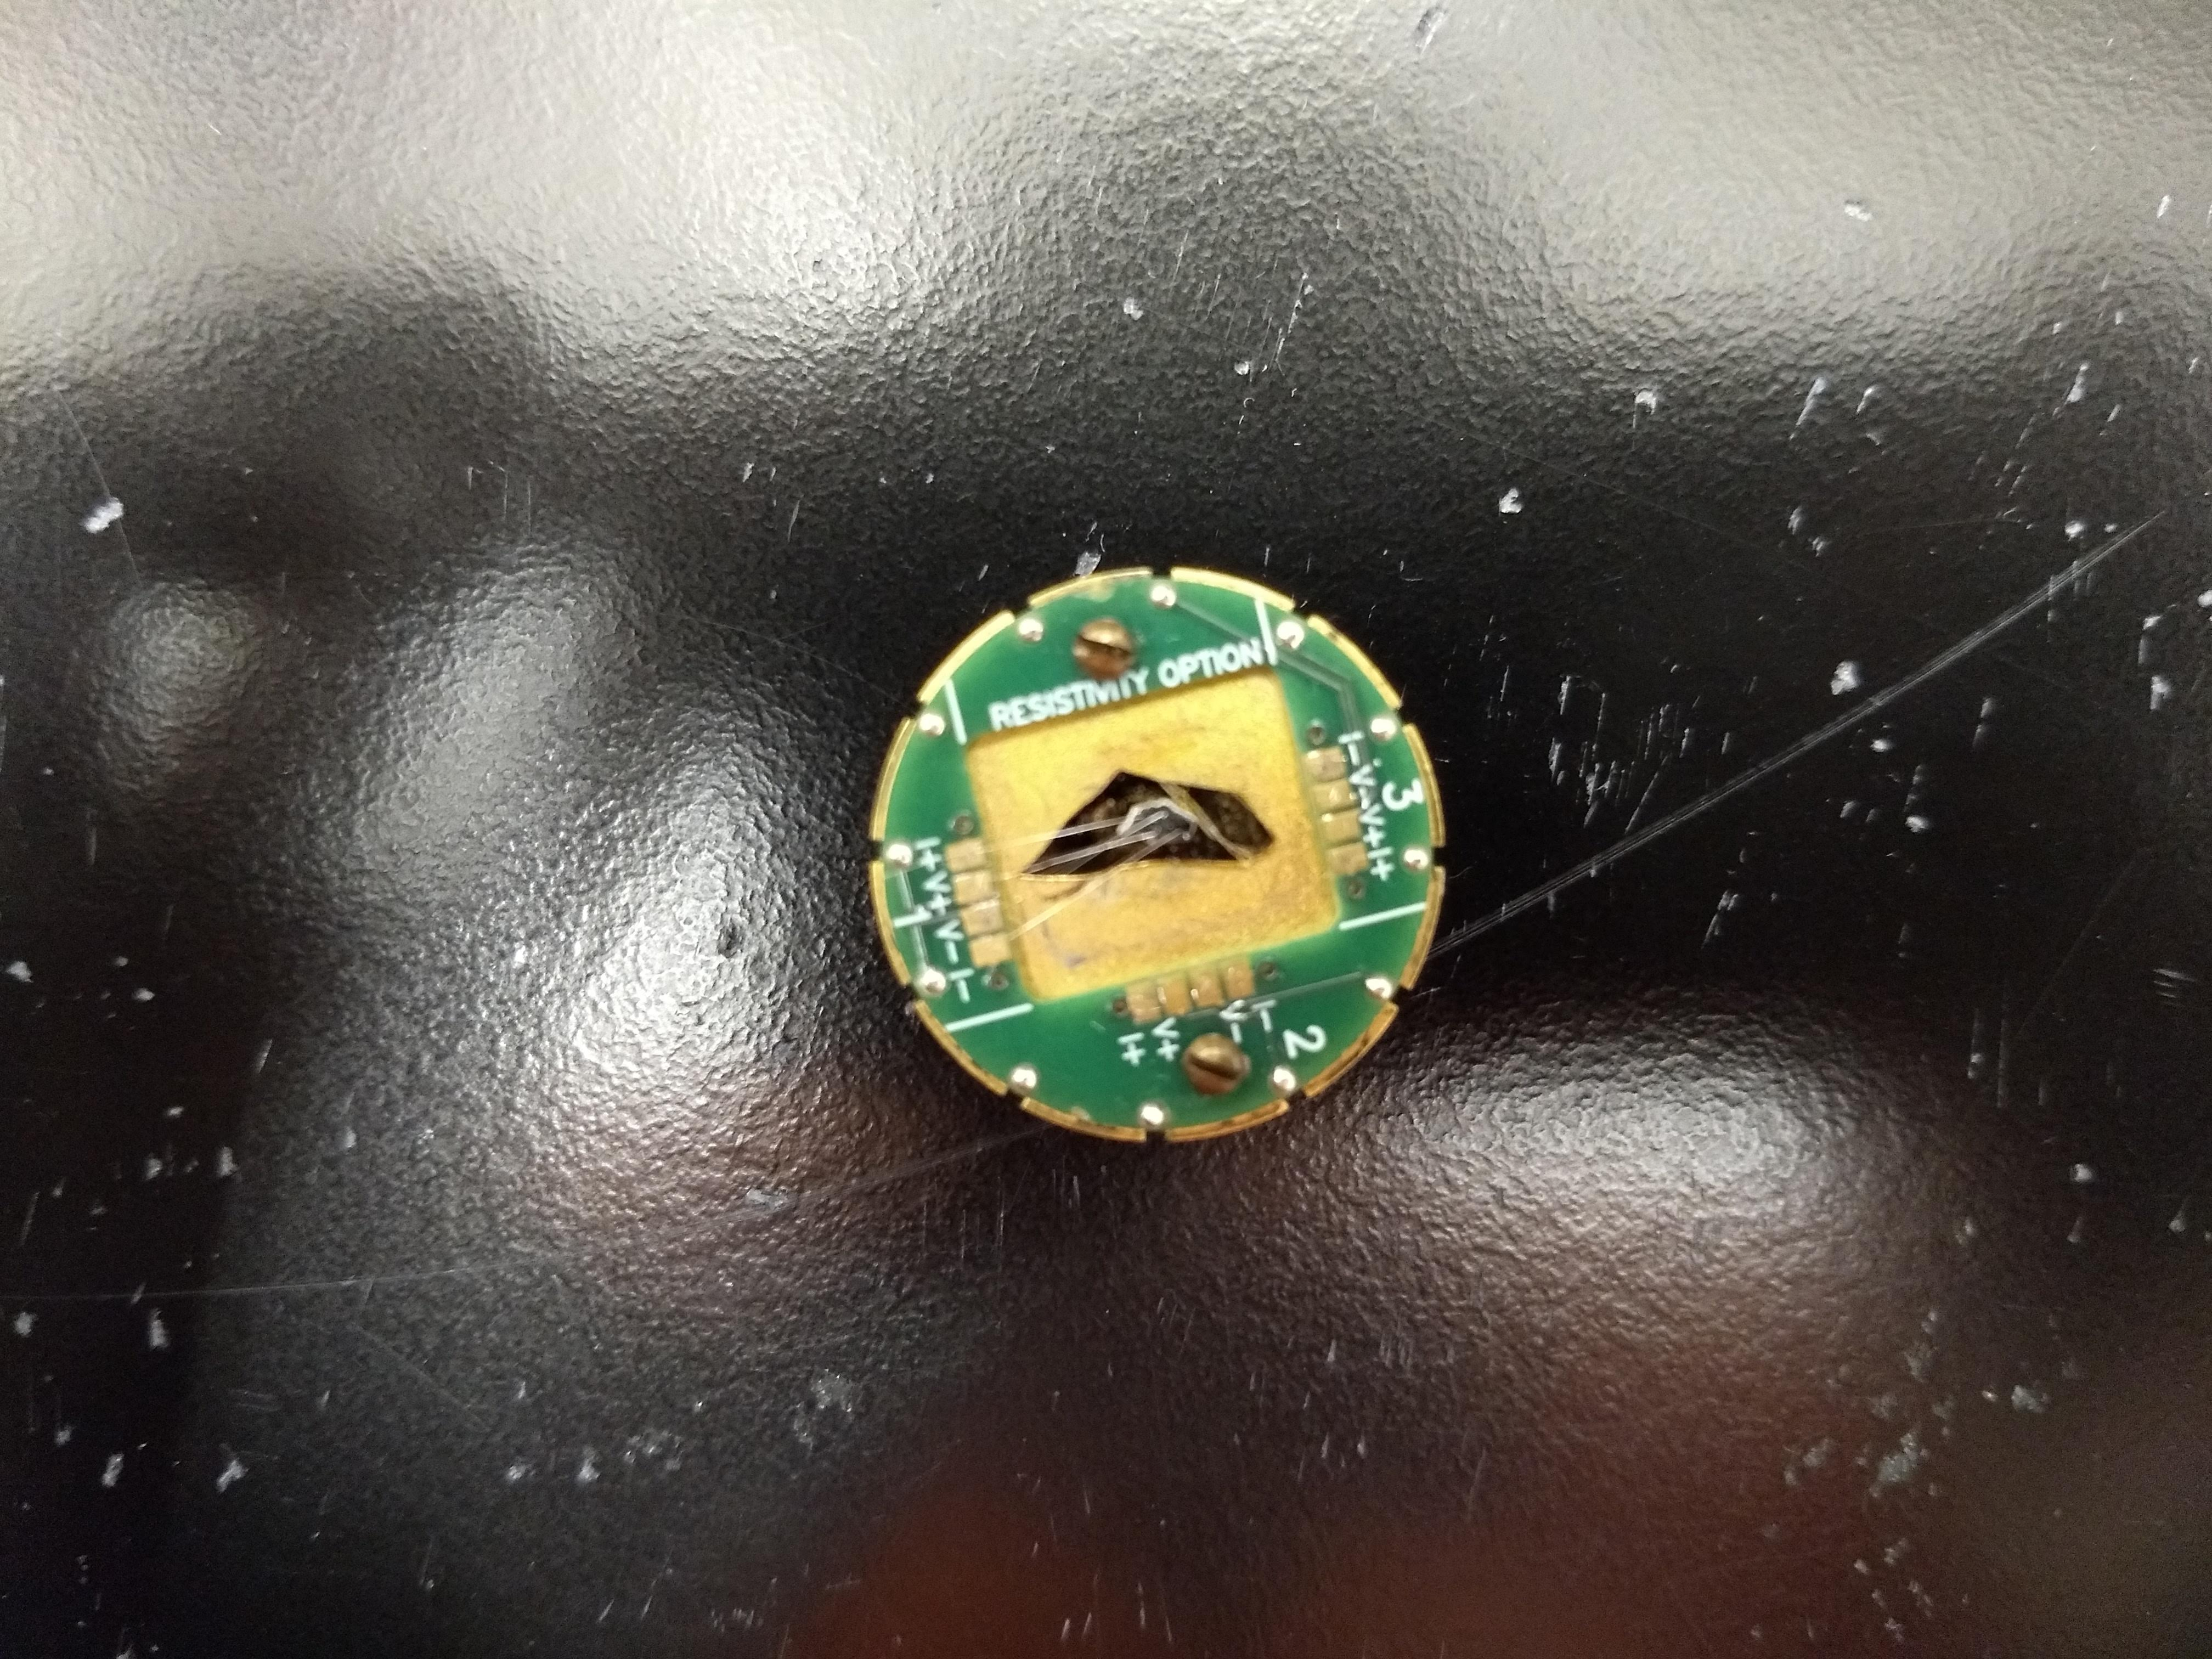
\includegraphics[width=0.5\columnwidth]{figures/ch3/resistivity.jpg} \\
\caption{\label{fig:resistivity}
Photo of the hexagonal \cumnas\ sample bonded to a resistivity puck for use in PPMS.
}
\end{figure}



\section{Neutron scattering}

Neutrons can be used as a probe from structural as well as magnetic characterization. Electrons contain charges and they interact strongly with matter and X-rays interact strongly with the electron cloud surrounding an atom. Neutrons, on the other hand, do not contain measurable electric dipole and weakly interact with matter. They can collide with the nucleus of an atom to provide structural information even in bulk materials. Unlike x-rays, there is no direct correlation between the atomic number of an element and its scattering cross section of neutrons. This helps in detecting light elements which is not possible using x-rays. Many dynamic processes such as lattice vibrations or spin waves occur at meV energy scales which is ideal to detect using neutrons. Since neutrons contain a finite magnetic moment, they can also interact with the dipole moment of an atom. Neutron diffraction is the only tool to extract the magnetic structure of a compound directly.

A neutron can either interact with the system as whole and interfere with other scattered neutrons resulting in coherent neutron scattering or interact with individual nuclei resulting in incoherent neutron scattering. In coherent scattering, when there is no energy transfer between the neutron and the system, the process is called elastic coherent scattering and neutron diffraction is the most famous example of this case. When there is an energy transfer between the neutron and the system, the process is inelastic coherent scattering and it gives information on various phonon and magnon modes present in the system. Neutron diffraction data looks very similar to x-ray diffraction data with two major exceptions. The form factor in the case of neutrons remain independant of the angle and neutrons also provide intensity from magnetic scattering. The nuclear and magnetic scattering contributions can be added independantly to provide the final neutron diffraction pattern.

\subsection{Neutron diffraction}

% Discuss different instruments and analysis

Neutron diffraction measurements reported in this document were carried out at various beamlines in Oak Ridge National Laboratory (ORNL). ORNL has two facilities where neutron scattering measurements can be carried out. The Spallation Neutron Source (SNS) produces neutrons by spallation of a target by protons that have been accelerated up to very high speeds. The neutrons ejected from the target are moderated down to an accepted temperature and sent to various beamlines. Instruments in this facility can make use of time-of-flight techniques to get information on the neutron energy and momentum. High Flux Isotope Reactor (HFIR) provides steady-state flux of neutrons through nuclear reaction. Using monochromators at source and detector side, high resolution can be obtained for a narrow Q-range. Neutron powder diffraction (NPD) for most samples were carried out at the NOMAD and POWGEN beamlines in SNS. NPD of \cumnas\ was measured at the WAND$^2$ beamline and single crystal neutron diffraction of \cumnas\ was measured at HB-3A beamline in HFIR. In addition, tetragonal CuMnAs and Mn$_3$As$_2$ samples were also shipped to Australian Centre for Neutron Scattering for NPD measurements at WOMBAT and ECHIDNA beamlines. WOMBAT beamline also allows single crystal neutron diffraction measurements and ECHIDNA is ideal for carrying out high resolution NPD measurements. Methods of obtaining the magnetic structure from NPD data will be discussed in the next chapter.


\subsection{Inelastic neutron scattering}

%Discuss ARCS instrument

In inelastic neutron scattering (INS) measurements, the energy and momentum of the incoming and scattered neutrons are tracked to give information about the dynamic structure factor. The precise nature in which this is done differs from one instrument to another. The incident neutron may give or receive energy from the system and the total energy of the system plus neutron must be conserved. The INS measurements for Fe$_2$As single crystals were carried out in the ARCS beamline at the Spallation Neutron Source (SNS). ARCS is a time-of-flight chopper neutron spectrometer with a wide angular coverage, ideal for gathering complete INS spectra of Fe$_2$As. Thermal neutrons coming from the moderator go through a series of choppers before reaching the sample. T0 chopper removes unwanted neutrons and other radiations from the beam and defines the starting time for the neutrons. The Fermi choppers select neutrons having particular incident neutron energies. The intial momentum and energy of neutrons are known. The time taken by the neutron to reach the detector determines the final energy of the neutron and its position in the detector determines its final momentum. Both single crystals and powders can be used in the ARCS beamline for INS measurements. 5 crystals of Fe$_2$As were co-aligned using a Laue setup at SNS.

The final data obtained from the INS experiment is four dimensional (3 $Q$-axes and an energy axis) in nature and requires a huge amount of memory to store and process. The data can be reduced to lower dimensions by integrating it along one, two or three axes. The conventional INS spectra that we usually see in manuscripts is Energy vs $Q$ or constant energy slices where the other two axes have been integrated over a finite width. This action can be performed by writing python scripts and running it using \textsc{mantid}. Once the data is reduced, it can saved as a text file for easier processing on personal computers. A complete 360$^\circ$ scan in the ARCS instrument typically takes 24-36 hours. Cutting and slicing data correctly and being able to analyze this data within this timeframe is crucial to determine the next steps during beamtime.

Simulated magnon spectra can be plotted using \textsc{SpinW}. Once we define out crystal, we have to define various exchange pathways for consideration. We can then assign exchange coupling values to these pathways. Magnetic anisotropy of the crystal can also be accounted in \textsc{SpinW}. There are provisions for switching between the calculated and simulated magnon spectra. To get a simulated magnon spectra that matches close to the experiment, one can calculate the magnon spectra at different points across the finite width of integration and sum or average all the intensities. It is also possible to refine exchange coupling constants from the experimental magnon spectra in \textsc{SpinW}. The experimental data points have to manually inserted in a certain format for a every value of $Q$. There are few parameters that can be tuned during refinement such as the minimum and maximum values of exchange constants, the optimizer used for refinement, the Hamiltonian being used during refinement etc. In the INS measurement of Fe$_2$As, we simulate magnon spectra from previous computationally calculated values and also refine the experimental spectra to obtain exchange coupling constants.

%##################chapter 4
\chapter{Magnetic structure refinement from neutron diffraction measurements}

\begin{figure}
\centering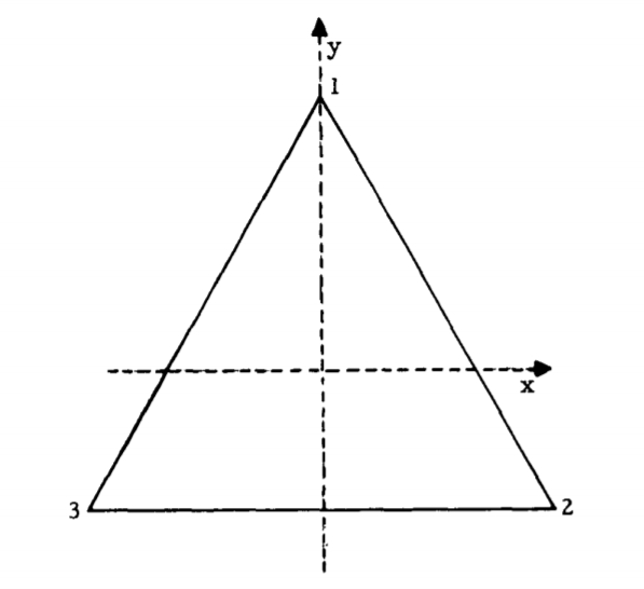
\includegraphics[width=0.5\columnwidth]{figures/ch4/C3v.png} \\
\caption{\label{fig:C3v}
Electronic band structure
}
\end{figure}

\begin{figure}
\centering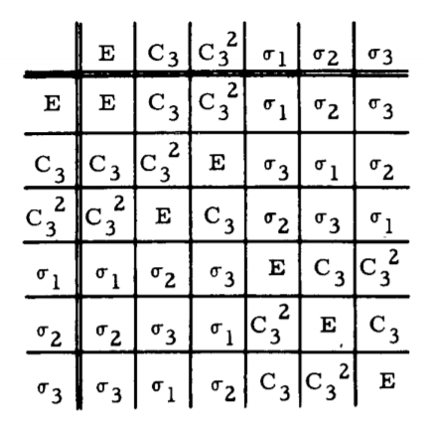
\includegraphics[width=0.5\columnwidth]{figures/ch4/group_multiplication_table_C3v.png} \\
\caption{\label{fig:gmt_C3v}
Electronic band structure
}
\end{figure}

\begin{figure}
\centering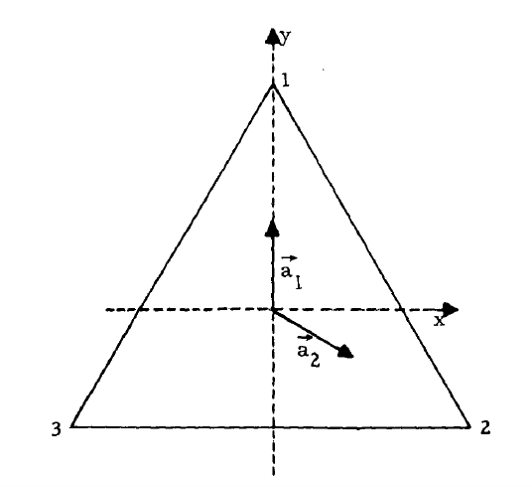
\includegraphics[width=0.5\columnwidth]{figures/ch4/C3v_a1_a2.png} \\
\caption{\label{fig:C3v_a1_a2}
Electronic band structure
}
\end{figure}

\begin{figure}
\centering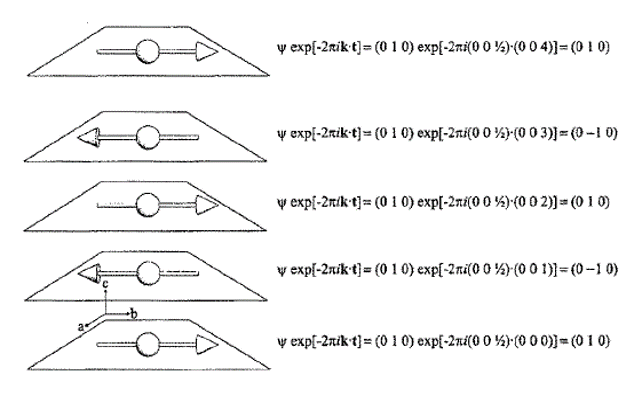
\includegraphics[width=\columnwidth]{figures/ch4/propagation_vector.png} \\
\caption{\label{fig:propagation_vector}
Electronic band structure
}
\end{figure}

\begin{figure}
\centering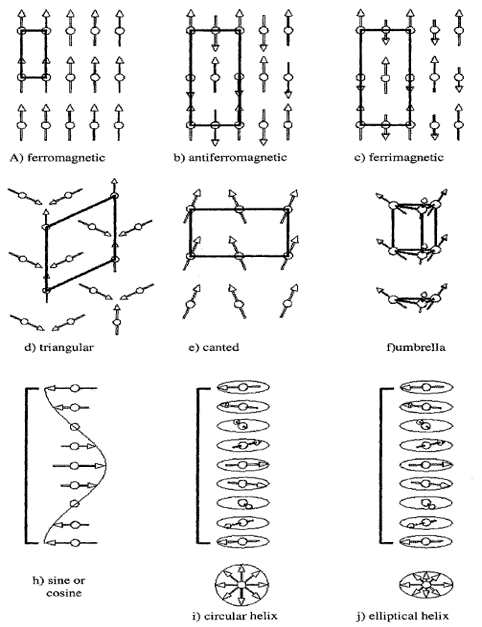
\includegraphics[width=\columnwidth]{figures/ch4/mag_structures_single_k.png} \\
\caption{\label{fig:mag_structures_single_k}
Electronic band structure
}
\end{figure}

\begin{figure}
\centering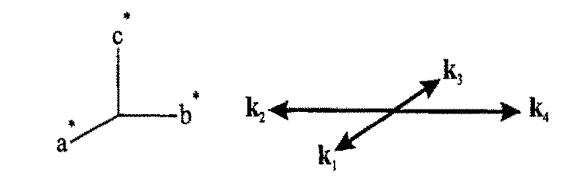
\includegraphics[width=0.7\columnwidth]{figures/ch4/star_of_propagation_vector_k.png} \\
\caption{\label{fig:star}
Electronic band structure
}
\end{figure}

\begin{figure}
\centering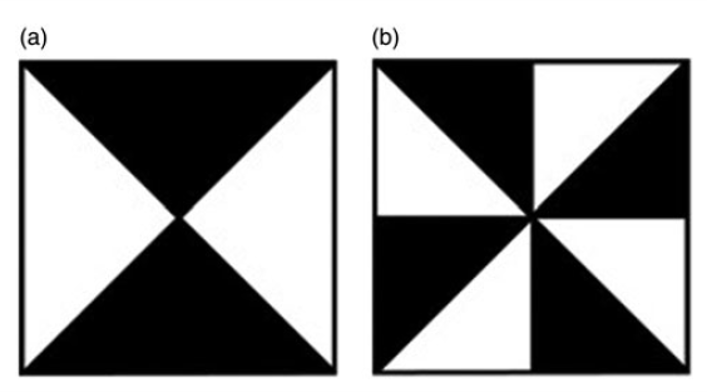
\includegraphics[width=0.5\columnwidth]{figures/ch4/symmetry_based_analysis.png} \\
\caption{\label{fig:symmetry_based_analysis}
Electronic band structure
}
\end{figure}

\Blindtext[6]


%##################chapter 5
\chapter{An in-plane hexagonal antiferromagnet in the Cu-Mn-As system, Cu$_{0.82}$Mn$_{1.18}$As}

%\section{Copyrights and author contributions}

\hfill \break

\href{https://doi.org/10.1103/PhysRevMaterials.3.111402}{Reprinted with permission from Manohar H. Karigerasi, Kisung Kang, Arun Ramanathan, Danielle L. Gray, Matthias D. Frontzek, Huibo Cao, Andr\'e Schleife, and Daniel P. Shoemaker, Physical Review Materials 3, 111402(R) (2019). Copyright 2020 by the American Physical Society.} In this work, I synthesized single crystals and powders of \cumnas, analyzed neutron diffraction and synchrotron x-ray difraction data and carried out SQUID and magnetotransport measurements. Kisung Kang did DFT simulations to verify the magnetic ground state of \cumnas\ and obtain the band structure. Arun Ramanathan also synthesized the samples. I wrote the paper with help from the coauthors.

%\iffalse
%\begin{abstract}

\section{Abstract}
We report the single-crystal growth and characterization of a new hexagonal phase, Cu$_{0.82}$Mn$_{1.18}$As, in the Cu-Mn-As system. 
This compound contains the same square-pyramidal MnAs$_5$ units as the tetragonal and orthorhombic polymorphs of CuMnAs.
Calorimetry, magnetometry, and neutron diffraction measurements reveal antiferromagnetic ordering at 270~K.
The magnetic structure consists of a triangular arrangement of spins in the $ab$ plane. 
Hexagonal Cu$_{0.82}$Mn$_{1.18}$As shows resistivity that varies only weakly from 5~K to 300~K, and is many times higher than tetragonal CuMnAs, indicative of a strongly-scattering metal.
First-principles calculations confirm the metallic band structure with a small density of states at the Fermi energy. The neutron-refined
magnetic ground state is close to the computationally-determined minimum energy configuration. This compound should serve as a clear control when disentangling the effects of current-driven N\'{e}el switching of metallic antiferromagnets since it exhibits in-plane spins but the magnetic ordering does not break degeneracy along the $a$ and $b$ directions, unlike tetragonal CuMnAs.
%\end{abstract}

%\fi

\section{Introduction} 

Recent demonstrations on electronic switching of domains in  semimetallic tetragonal CuMnAs have attracted considerable interest in the field of antiferromagnetic (AF) spintronics \cite{Wadley2016,Grzybowski2017,Wadley2018,Matalla-Wagner2019}. Thin films of tetragonal CuMnAs grown on GaP (001) substrates have a N\'eel temperature $T_N$ of about 480 K \cite{Wadley2015,Hills2015}.
These studies are complicated by the variable allowed stoichiometries of  phases in the Cu--Mn--As system.
Before any domain-switching studies were demonstrated, bulk tetragonal CuMnAs was shown to be 
stabilized by the addition of excess nominal Cu in solid-state reactions \cite{Uhlirova2015}.
A large variation in the N\'{e}el temperature $T_N$ from 507~K to 320~K has been shown as Cu excess in Cu$_{1+x}$Mn$_{1-x}$As increases from $x = 0.02$ to 1.4 \cite{Uhlirova2019}, and a weak ferromagnetic transition around 300~K was reported around $x=0$ \cite{Nateprov2011}.
On the Mn excess side, orthorhombic CuMn$_3$As$_2$ is formed as a stable phase \cite{Uhlirova2015}.
 
When Cu, Mn, and As are mixed stoichiometrically, CuMnAs crystallizes in an orthorhombic $Pnma$ phase \cite{MacA2012}.
Orthorhombic CuMnAs is the first compound to have been proposed as a magnetically-ordered Dirac semimetal \cite{Tang2016} and has been discussed for the possibility of voltage-induced switching \cite{Kim2018}.
Initial characterization by M\'{a}ca \emph{et al.}\ showed $T_N = 360$~K as judged by resistivity and differential thermal analysis \cite{MacA2012}. This commensurate magnetic ordering and $T_N$ in orthorhombic CuMnAs was confirmed by Emmanouilidou \emph{et al.}, who also found that a slightly cation deficient tetragonal sample Cu$_{0.98}$Mn$_{0.96}$As exhibits an incommensurate AF ordering at 320~K, followed by another AF reorientation around 230~K \cite{emmanouilidou_magnetic_2017}.

\begin{figure}
\centering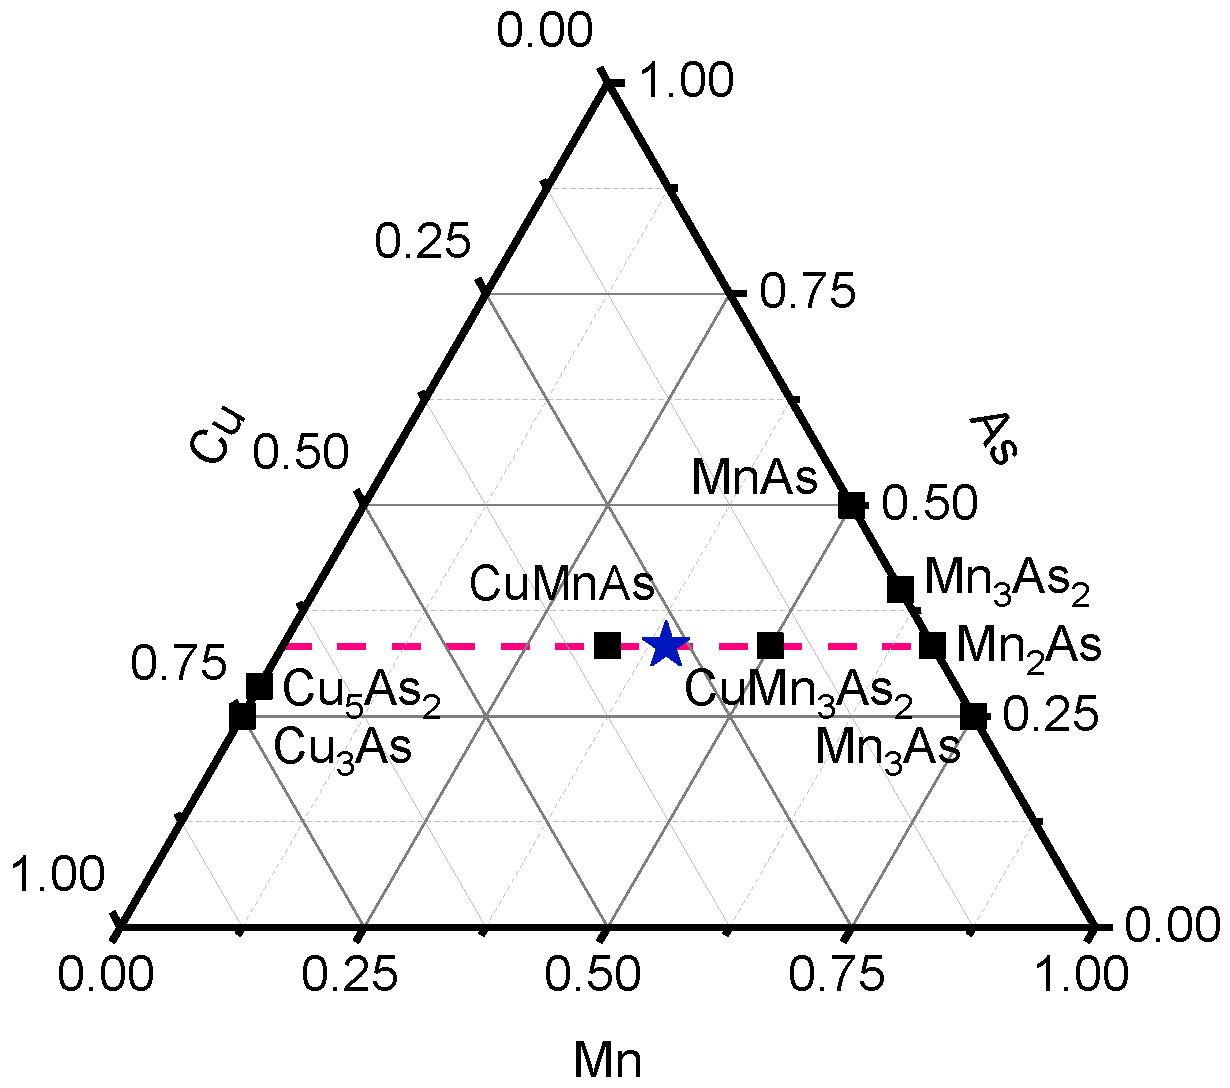
\includegraphics[width=0.6\columnwidth]{figures/ch5/phase_diagram_cropped.pdf} \\
\caption{\label{fig:phase_diagram}
{\color{black}Hexagonal Cu$_{0.82}$Mn$_{1.18}$As has been marked with a star among the previously-known phases in the Cu--Mn--As system. Compositions near CuMnAs are known to crystallize in both tetragonal and orthorhombic crystal systems.}
} 
\end{figure}

{\color{black} All known ternary phases in the Cu--Mn--As system have the transition metal ($M$) to As ratio of 2:1 and are either tetragonal or orthorhombic as shown in Fig.\ \ref{fig:phase_diagram}.}
The metallic nature of these compounds allows significant deviation from $M_2$As stoichiometry, as evidenced by the binary compounds MnAs (a ferromagnet with a reentrant FeP-to-NiAs-type transition) \cite{Pytlik1985,Schwartz1971,Glazkov2003}, Mn$_3$As$_2$ (which has at least three polymorphs)\cite{Dietrich1990,Moller1993,Hagedorn1994}, the seemingly metastable compounds Mn$_4$As$_3$ and Mn$_5$As$_4$ \cite{Hagedorn1995,Moller1993}, and Mn$_3$As \cite{nowotny_kristallchemische_1951}.
Of these compounds, only MnAs and Mn$_2$As have been investigated with neutron diffraction and transport measurements \cite{Yuzuri1960,Austin1962}.
Further elaboration of compounds in this space is necessary to understand the potential for manipulating spins in these highly-correlated phases.

\section{Methods}

Millimeter-sized crystals of hexagonal \cumnas\ were synthesized by mixing elemental powders Cu (99.9\% metals basis), Mn (99.98\% metals basis), and As (99.9999\% metals basis) in 0.82:1.18:1 molar ratio. 
The powders were vacuum sealed in quartz tubes and heated at 1$^\circ$C/min to 600$^{\circ}$C for 6 hours then ramped at 1$^{\circ}$C/min to 975$^{\circ}$C for 1 hour. The tube was slow cooled at 1$^{\circ}$C/min to 900$^{\circ}$C and held for 1 hour before furnace-cooling down to room temperature. The resulting product was a solid ingot. The ingot was crushed into smaller pieces to conduct single crystal X-ray diffraction on a Bruker X8 Apex II diffractometer at 296~K and $\lambda = 0.71073$~\AA. 


Variable-temperature powder X-ray diffraction was performed using a nitrogen blower at beamline 11-BM of the Advanced Photon Source in Argonne National Laboratory ($\lambda = 0.4128$~\AA) \cite{wang_dedicated_2008}. Variable-temperature neutron powder diffraction was conducted at the WAND$^2$ instrument at the High-Flux Isotope Reactor (HFIR) at Oak Ridge National Laboratory \cite{Frontzek_new}.


Magnetic structure determination was performed on a 2~mm crystal at the HB-3A four circle diffractometer at HFIR. A total of 344 reflections were collected at 4~K and used for structural refinement. Magnetic symmetry analysis was carried out using the tools available at the Bilbao Crystallographic Server \cite{Perez-Mato2015}
and refined using the FullProf suite \cite{rodriguez-carvajal_recent_1993}.

Differential scanning calorimetry (DSC) measurements were performed on 5~mg of powder in Al pans under N$_2$ atmosphere in a TA Instruments DSC 2500. A small fractured sample, weighing about 12 mg, was polished and aligned using Laue diffraction. This sample was mounted onto a quartz paddle sample holder for aligned magnetometry measurements in a Quantum Design MPMS3. Aligned resistivity measurements were carried out using the 4-point probe method in a Quantum Design PPMS DynaCool.

First-principles density functional theory (DFT) simulations were performed using the Vienna \emph{Ab-Initio} Simulation Package  (VASP) \cite{Kresse:1996,Kresse:1999}. The electron-ion interaction is described using the projector-augmented wave (PAW) scheme \cite{Blochl:1994}. Exchange and correlation are described using the generalized-gradient approximation (GGA) by Perdew, Burke, and Ernzerhof  (PBE) \cite{Perdew:1997}. Single-particle Kohn-Sham states are expanded into a plane-wave basis with a cutoff energy of 600 eV. Monkhorst-Pack \cite{Monkhorst:1976} (MP) $\mathbf{k}$-point grids of $2\,\times\,2\,\times\,6$ and $4\,\times\,4\,\times\,12$ are used to integrate the Brillouin zone for cell relaxation and electronic band structure calculations, respectively.
Non-collinear magnetism and spin-orbit coupling is taken into account in all calculations \cite{Steiner2016}.
Self-consistent total-energy convergence was achieved to within $10^{-6}$ eV and atomic positions were relaxed until Hellman-Feynman forces were smaller than 5~meV/\AA.

\section{Results and Discussion}

\subsection{Structure refinement}

\begin{figure}
\centering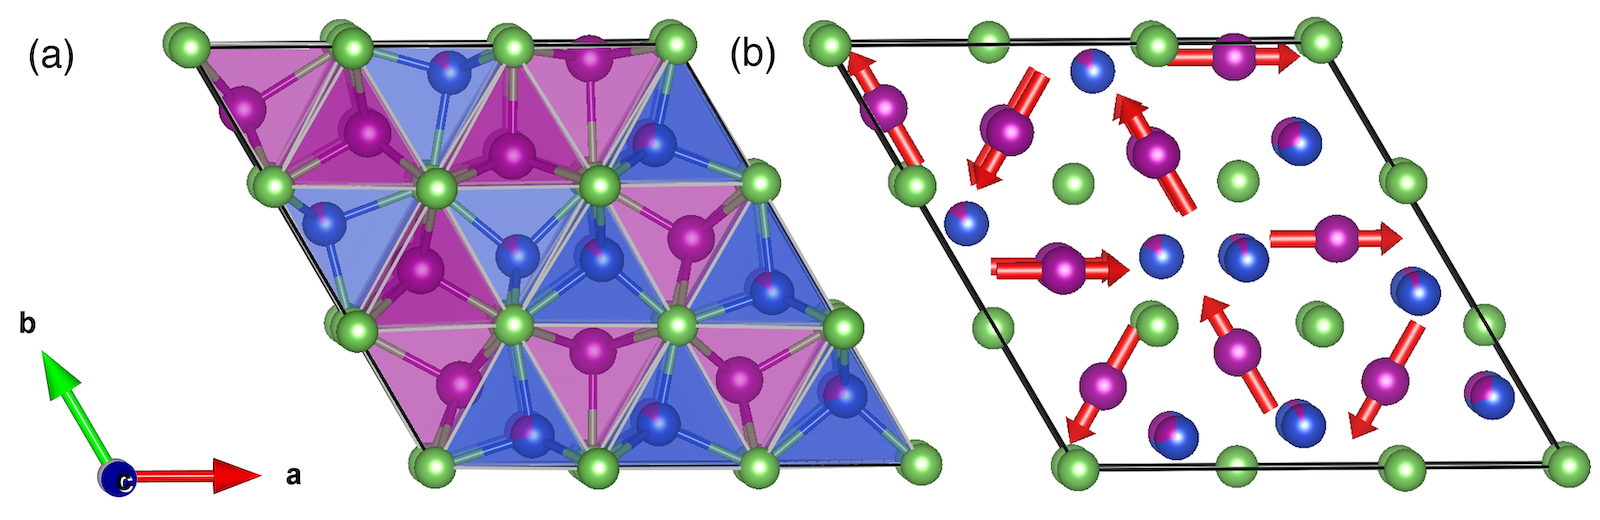
\includegraphics[width=\columnwidth]{figures/ch5/h-cumnas_1x1_cells_v2.png} \\
\caption{\label{fig:unitcell}
Unit cell of Cu$_{0.82}$Mn$_{1.18}$As (a) is shown with square pyramidal Mn in purple, tetrahedrally coordinated Cu in blue, and As in green.
In (b), the refined magnetic structure is shown with moments on the Mn sites.
} 
\end{figure}

The refined structure of \cumnas\ is shown in Fig.\ \ref{fig:unitcell}(a), with structural parameters from single-crystal X-ray diffraction (XRD) given in Table \ref{tab:sxtl} and \ref{tab:atoms}.
{\color{black}\cumnas\ has a short lattice parameter $c \approx 3.8$~\AA, indicating that the unit cell is flat and is the same width as the Cu and Mn coordination polyhedra. Fig.\ \ref{fig:unitcell}(a) shows the unit cell viewed down $c$, with all the atoms occupying either $z$ = 0 or $z$ = 0.5.}
The compound forms in a new structure type with space group $P\overline{6}$, and is comprised of three inequivalent square-pyramidal Mn and three inequivalent tetrahedral Cu, all coordinated by As.
All metal sites have a multiplicity of 3 {\color{black} and have $m$ point symmetry}. The atomic positions are well-described by the single-crystal XRD data, but the occupancies are less reliable due to the similar electron densities at each site.  
High-resolution synchrotron powder X-ray diffraction is shown in Fig.\ \ref{fig:xrd-neutron}(a), to confirm that these samples can be made highly pure with excellent crystallinity.

The occupancies are better constrained by neutron scattering, where Mn and Cu have more contrast in their scattering lengths ($-3.73$ and 7.718 fm, respectively) \cite{sears_neutron_1992}.
Neutron powder diffraction data from WAND$^2$ were collected at 400~K, in the paramagnetic regime, with the refinement shown in Fig.\ \ref{fig:xrd-neutron}(b). 
No evidence for site mixing or vacancies on the Mn or As sites was apparent. 
The best refinements were obtained by using the nominal Cu/Mn ratio and allowing Mn mixing on the Cu sites, with the final Cu occupancies of 0.709(2), 0.914(3), and 0.846(2) for Cu sites 1\,--\,3, respectively.
The final structural refinement data presented in Table \ref{tab:atoms} is a single-crystal XRD refinement with the occupancies locked to values obtained by co-refinement to the 100~K synchrotron X-ray and 400~K neutron scattering data. 

\begin{figure}
\centering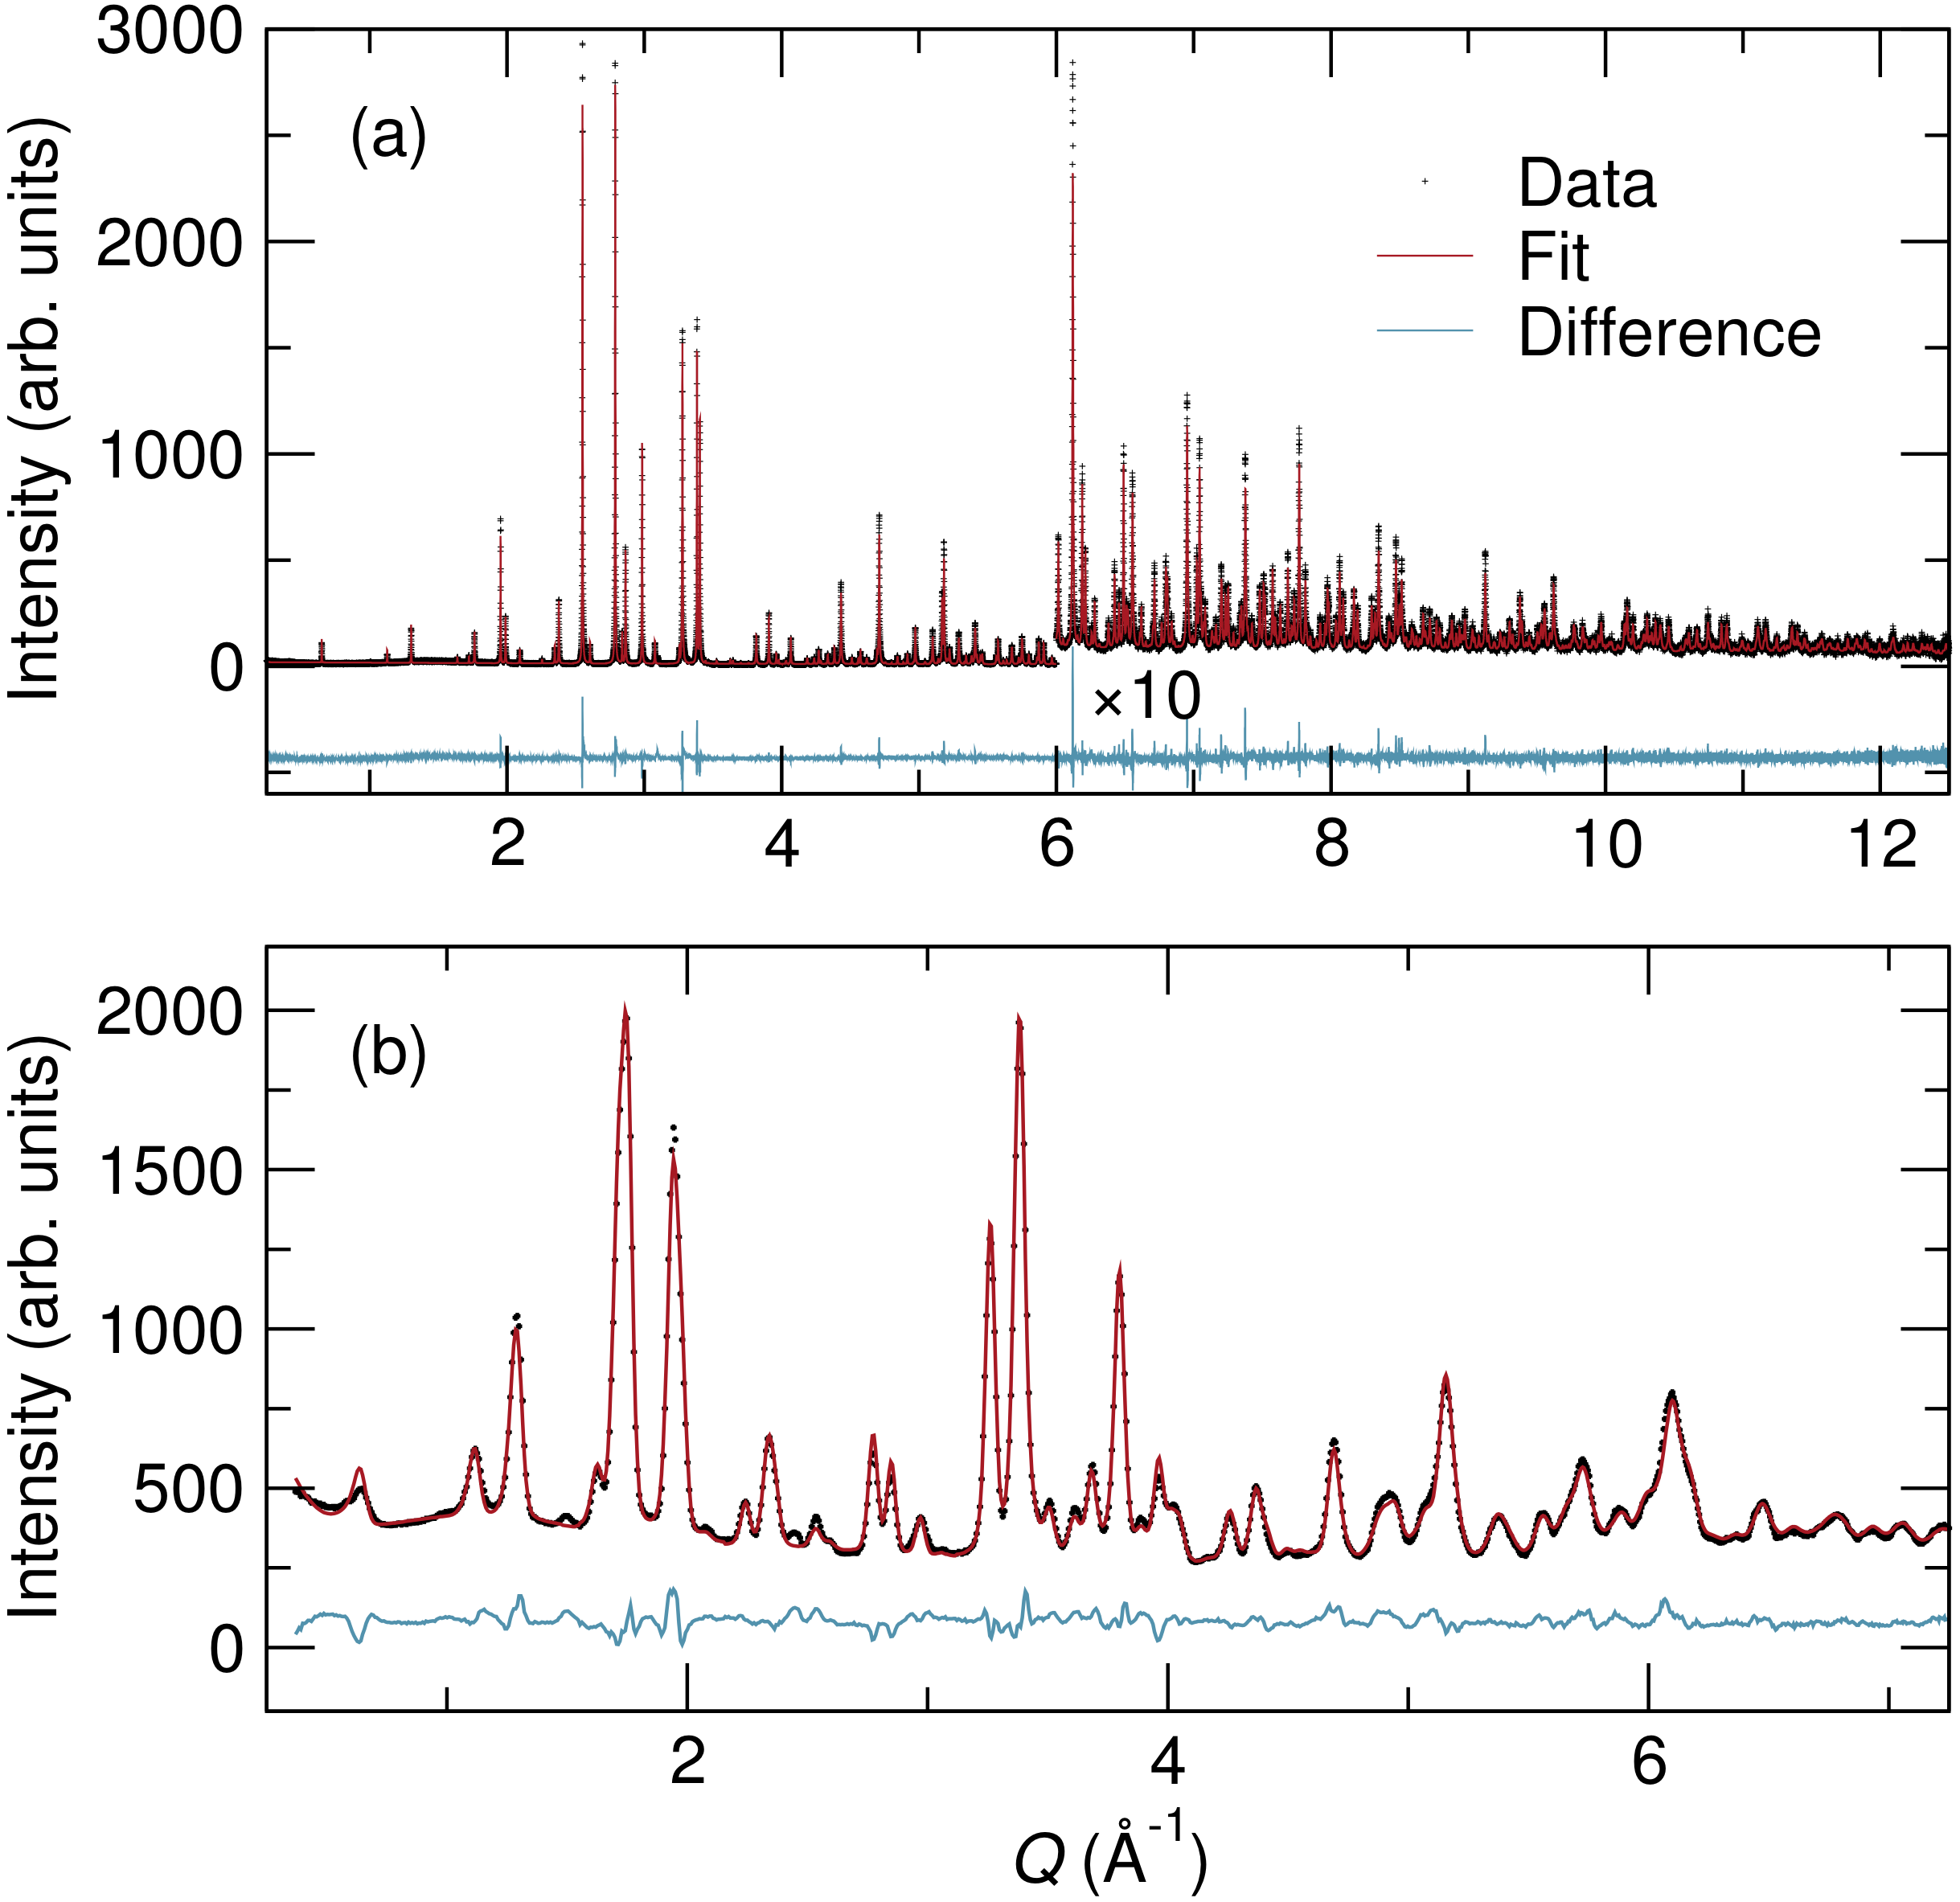
\includegraphics[width=0.7\columnwidth]{figures/ch5/h-cumnas_11bm_100k_wand_400k_combine} \\
\caption{
Refinements of Cu$_{0.82}$Mn$_{1.18}$As to (a) synchrotron X-ray powder diffraction at 100~K at APS 11-BM ($\lambda = 0.4128$~\AA) and (b) neutron powder diffraction at 400~K on WAND$^2$ ($\lambda = 1.487$~\AA).
}
\label{fig:xrd-neutron}
\end{figure}

\begin{comment}
Cu occupancies from 100 K 11-BM:
H-CUMNAS_11BM_100K_WAND-OCC.LST
                     frac       x         y         z     100*Uiso  100*U11  100*U22  100*U33  100*U12  100*U13  100*U23
 CU    (  1) Values  : 0.880  0.421107  0.504842  0.500000    0.247
             Sigmas  : 0.005  0.000349  0.000247              0.015
             Shft/esd:  0.34     -0.28      0.41              -0.01
 Cu1      moved  0.00A     sum(shift/e.s.d)**2 :    0.36

 CU    (  2) Values  : 0.799  0.251052  0.087549  0.000000    0.247
             Sigmas  : 0.004  0.000407  0.000430              0.015
             Shft/esd: -0.19      0.38      0.27              -0.01
 Cu2      moved  0.00A     sum(shift/e.s.d)**2 :    0.25

 CU    (  3) Values  : 0.976  0.588831  0.504290  0.000000    0.247
             Sigmas  : 0.004  0.000338  0.000191              0.015
             Shft/esd: -0.30     -0.48      0.63              -0.01
 Cu3      moved  0.00A     sum(shift/e.s.d)**2 :    0.71
 
 
 Cu occupancies from 400 K WAND2:
 P-6_WAND2_400K_REFINE.LST
  Atom parameters for phase no. 1
                      frac       x         y         z     100*Uiso  100*U11  100*U22  100*U33  100*U12  100*U13  100*U23
 CU    (  1) Values  : 0.723  0.421100  0.503100  0.500000    1.515
             Sigmas  : 0.019                                  0.065
             Shft/esd: -5.13                                  -0.28
 Cu1      moved  0.00A     sum(shift/e.s.d)**2 :   26.37

 CU    (  2) Values  : 0.622  0.248900  0.085800  0.000000    1.515
             Sigmas  : 0.014                                  0.065
             Shft/esd:  2.48                                  -0.28
 Cu2      moved  0.00A     sum(shift/e.s.d)**2 :    6.23

 CU    (  3) Values  : 0.943  0.589400  0.504100  0.000000    1.515
             Sigmas  : 0.017                                  0.065
             Shft/esd:  3.19                                  -0.28
 Cu3      moved  0.00A     sum(shift/e.s.d)**2 :   10.22
\end{comment}


\begin{table}
\caption{\label{tab:sxtl} 
Structural parameters obtained from room-temperature Mo-$K\alpha$ X-ray
single-crystal refinement (full-matrix least-squares on $F^2$) with occupancies fixed from synchrotron X-ray and neutron co-refinement. 
}
\centering
\begin{tabular}{ll}
\hline
Formula								&  \cumnas\ \\
Formula Weight						& 191.88 g/mol\\
Crystal system						& Hexagonal \\
Space group							& $P\overline{6}$\\
$a=b$									& 11.1418(3) \AA \\
$c$									& 3.8311(2) \AA \\
$V$, $Z$ 								& 411.87(3) \AA$^3$, 9 \\
$\rho$ 								& 6.962 g/cm$^3$ \\
Absorption coefficient			& 35.046 mm$^{-1}$ \\
$F$(000) 							& 777 \\ 
$(\sin\theta/\lambda)_{max}$ 					& 0.714 \\
Reflections collected       	& 6722 \\
Observed $I>2\sigma(I)$ reflections       	& 953 \\
$R_{int}$							& 0.0682 \\
Number of parameters 			& 56 \\
Goodness-of-fit on $F^2$		& 1.445 \\
$R[F^2 > 2\sigma(F^2)], wR(F^2)$    &   0.0344, 0.0849 \\
\hline
\end{tabular}
~\\
\end{table}

\begin{sidewaystable}
\caption{\label{tab:atoms} 
Atomic parameters obtained from room-temperature X-ray single-crystal refinement of Cu$_{0.82}$Mn$_{1.18}$As.
Occupancy values for Cu/Mn sites are co-refined to 100~K synchrotron and 400~K neutron powder diffraction data (see Fig.\ \ref{fig:xrd-neutron}).
Atomic displacement parameters $U_{ij}$ are given in units of \AA$^2$.
}
\centering
\begin{tabular}{p{1.7cm}p{0.9cm}p{1.7cm}p{1.7cm}p{0.9cm}p{2.3cm}p{1.7cm}p{1.7cm}p{1.7cm}p{1.7cm}}
\hline\hline
Atom	 & Site	 & $x$	 & $y$	 & $z$	 & Occupancy	 & $U_{11}$	 & $U_{22}$	 & $U_{33}$	 & $U_{12}$\\
\hline
Cu1/Mn1	 & 3j	 & 0.2489(9)	 & 0.0868(10)	 & 0	 & 0.709/0.291(2)	 & 0.025(3)	 & 0.023(4)	 & 0.030(3)	 & 0.014(2)\\
Cu2/Mn2	 & 3j	 & 0.5894(9)	 & 0.5043(5)	 & 0	 & 0.914/0.086(3)	 & 0.012(3)	 & 0.011(2)	 & 0.015(2)	 & 0.005(3)\\
Cu3/Mn3	 & 3k	 & 0.4206(9)	 & 0.5030(6)	 & 0.5	 & 0.846/0.154(2)	 & 0.016(3)	 & 0.012(3)	 & 0.018(3)	 & 0.009(2)\\
Mn4	 & 3j	 & 0.1966(10)	 & 0.4682(10)	 & 0	 & 1	 & 0.016(4)	 & 0.017(4)	 & 0.009(3)	 & 0.011(3)\\
Mn5	 & 3k	 & 0.8051(10)	 & 0.9422(7)	 & 0.5	 & 1	 & 0.015(3)	 & 0.017(2)	 & 0.017(3)	 & 0.009(3)\\
Mn6	 & 3k	 & 0.8056(10)	 & 0.5310(10)	 & 0.5	 & 1	 & 0.009(3)	 & 0.013(3)	 & 0.011(3)	 & 0.006(2)\\
As1	 & 3j	 & 0.3310(6)	 & 0.3354(6)	 & 0	 & 1	 & 0.010(2)	 & 0.008(3)	 & 0.013(3)	 & 0.0044(19)\\
As2	 & 3k	 & 0.6754(6)	 & 0.6721(6)	 & 0.5	 & 1	 & 0.010(2)	 & 0.013(3)	 & 0.0073(14)	 & 0.007(2)\\
As3	 & 1a	 & 0	 & 0	 & 0	 & 1	 & 0.011(2)	 & 0.011(2)	 & 0.007(4)	 & 0.0054(12)\\
As4	 & 1d	 & 1/3	 & 2/3	 & 0.5	 & 1	 & 0.007(2)	 & 0.007(2)	 & 0.012(4)	 & 0.0033(12)\\
As5	 & 1e	 & 2/3	 & 1/3	 & 0	 & 1	 & 0.009(3)	 & 0.009(3)	 & 0.002(4)	 & 0.0045(14) \\
\hline \hline
\end{tabular}
~\\
\end{sidewaystable}

\subsection{Magnetic ordering}

In light of the strong exchange coupling in transition-metal arsenides that leads to high Curie and N\'{e}el temperatures in MnAs and Mn$_2$As, it is surprising that few hexagonal arsenides have been shown to order magnetically near room temperature. The most well-known structure type is the $P6_3/mmc$  NiAs-type, of which MnAs is a member. NiAs itself is a Pauli paramagnet \cite{nozue_specific_1997}, while hexagonal CrNiAs has a Curie temperature of 190~K \cite{stadnik_magnetization_2008}.

Powders of \cumnas\ were examined by DSC, with the heating and cooling traces shown in Fig.\ \ref{fig:dsc-mpms}(a).
There is a clear change in slope around 267~K, with a hysteresis of about 4~K.
To determine the origin of this transition, aligned single crystals of \cumnas\ were examined via SQUID magnetometry, and the moment versus temperature is shown in Fig.\ \ref{fig:dsc-mpms}(b).
The maximum in the magnetometry data is around 275~K for zero-field-cooled (ZFC) and field-cooled (FC) data along the $a$ and $c$ axes {\color{black} for 10 kOe applied field}. There are not sufficient data above $T_N$ to provide a satisfactory Curie-Weiss fit.
The data along the $c$ axis display a typical decrease upon cooling past $T_N$, while the data measured along the $a$ axis show a slight rise and plateau around 100~K.
There were no features in measurements of magnetic moment versus field to indicate spin-flop transitions or any hysteresis. The small plateau could arise from decreasing itineracy and a leveling-off of the local moments on Mn sites, which would be consistent with the single-crystal neutron magnetic intensity remaining constant below 100~K. 
{\color{black}  Fig. \ref{fig:dsc-mpms}(b) shows that for temperatures beyond 150 K, the susceptibility along $c$ is larger than along $a$. This trend is consistent with in-plane moments in triangular antiferromagnets such as CsMnBr$_3$, CsVCl$_3$, Mn$_3$Sn etc. \cite{Brown_1990,Kotyuzhanskii1991,Hirakawa1983,Duan2015}. Below 150 K, the difference in the susceptibility along $a$ and $c$ is unclear. However, the in-plane Mn spin ordering was confirmed using neutron diffraction as shown below.}


\begin{figure}
\centering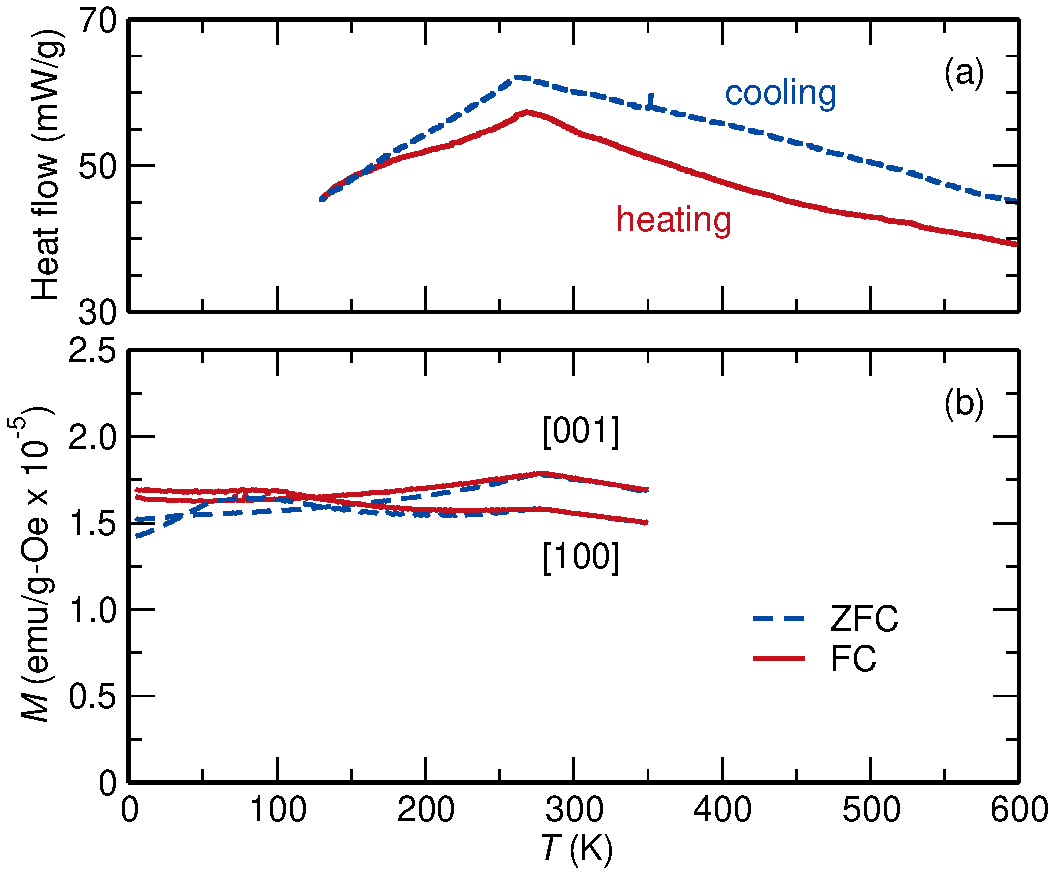
\includegraphics[width=0.6\columnwidth]{figures/ch5/dsc-mpms_norm_cropped.pdf}
\caption{
DSC data (a) show a clear kink in the heat flow at $T_N \approx 270$ K, indicating a discontinuous change in heat capacity of the sample. Data on heating are reflected about the $x$-axis. The same transition appears in magnetic susceptibility measurements (b) of an aligned single crystal, with the field axis along the [001] and [100] directions.
} 
\label{fig:dsc-mpms}
\end{figure}

The magnetic ordering was probed first by variable-temperature neutron powder diffraction
on the WAND$^2$ instrument, which showed changes in peak intensities across this boundary, but no new peaks, indicating likely $k = 0$ ordering.
A full triple-axis data collection was performed on the HB-3A beamline at 4~K.
The magnetic and nuclear structures were refined together in the $P\overline{6}^\prime$ magnetic space group. 
The intensity of the (020) peak can serve as an order parameter, and its temperature dependence is shown in Fig.\ \ref{fig:hb3a}(a).
The (020) peak is an allowed nuclear reflection, so the intensity does not go to zero above $T_N$.
The three inequivalent Mn sites are constrained to have equal magnetic moments, which are refined to 3.02(8) $\mu_B$/atom.
No improvement in the fit was observed when the moments were allowed to freely vary.
The observed and calculated structure factors $F_{hkl}^2$ are plotted in Fig.\ \ref{fig:hb3a}(b).
The magnetic structure is shown in Fig.\ \ref{fig:unitcell}(b). 
No local Mn moment was stably refined on the Cu-majority sites, and Cu itself does not host local moments in arsenides \cite{pauwels_electrical_1973,sampathkumaran_enhanced_2003,sengupta_magnetic_2005}.
It is possible that some local Mn moments exist on the minority Cu sites, but they do not appear to be ordered.
{\color{black}The 120$^\circ$ spin structure differs from Mn$_3$Sn. In Mn$_3$Sn, the spin triangles are connected by their corners. We also do not observe the ``inverse triangle'' orthorhombic configuration seen in Mn$_3$Sn \cite{Brown_1990}. There are three different types of 120$^\circ$ spin structures observed in our compound, although the spin directions in the $ab$ plane could not be uniquely determined by unpolarized neutron diffraction.}
This compound could be written as containing Cu$^+$ and Mn$^{2+}$, but like other transition-metal arsenides the local moment is reduced due to metallicity \cite{Katsuraki1966,Pytlik1985}.

\begin{figure}
\centering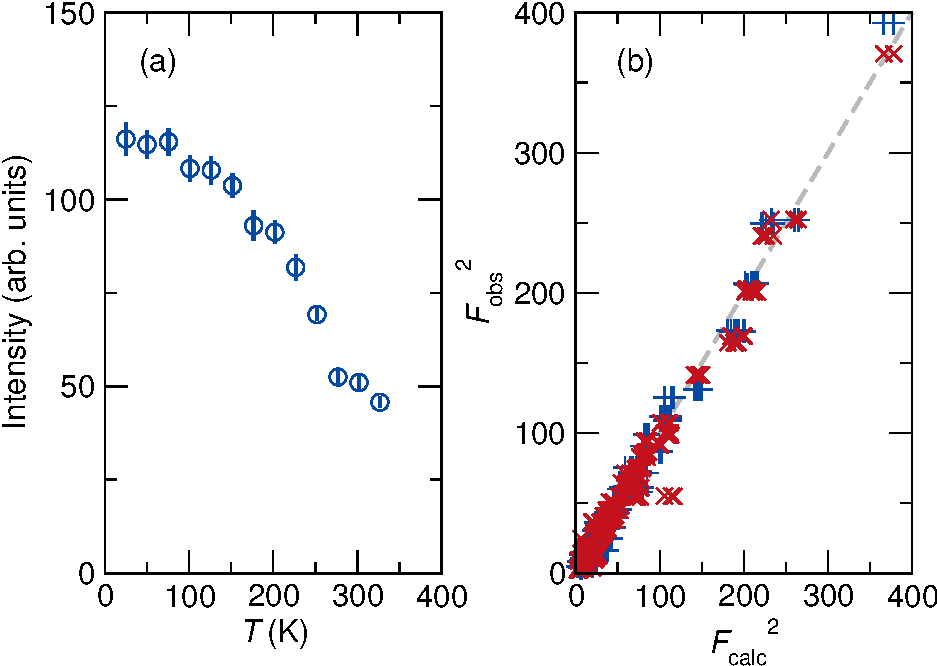
\includegraphics[width=0.6\columnwidth]{figures/ch5/hb3a_op-fobs_modified_by_manohar_cropped.pdf} \\
\caption{\label{fig:hb3a}
Measured single-crystal neutron diffraction intensity (a) of the (020) peak of Cu$_{0.82}$Mn$_{1.18}$As shows a gradual increase upon cooling past $T_N$ down to 4~K. The (020) peak is an allowed nuclear reflection and persists with constant intensity ($\sim 50$) above $T_N$. The differences between observed and refined structure factors $F_{hkl}^2$ at $T=4$~K are shown in (b). The triangular model obtained from neutron refinement are shown as ($+$) and the DFT-derived model as ($\times$).
} 
\end{figure}

\begin{figure}
\centering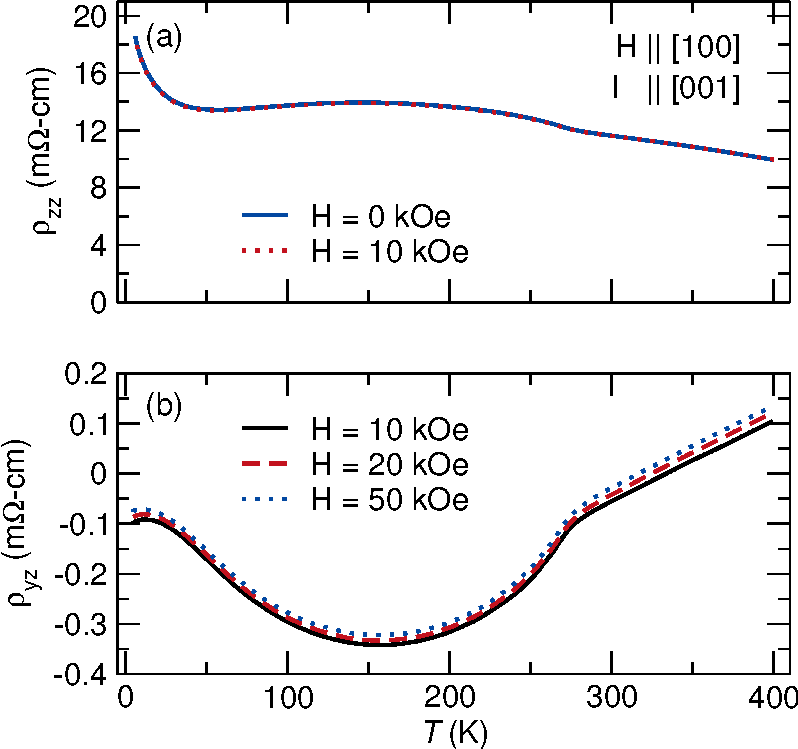
\includegraphics[width=0.6\columnwidth]{figures/ch5/resistivity_data_hall_cropped.pdf} \\
\caption{\label{fig:res-data}
(a) Resistivity of Cu$_{0.82}$Mn$_{1.18}$As with applied field $H$ along [100] and current $I$ along [001]. The resistivity is relatively flat across the temperature range, with a small kink at $T_N = 270$~K. Hall measurements of the sample with $H$ along [100] and current along [001] show a decreasing trend followed by an increase at higher temperatures. 
}
\end{figure}

Four-point probe resistivity measurements along [001] show a mostly flat, weakly undulating trend versus temperature as shown in Fig.\ \ref{fig:res-data}(a).
The broad hump between 50~K to 250~K could be attributed to competing mobilities and carrier concentrations of multiple excited states in a heavily doped semiconductor (as in P-doped Si) \cite{Chapman1963}, or variations in the dominant carrier scatterers in a disordered metal (which we discuss subsequently to be more likely, given the computed band structure).
The resistivity values are roughly 125 times higher at 5~K in \cumnas\ than Fe$_2$As and about 380 times higher than tetragonal CuMnAs, both of which are metallic \cite{Takeshita2017,Wadley2013}.
Application of a magnetic field of 10 kOe along [100]  resulted in negligible change in resistivity values, shown in Fig.\ \ref{fig:res-data}(a).
A slightly larger effect can be seen in the Hall effect measurements in Fig.\ \ref{fig:res-data}(b).
The Hall data magnifies the hump around 150~K, and crosses from negative (majority $n$-type) to positive ($p$-type) upon heating past 330~K. 
The material is $n$-type at low temperatures but as temperature is increased, more carriers are excited and the higher mobility of holes leads to compensation and switching to $p$-type conduction 330~K.
The lack of an anomaly in the total resistivity around the Hall crossover point indicates that the transport in \cumnas\ occurs via multiple bands, and is supported by the delicate (but not gapped) band structure around the Fermi energy  that we discuss subsequently. 

\subsection{First-principles simulations}

We performed first-principles density-functional theory (DFT) simulations to confirm the stability, cell geometry, and magnetic
ordering of a fully-occupied hexagonal model compound CuMnAs and off-stoichiometric Cu$_{0.89}$Mn$_{1.11}$As, with a single Mn on a Cu1 site (1 of the 9 sites substituted per cell).
We find that the relaxed atomic geometries of hexagonal CuMnAs and Cu$_{0.89}$Mn$_{1.11}$As agree with neutron scattering results within $2\,\%$.
The DFT data for the magnetic structures arrive at different lowest-energy orderings than the neutron refinement. 
The DFT-derived lowest-energy magnetic configurations
of stoichiometric CuMnAs and substituted Cu$_{0.89}$Mn$_{1.11}$As are shown in Figs.\ \ref{fig:DFT-mag}(a) and (b), respectively.
The stoichiometric result is antiferromagnetic, while 
the substituted site in Cu$_{0.89}$Mn$_{1.11}$As has a small uncompensated moment ($-0.102a - 0.010b$~\textmu$_\mathrm{B}$). 
The calculated neutron diffraction structure factors for the stoichiometric case  are compared
to the single-crystal neutron-refined values
in Fig.\ \ref{fig:hb3a}(b). 
The two fits are similar, apart from  the trio of peaks with $F_{obs}^2 \approx 100$,
which significantly degrade the fit versus the neutron result.
The neutron refinement outperforms the DFT fit with $R_{F^2} = 7.77$ and $R_{F^2w} = 17.1$ versus $R_{F^2} = 7.98$ and $R_{F^2w} =23.0$, respectively, where smaller numbers indicate a better fit. 
{\color{black}A small uncompensated moment observed in the Mn-substituted DFT model is an unavoidable artifact of the cell choice, which contains one ``extra'' Mn atom to reflect the off-stoichiometry of \cumnas.}


\begin{figure}
\centering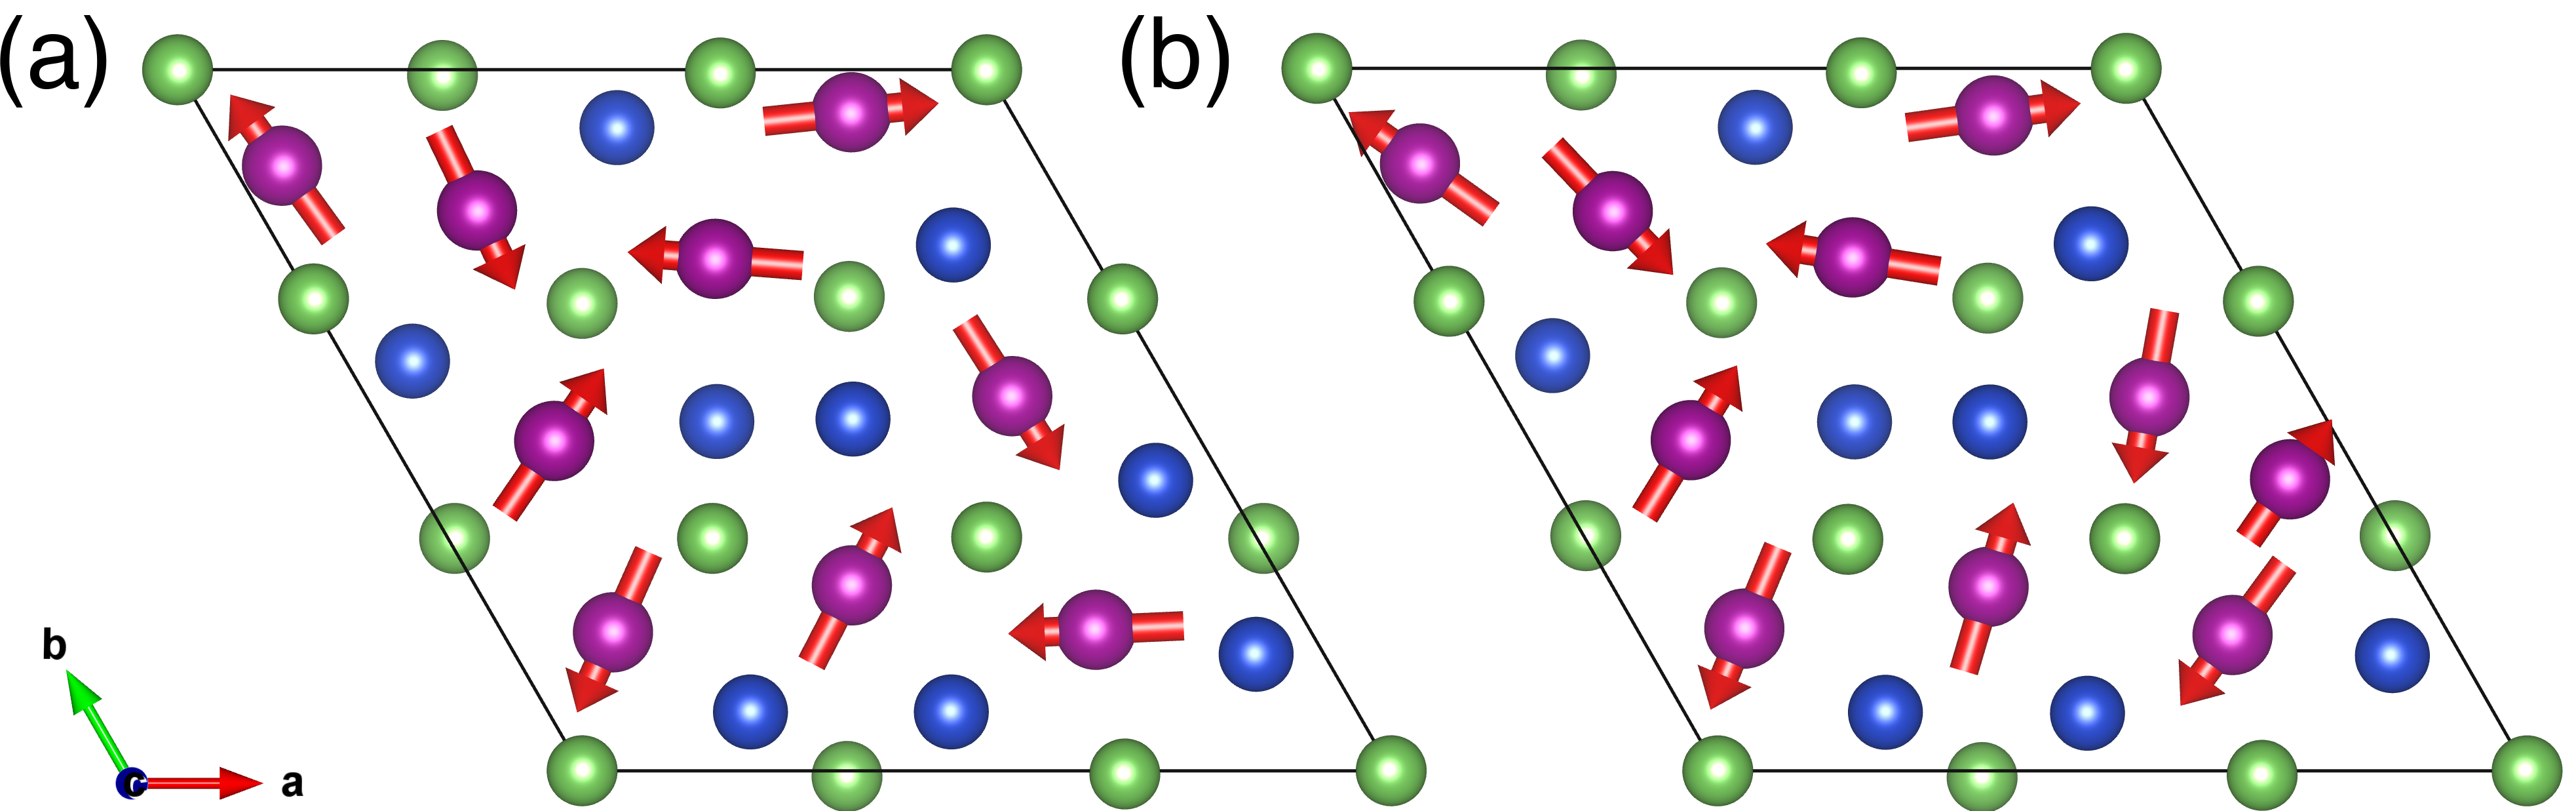
\includegraphics[width=\columnwidth]{figures/ch5/h-cumnas_1x1_dft.png} \\
\caption{\label{fig:DFT-mag}
Structure and magnetic configuration from DFT for (a) stoichiometric hexagonal CuMnAs and (b) Cu$_{0.89}$Mn$_{1.11}$As. 
Mn is shown in purple, Cu in blue, and As in green.
}
\end{figure}


Magnetic ground states in strongly-correlated $d$-electron systems are often challenging to predict using DFT,
so it is instructive to quantitatively evaluate the proximity of the neutron-refined result to the DFT energy minimum, and likewise the predicted neutron intensities of the DFT model.
To better understand the energetics of this difference between theory and experiment, we compare total energies for three different situations:
First, chemical and magnetic structures are constrained to the neutron scattering result ($E_\mathrm{fix}$ in Table \ref{tab:DFT-energy-latparam}).
Second, the ground-state magnetic structure is computed from DFT while the atomic geometries are constrained to the neutron scattering data ($E_\mathrm{mag}$ in Table \ref{tab:DFT-energy-latparam}).
Finally, these total energies are compared to the fully relaxed DFT result ($E_\mathrm{all}$ in Table \ref{tab:DFT-energy-latparam}).
These small energy changes, 15.30 and 14.93~meV/atom for CuMnAs and Cu$_{0.89}$Mn$_{1.11}$As, respectively are typical of energy differences between various magnetic structures for similar systems \cite{Alsolami2012Auth}.

\begin{table}
\caption{\label{tab:DFT-energy-latparam} 
Energy differences (meV/atom) between different constraints in DFT (see text), and lattice parameters (\AA, degree) from all-relaxed calculations of stoichiometric hexagonal CuMnAs and Cu$_{0.89}$Mn$_{1.11}$As. All phases have $\gamma = 120^\circ$.
}
\centering
\begin{tabular}{cccccc}
\hline\hline
System	 & $E_\mathrm{fix}-E_\mathrm{mag}$	 & $E_\mathrm{fix}-E_\mathrm{all}$	 & $a$	 & $b$	 & $c$ \\
\hline
CuMnAs	 & 9.92	 & 15.30	 & 11.050	 & 11.050	 & 3.802\\
Cu$_{0.89}$Mn$_{1.11}$As	 & 6.45	 & 14.93	 & 11.053	 & 11.043	 & 3.776\\
\hline \hline
\end{tabular}
~\\
\end{table}

\begin{figure}
\centering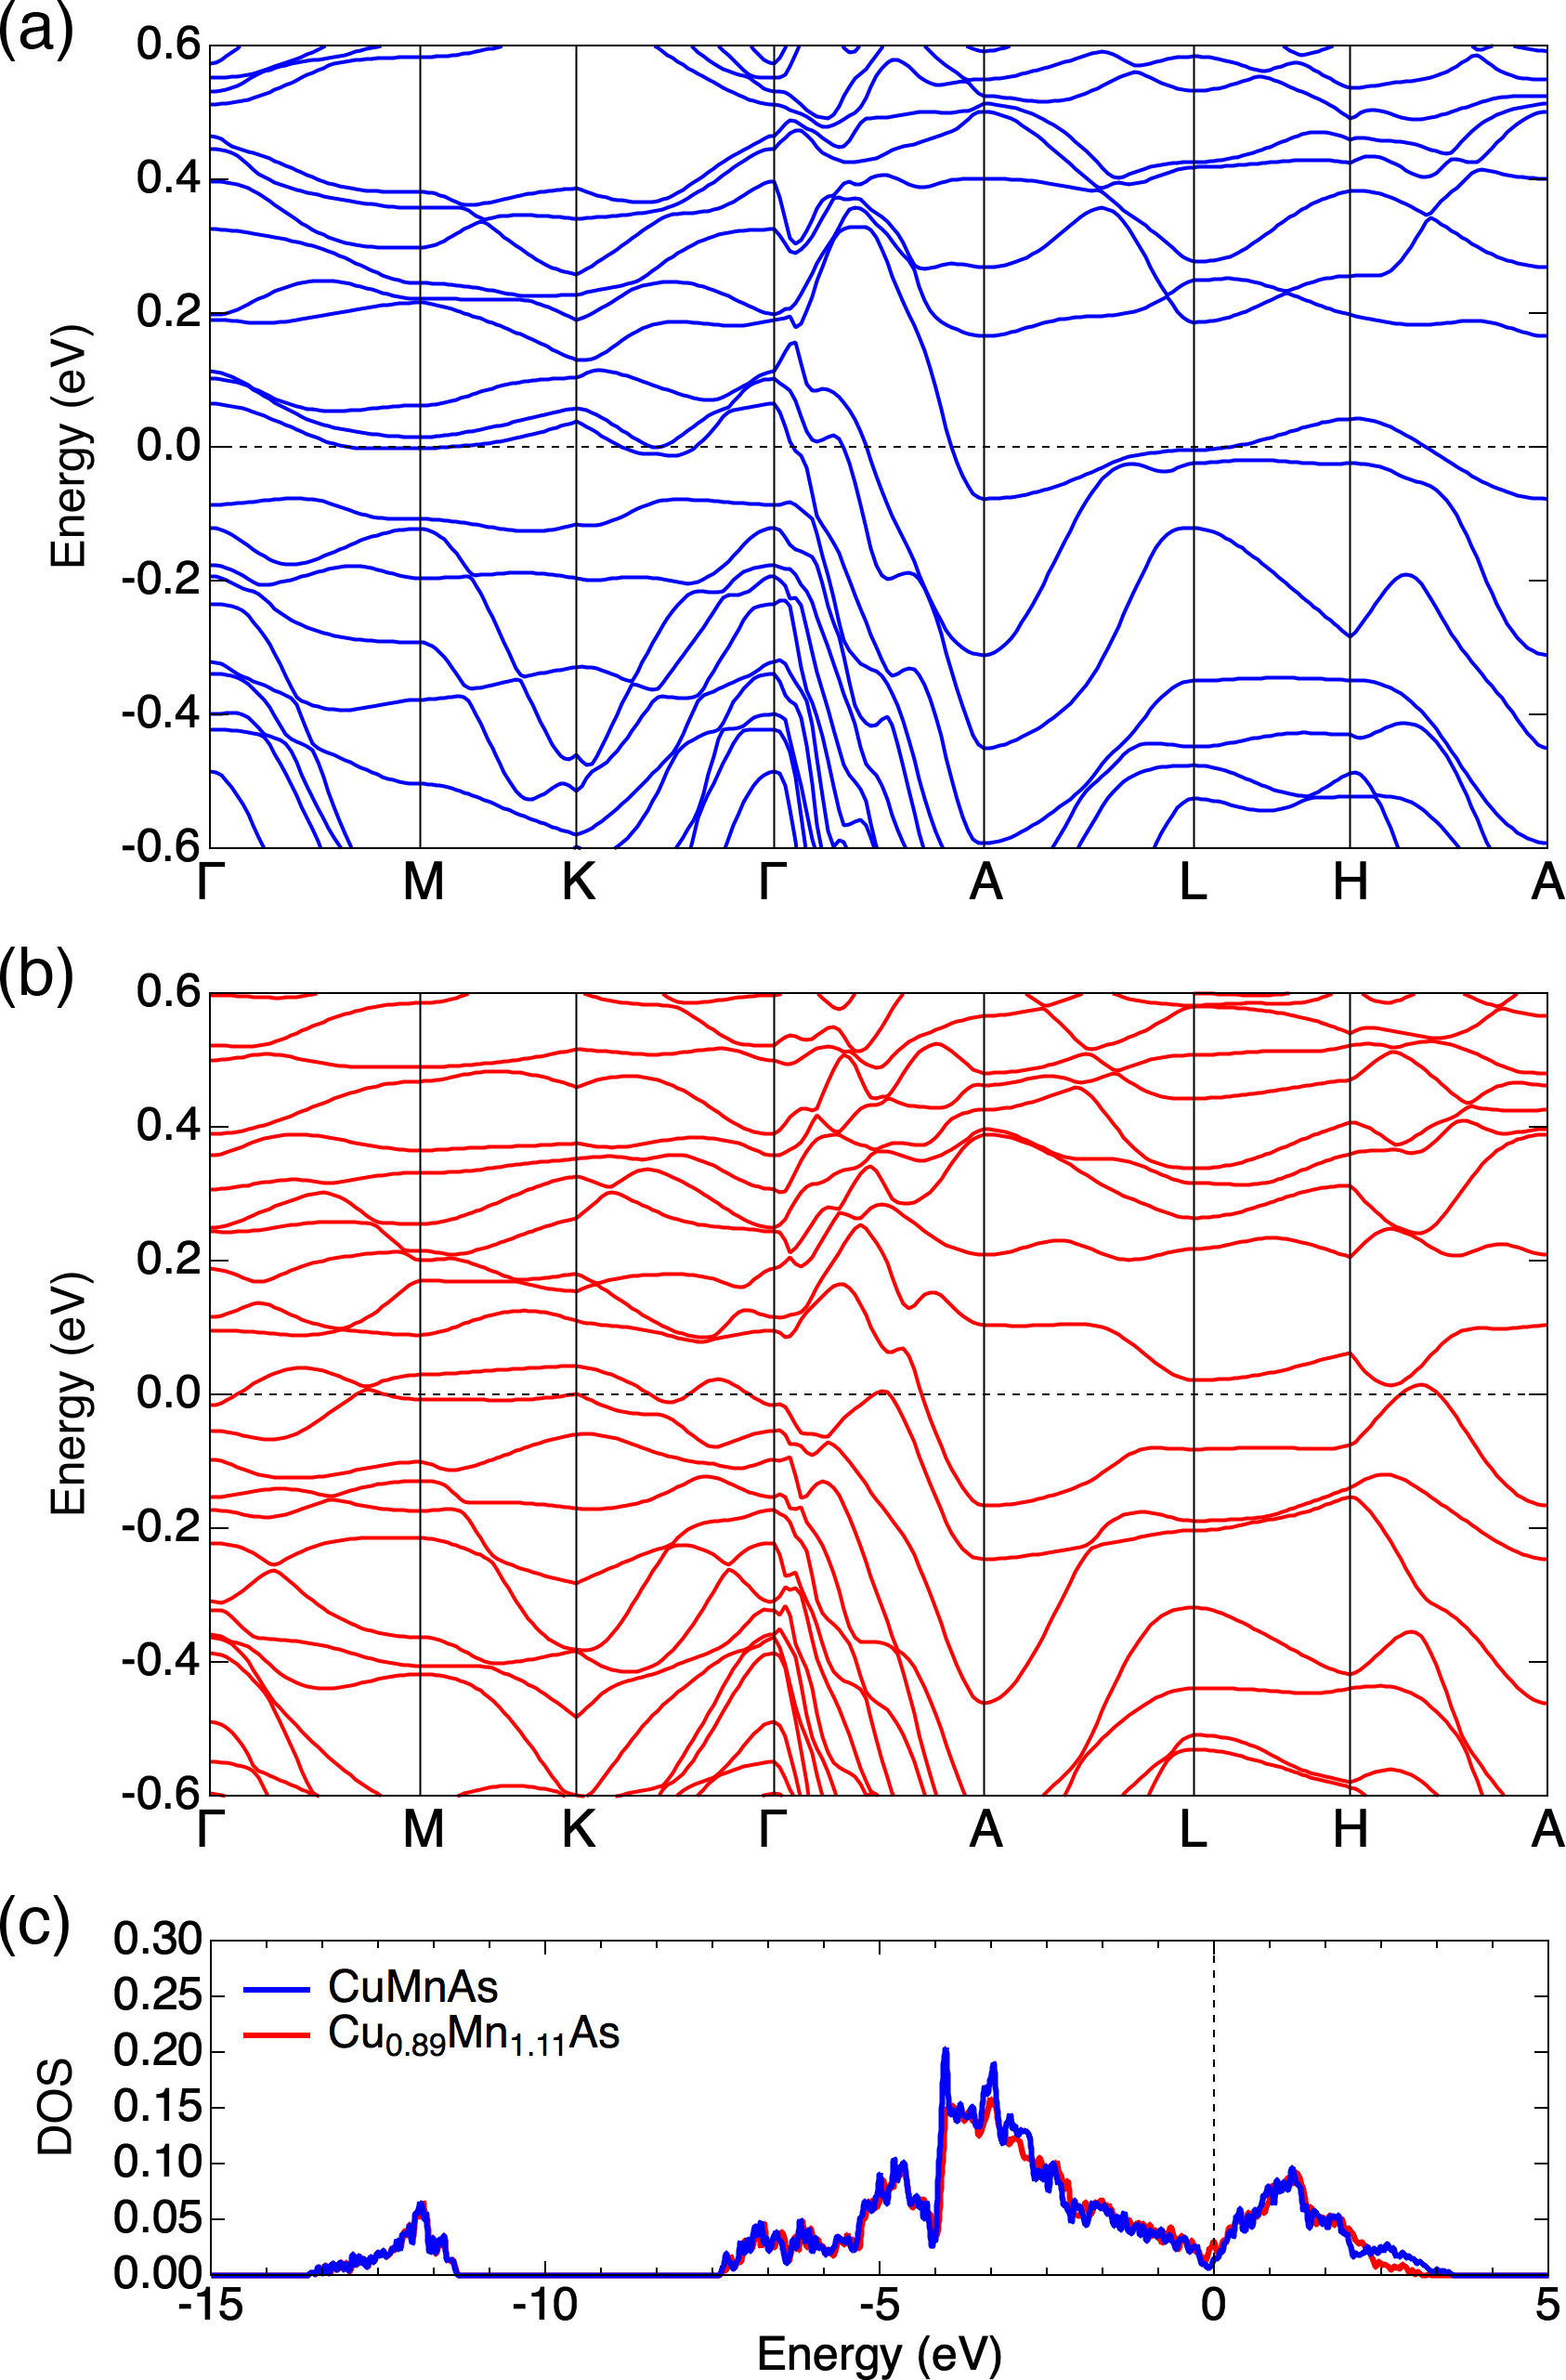
\includegraphics[width=0.7\columnwidth]{figures/ch5/h-cumnas-dft-band.png} \\
\caption{\label{fig:DFT-band}
Electronic band structure of (a) stoichiometric hexagonal CuMnAs (blue) and (b) Cu$_{0.89}$Mn$_{1.11}$As (red). Both densities of states (DOS, in units of states per \AA$^3$ and per eV per spin), computed using DFT, are shown in (c).
The highest-occupied energies are set as $E=0$ eV.
}
\end{figure}

The electronic band structure and density of states of stoichiometric hexagonal CuMnAs and Cu$_{0.89}$Mn$_{1.11}$As in Fig.\ \ref{fig:DFT-band} show that both hexagonal models are metallic.
Both electronic structures exhibit very small densities of states near the Fermi energy, similar to that described by DFT for tetragonal CuMnAs \cite{Maca2017}.
Tetragonal CuMnAs shows obvious metallic resistivity ($d\rho/dT > 0$) \cite{Wadley2013}.
The CuMnAs compounds are clearly on the cusp of semiconducting/metallic behavior, and share similarities to Fe$_2$As, which has a much greater density of states at the Fermi level and does show $d\rho/dt > 0$, but the reported values of resistivity values are much higher than that of tetragonal CuMnAs \cite{Yang2019,Takeshita2017}.


Our DFT calculations suggest that Cu$_{0.89}$Mn$_{1.11}$As is metallic. However, transport measurements indicate that the resistivity is high, and $d\rho/dT < 0$ for most $T$. 
The negative slope that is observed at low and high temperatures is not exponential as is expected in highly-doped semiconductors \cite{Chapman1963}.
The seeming discrepancy between resistivity and the computed band structure can be resolved by considering the high amount of substitutional disorder in these compounds.
Metals often exhibit $d\rho/dT < 0$ behavior when a large amount of configurational disorder is present \cite{Elk1979}, and the negative temperature dependence is in fact correlated with high absolute values of resistivity \cite{Mooij1973}.
In our material, carriers must scatter due to pervasive disorder due to Mn site mixing, while magnon scattering may also contribute strongly, but the overall resistivity is hardly affected upon cooling past $T_N$.

\section{Conclusions}

We report the crystal structure of a non-centrosymmetric $P\overline{6}^\prime$ phase in the Cu--Mn--As system, with a new structure type. This compound can be made phase-pure in single crystal form. Triangular antiferromagnetic ordering appears upon cooling below 270~K and is markedly distinct from the orthorhombic and tetragonal CuMnAs phases, both of which are stabilized by different Cu/Mn content and are centrosymmetric in their paramagnetic states. DFT calculations confirm the stability of the magnetic structure refined by single-crystal neutron diffraction. The triangular AF ordering is in-plane and does not break degeneracy of the $a$ and $b$ axes.  Like other copper manganese arsenides, hexagonal \cumnas\ is on the cusp of semiconducting/metallic behavior and further investigation of the carrier scattering mechanisms in this class of materials is warranted.


\section{Acknowledgments}

This work is supported by the National Science Foundation (NSF) under Grant No.\ DMR-1720633.
Characterization was carried out in part in the Materials Research Laboratory Central Research Facilities, University of Illinois. Use of the Advanced Photon Source at Argonne National Laboratory was supported by the U.S.\ Department of Energy, Office of Science, Office of Basic Energy Sciences, under Contract No.\ DE-AC02-06CH11357. Neutron scattering was performed at the High Flux Isotope Reactor, a Department of Energy Office of Science User Facility operated by the Oak Ridge National Laboratory.
This work made use of the Illinois Campus Cluster, a computing resource that is operated by the Illinois Campus Cluster Program (ICCP) in conjunction with the National Center for Supercomputing Applications (NCSA) and which is supported by funds from the University of Illinois at Urbana-Champaign.
We thank Junseok Oh for assistance in making contacts for resistivity measurements.

%##################chapter 6
\chapter{Two-step magnetic ordering into a canted state in ferrimagnetic monoclinic Mn$_3$As$_2$}

%\section{Copyrights and author contributions}

\hfill \break

\href{https://arxiv.org/abs/2008.01776}{Reprinted with permission from Manohar H Karigerasi, Bao H. Lam, Maxim Avdeev and Daniel P. Shoemaker, Journal of Solid State Chemistry, (2020). Copyright 2020 by the Elsevier.} In this work, I carried out SQUID and DSC measurements. I also carried out the magnetic structure refinement from NPD data and wrote the paper with help from coauthors. Bao Lam synthesized the samples and took images from SEM.


\section{Abstract}

We report the magnetic structure of monoclinic Mn$_3$As$_2$ at 3~K and 250~K using neutron powder diffraction measurements. From magnetometry data, the Curie temperature of Mn$_3$As$_2$ was confirmed to be around 270~K. Calorimetry analysis showed the presence of another transition at 225~K. At 270~K, Mn$_3$As$_2$ undergoes a $k = 0$ ferrimagnetic ordering in the magnetic space group $C2/m$ (\#12.58) with Mn moments pointing along $b$. Below 225~K, there is a canting of Mn moments in the $ac$ plane which produces a multi-$k$  non-collinear magnetic structure in space group $C2/c$ (\#15.85). The components of Mn moments along $b$ follow $k=0$ ordering and the components along $a$ and $c$ have $k = [0 0 \frac{1}{2}]$ propagation vector. The change in the magnetic ground state with temperature provides a deeper insight into the factors that govern magnetic ordering in Mn-As compounds.

%\textbf{Keywords} - magnetic structure refinement; neutron diffraction; metallic ferrimagnet; geometric frustration; non-collinear magnetic ordering; magnetocrystalline anisotropy




\section{Introduction} 



The Mn-As phase diagram contains a rich collection of phases with various magnetic structures \cite{Bacon1955,Yuzuri1960,Carrillo-Cabrera1983,Dietrich1990,Moller1993,Hagedorn1994,Hagedorn1995}. Most of the known compounds in this phase-space can be roughly divided into two groups. Compounds in one group are of the form Mn$_{2+n}$As$_{1+n}$ where, starting with stripes of square-planar Mn-As units running along $a$ at $n=0$, every additonal Mn-As involves adding an Mn-As octahedral unit in between the stripes.
In this series, monoclinic Mn$_3$As$_2$ and Mn$_4$As$_3$ correspond to $n=1$ and $2$, respectively. 
It also includes both phases of MnAs where $n=\infty$. The other group consists of tetragonal Mn$_2$As, both the high temperature phases of Mn$_3$As$_2$ and Mn$_5$As$_4$. The structures in this group can be built by constructing slabs from the components of NiAs and Ni$_2$In structure type \cite{Hagedorn1995}. Mn$_3$As and an orthorhombic Fe$_2$P structure type Mn$_2$As are few other compounds that exist in the phase space \cite{Jeitschko1972,Carrillo-Cabrera1983}.

MnAs orders ferromagnetically (FM) with the Mn moments pointing perpendicular to $c$ \cite{Bacon1955}. It changes from a hexagonal NiAs type to an orthorhombic MnP type upon change in temperature, pressure, magnetic field or chemical doping \cite{Glazkov2003,Ishikawa2006,Sirota1971,Pytlik1985,Schwartz1971}. 
The FM ordering of MnAs changes to a spiral or a canted antiferromagnetic (AFM) structure at low temperatures and high pressures \cite{Bacon1955,Andresen1984,Glazkov2003}. 
Mn$_2$As, on the other other hand, has an AFM ordering with N\'eel vector perpendicular to $c$ \cite{Austin1962}.
Despite the presence of many compounds in the Mn-As phase diagram, the magnetic structures have been studied only for MnAs and Mn$_2$As \cite{Bacon1955,Austin1962}.
Most known Mn-As compounds provide a metallic lustre upon cleaving \cite{Hagedorn1995,Hagedorn1994,Dietrich1990,Moller1993}.
With increasing interest in metallic antiferromagnets for spintronic applications \cite{Baltz2018,Siddiqui2020,Jungfleisch2018}, the Mn-As phase space provides an ideal collection of compounds to explore magnetism.

\begin{figure}
\centering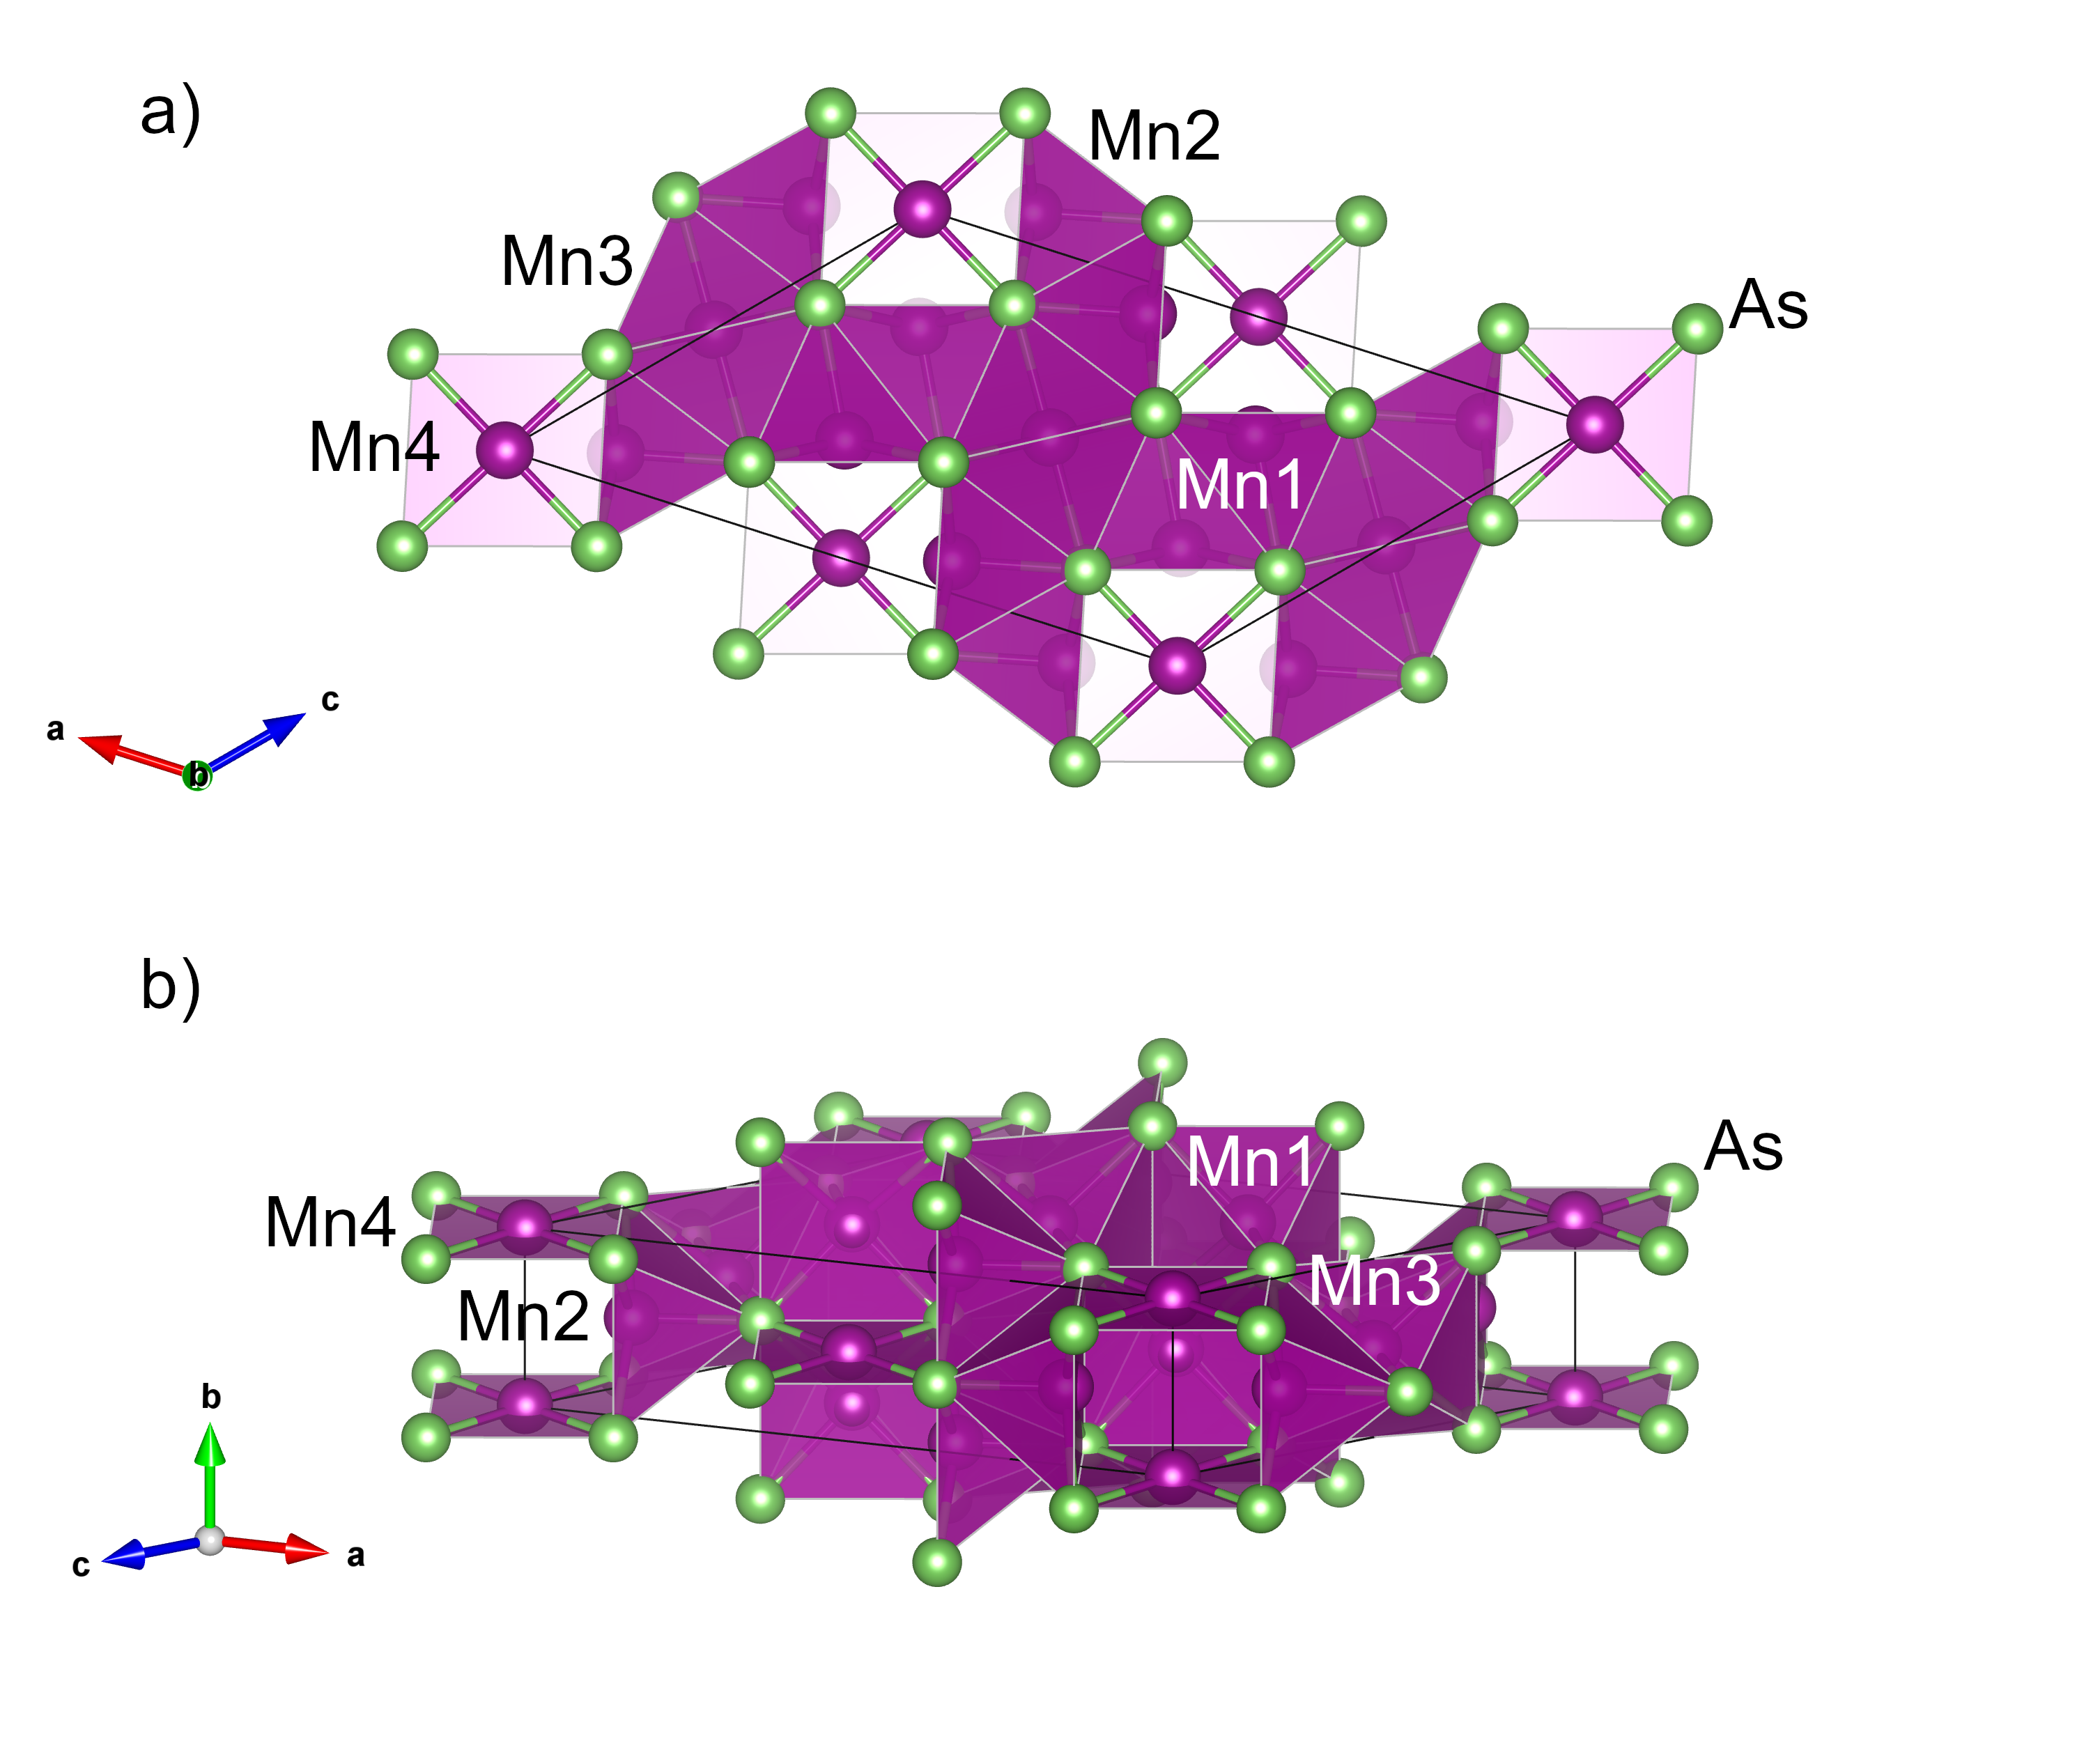
\includegraphics[width=0.8\columnwidth]{figures/ch6/monoclinic_Mn3As2_75510.png} \\
\caption{The chemical structure of Mn$_3$As$_2$ showing the four different Mn atom sites when viewed (a) along $b$ and (b) perpendicular to $b$. Mn1 and Mn2 form square pyramidal units with As, while Mn3 and Mn4 form octahedral and square planar units, respectively.
}
\label{fig:Mn3As2_crystal_structure}
\end{figure}


Mn$_3$As$_2$ is known to exist in three different structure types depending on the stoichiometry and the synthesis procedure \cite{Dietrich1990,Moller1993,Hagedorn1994}. The first variant is in monoclinic space group, which is obtained by quenching after annealing above 1023 K for 9-12 days, and contains a deficiency of Mn atoms. Transport measurements indicate that the compound is metallic \cite{Dietrich1990}. The second variant of Mn$_3$As$_2$ is in orthorhombic space group but the structure can be derived from the previous variant by changing one of the building block in Ni$_2$In structure type.
It is obtained by annealing between 873 K to 1023 K for 9-12 days and is always found to be intergrown with Mn$_5$As$_4$ crystals \cite{Moller1993}. The final variant is the structure that is stable at room temperature when Mn and As are mixed stoichiometrically. 
Single crystal needles of length 0.2~mm can also be obtained with I$_2$ as a transporting agent \cite{Hagedorn1994}.
It crystallizes in a monoclinic space group $C2/m$ with four inequivalent Mn atoms as shown in Fig. \ref{fig:Mn3As2_crystal_structure}. Mn atoms form square planar, square pyramidal and octahedral units with As and the structure is very similar to that of tetragonal V$_3$As$_2$ \cite{Hagedorn1994,Hagedorn1995}. Magnetometry measurements have indicated that the compound is ferromagnetic below 273 K and the moments saturate at 17.2~gauss per gram or 0.31~$\mu_B$ per Mn atom at low temperature \cite{Yuzuri1960}. 


In this paper, we grow room temperature stable monoclinic Mn$_3$As$_2$ using solid state synthesis and carry out magnetometry and differential scanning calorimetry (DSC) measurements to determine the transition temperatures. Using neutron powder diffraction (NPD) measurements, we identify two steps in the magnetic ordering of Mn$_3$As$_2$ and  investigate the crossover from a uniaxial to a canted magnetic  ordering.





\section{Methods}


Bulk polycrystalline Mn$_3$As$_2$ was synthesized by mixing Mn (99.98\% metals basis) and As (99.9999\% metals basis) powders in 3.1:2 ratio using a mortar and pestle inside an Ar filled glovebox. The powders were transferred into a quartz tube, vacuum sealed and heated to 873 K at 2~K/min and held for 2 hours, followed by a ramp at 1~K/min to 1273~K for 1~hour. The sample was then cooled to 1123~K at 1~K/min and held for 1~hour before it was furnace-cooled down to room temperature. The purity of the compound was checked using synchrotron powder x-ray diffraction measurements at the 11-BM beamline of the Advanced Photon Source in Argonne National Laboratory as shown in Fig. \ref{fig:11BM_data}. The final product obtained was a solid ingot that was dark gray in color with a metallic luster. Secondary electron images of the crushed Mn$_3$As$_2$ ingot were taken using JEOL JSM-6060LV low-vacuum scanning electron microscope as shown in Fig. \ref{fig:SEM_image}(a) and (b).

\begin{figure}
\centering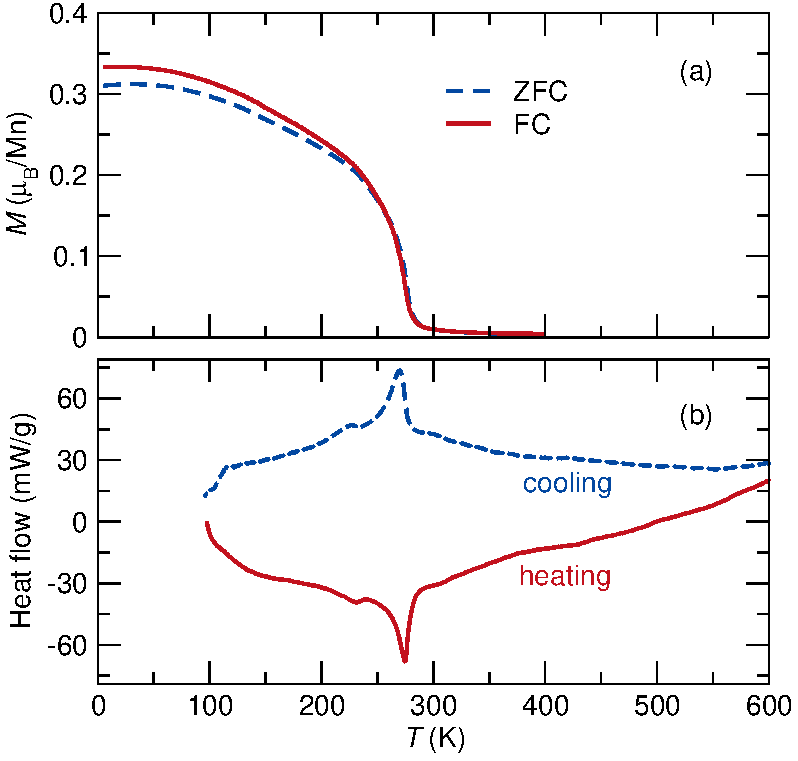
\includegraphics[width=0.75\columnwidth]{figures/ch6/FC_ZFC_DSC_Mn3As2_cropped.pdf} \\
\caption{Field cooling (FC) and zero field cooling (ZFC) of Mn$_3$As$_2$ powders in the presence of 10~kOe field clearly shows a ferromagnetic transition at around 270~K in (a). Heating and cooling curves from the DSC data in (b) show the two transitions at around 270~K and 225~K.
}
\label{fig:DSC_SQUID_measurement}
\end{figure}

\begin{figure}
\centering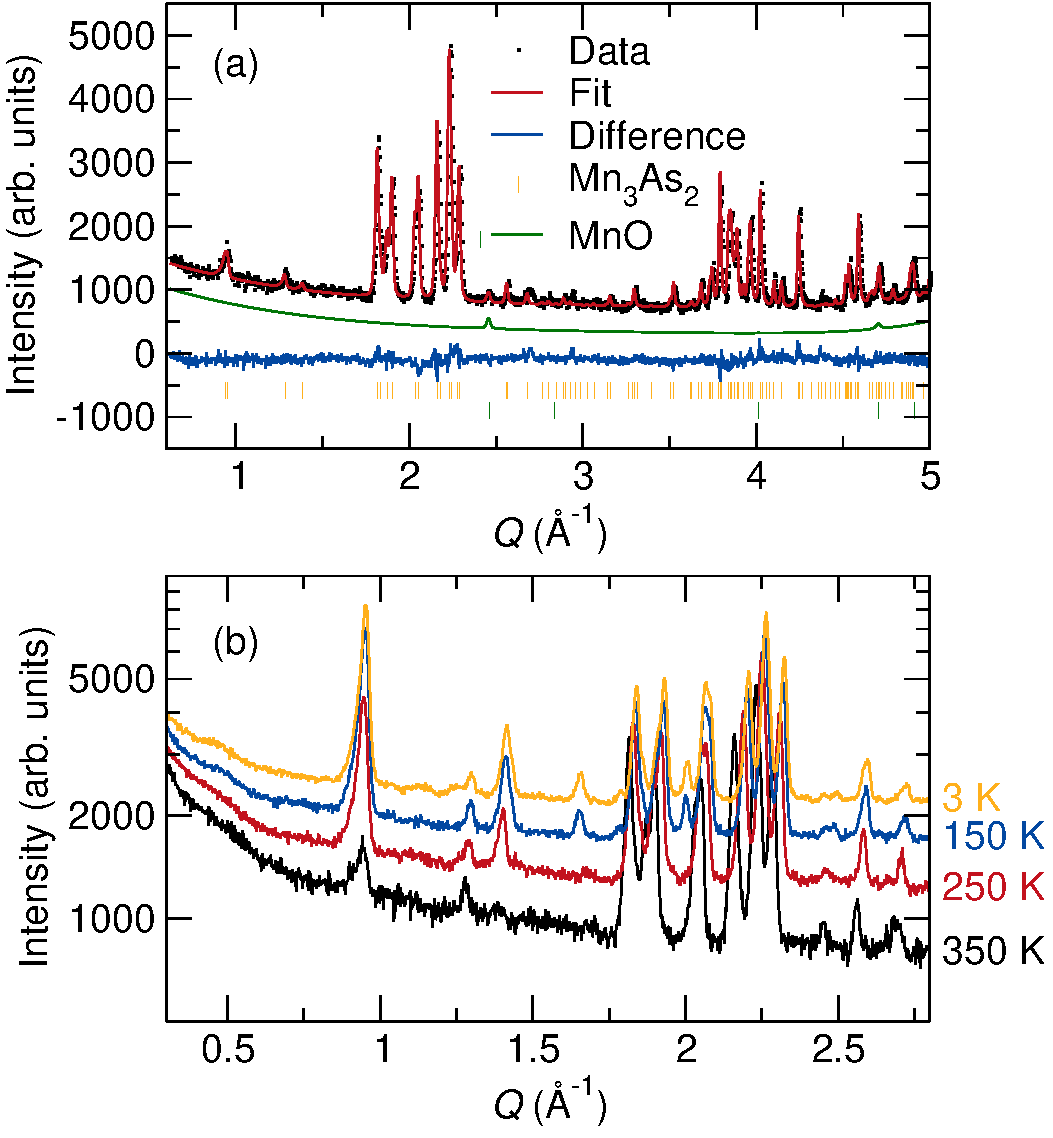
\includegraphics[width=0.75\columnwidth]{figures/ch6/350K_rietveld_diff_temp_NPD_cropped.pdf} \\
\caption{Rietveld fit to the Mn$_3$As$_2$ NPD data at 350 K is shown in (a). The contribution from the MnO impurity to the fit is also shown. The change in the NPD data due to magnetic transitions upon cooling from 350~K to 3~K is shown in (b). At $T_C = 270$~K, the intensity grows noticeably in the lowest-angle peak, while new peaks appear at the spin-canting transition around 225 K at $Q = 1.65$~\AA$^{-1}$ and 2.0~\AA$^{-1}$.
}
\label{fig:350K_data}
\end{figure}


DSC measurement was carried out on 3.6 mg of powdered sample using Al pans under N$_2$ atmosphere in a TA Instruments DSC 2500. The sample was subjected to a heat-cool-heat cycle between 93~K and 673~K at 10~K/min rate.
Magnetometry was performed on 30.6~mg of powder in a snap-shut sample holder in a Quantum Design MPMS3. The sample was cycled between 400~K and 5~K at 5~K/min in the presence of 10~kOe magnetic field for measuring field cooling (FC) and zero field cooling (ZFC) curves. NPD measurements were carried out on 1.13~g of Mn$_3$As$_2$ powder at the \textsc{ECHIDNA} high resolution powder diffractometer \cite{Avdeev2018} at the Australian Centre for Neutron Scattering. The measurements were done at 3~K, 150~K, 250~K and 350~K. Magnetic structure refinement was carried out using the \textsc{GSAS-II} software \cite{Toby:aj5212} and the \textsc{k-Subgroupsmag} program \cite{Perez-Mato2015} available at the Bilbao Crystallographic Server.



\section{Results and Discussion}


FC and ZFC curves in Fig. \ref{fig:DSC_SQUID_measurement}(a) show a clear onset of local magnetic moments near 270~K and the saturation magnetization of 0.33~$\upmu_B$/Mn for field cooling is very close to the reported value of 0.31~$\upmu_B$/Mn \cite{Yuzuri1960}. The Curie temperature was also confirmed by DSC measurements in Fig. \ref{fig:DSC_SQUID_measurement}(b). Surprisingly, another transition at around 225~K was observed in the DSC data. This transition is not obvious in the magnetometry data although there seems to be splitting of the FC and ZFC curves at around 225~K. To determine the nature of this transition, whether structural or magnetic, neutron powder diffraction was carried out on these samples at varying temperatures.

\begin{figure}
\centering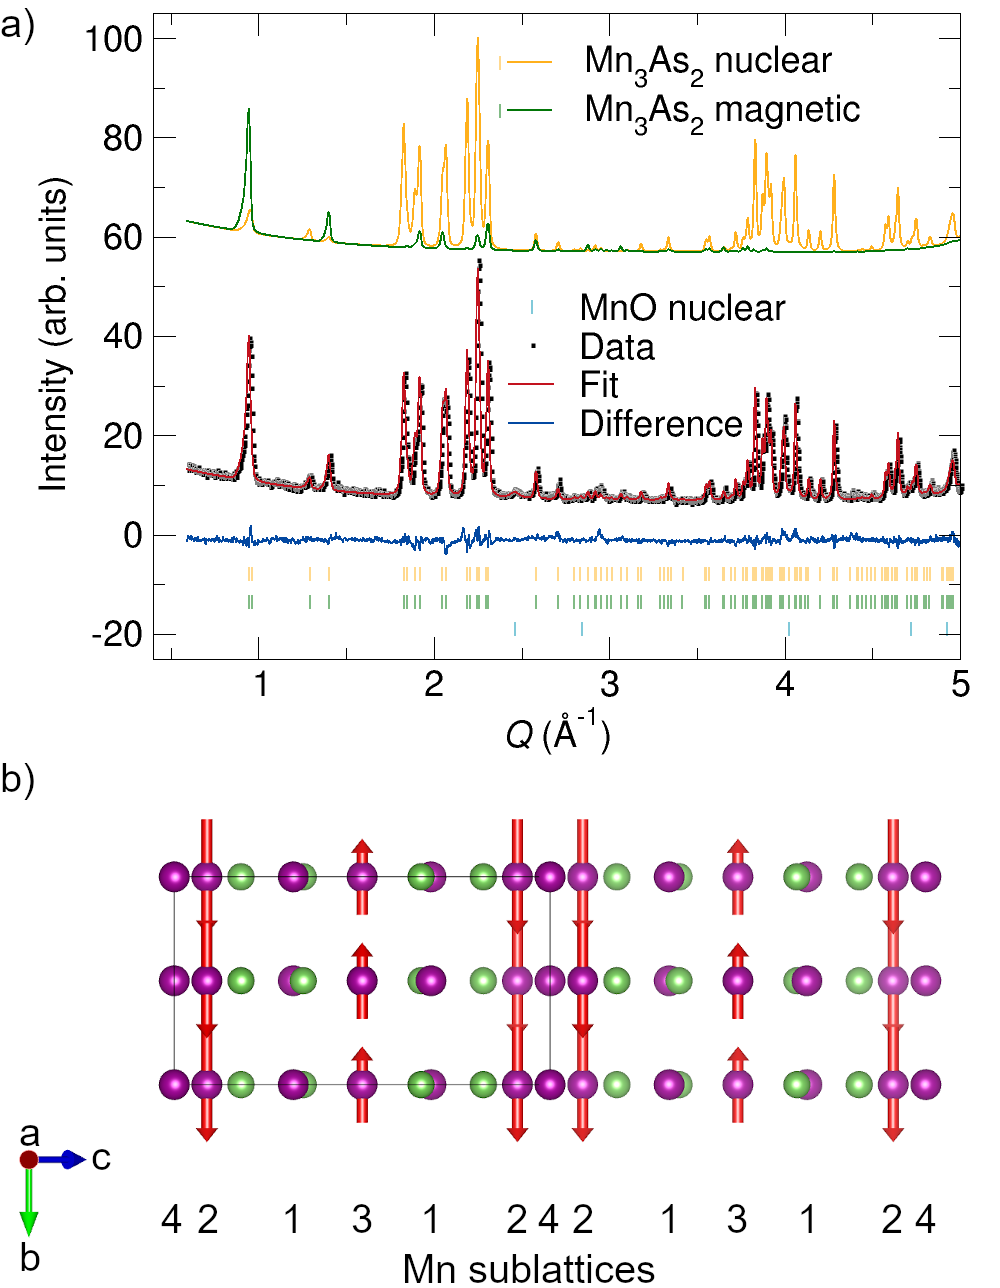
\includegraphics[width=0.75\columnwidth]{figures/ch6/250K_mag_structure.png} \\
\caption{The Rietveld fit with nuclear and magnetic contributions to the NPD data at 250~K is shown in (a). In (b), the refined magnetic structure is shown. All Mn moments point along $b$ (Mn1 and Mn4 moments are small and along -$b$ and +$b$ directions respectively) and the propagation vector is $k = 0$. 
}
\label{fig:250K_data}
\end{figure}

\begin{figure}
\centering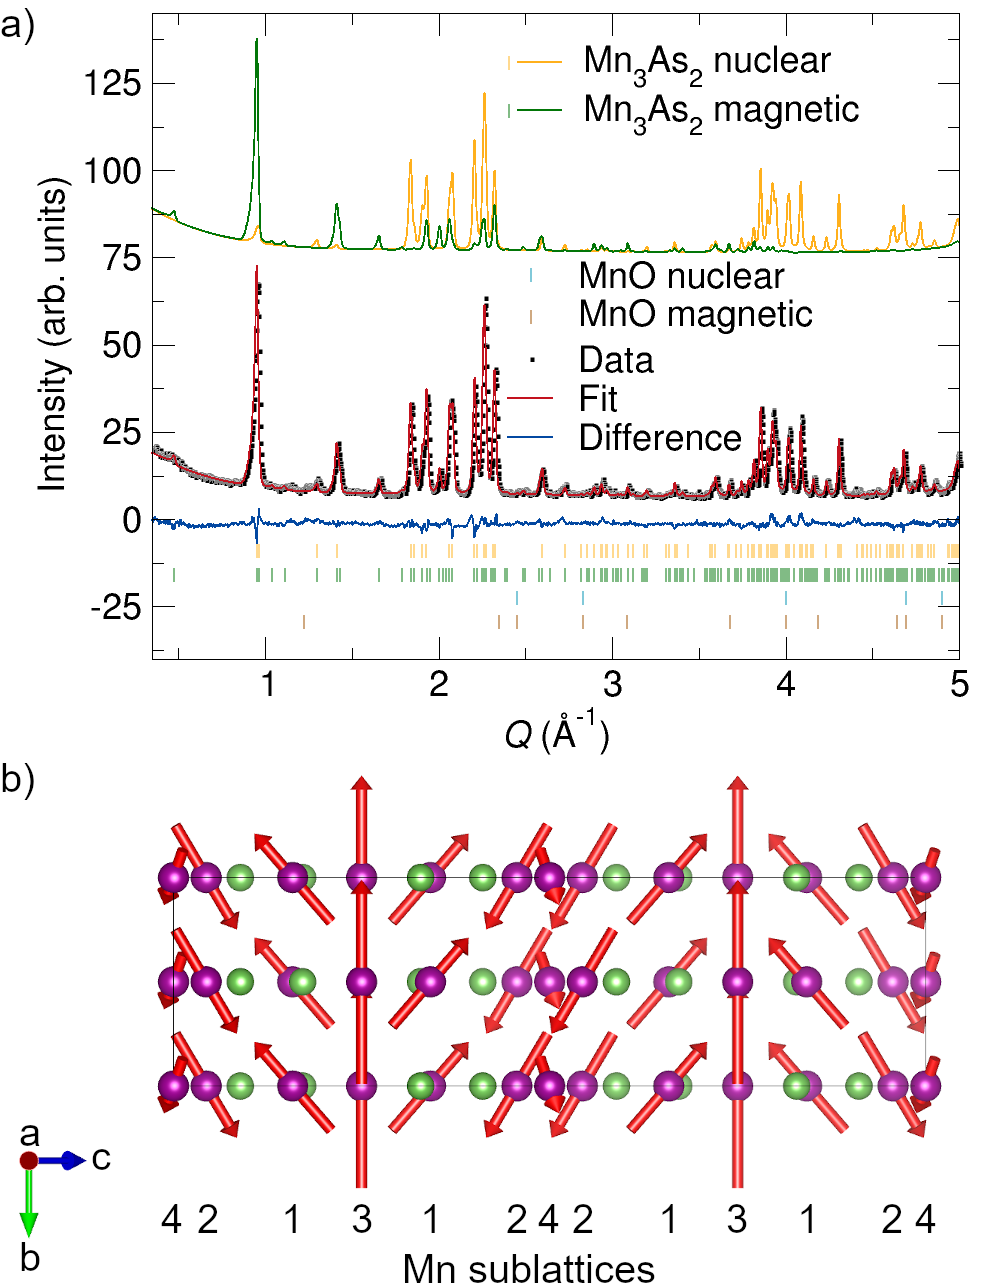
\includegraphics[width=0.75\columnwidth]{figures/ch6/3K_mag_structure.png} \\
\caption{Rietveld fit (a) to the NPD data at 3~K for the magnetic structure shown in (b). There is a canting of spins in the $a-c$ plane which results in multiple magnetic ordering vectors $k = 0$ and $k = [00\frac{1}{2}]$. The nuclear and the magnetic contribution to the fit is also shown in (a). 
}
\label{fig:3K_data}
\end{figure}


The Rietveld fit to the NPD data at 350 K in Fig. \ref{fig:350K_data}(a) confirms the paramagnetic nature of Mn$_3$As$_2$ above 270~K. About 0.6 wt\% of MnO was present as impurity and its contribution to the NPD data is shown in Fig. \ref{fig:350K_data}(a). Subsequent Rietveld fits to the NPD data at different temperatures also account for the nuclear contribution from the MnO impurity phase. Cooling from 350~K to 3~K introduces additional peaks that are magnetic in nature as seen in Fig. \ref{fig:350K_data}(b).
At 250 K, the intensities of the peaks near $Q = 0.95$~\AA$^{-1}$ and 1.4~\AA$^{-1}$ increase considerably. Since both peaks are not structurally forbidden, the magnetic unit cell remains the same as the chemical unit cell.
At 150~K, we can see new magnetic peaks near $Q = 1.65$~\AA$^{-1}$ and 2.0~\AA$^{-1}$. Fits to these patterns confirm the kink observed in the DSC data at 225~K to be a magnetic transition. The NPD patterns remain consistent upon further cooling, so we are confident the magnetic structure does not change between 150~K and 3~K. The T$_N$ of MnO is 120~K but the intensity from the magnetic peaks of MnO are too weak to be observed here. MnO magnetic peaks do not overlap with any of the Mn$_3$As$_2$ magnetic peaks and we provide markers corresponding to the MnO magnetic peaks at 3~K NPD data.



The magnetic ordering vector of Mn$_3$As$_2$ at 250~K is $k = 0$. The indices of the two magnetic peaks correspond to $(001)$ and $(20\overline{2})$ respectively. Since the magnetic peaks are of the form $(h0l)$, it is likely that the Mn moments would prefer to orient along $b$. In the $C2/m$ space group with propagation vector $k=0$, there are four possible $k$-maximal subgroups that are consistent with this propagation vector. The four subgroups correspond to different combinations of the addition of the time reversal operator to the 2-fold axis and the mirror plane. 
Of the four models, two models restrict the Mn moment orientation to the $b$ axis and the other two restrict Mn moments to lie in the $ac$ plane. 
One model from each pair results in an AFM structure and provides a poor fit to the NPD data. 
The best fit (R$_{wp}$ = 5.087\%) is unambiguously obtained for the model with $C2/m$ space group symmetry where all Mn moments point along the $b$ axis as shown in Table \ref{tab:refinement_250_K}.
The refined Mn moments for this ferrimagnetic structure are provided in Table \ref{tab:Mn_moments}. The net moment is 0.43(5)~$\upmu_B$/Mn which is close to the saturation moment of 0.33~$\upmu_B$/Mn from magnetometry. The Rietveld fit of this model to the NPD data and the magnetic structure are shown in Fig. \ref{fig:250K_data}(a) and (b), respectively. 


\begin{sidewaystable}
\caption{\label{tab:Mn_moments} 
The magnetic space groups, propagation vectors (k-vectors), magnetic irreducible representations (mag IRs) and the Mn moments in $\upmu_B$ for the magnetic structures at two different temperatures.
}
\centering
\begin{tabular}{p{1.5cm}p{2cm}p{2.2cm}p{2.6cm}p{2.15cm}p{2.15cm}p{2.15cm}p{2.15cm}}
\hline\hline
\textbf{T (K)} & \textbf{MSG} & \textbf{k-vectors} & \textbf{mag IRs} & \textbf{Mn1 (x,y,z)} & \textbf{Mn2 (x,y,z)} & \textbf{Mn3 (x,y,z)} & \textbf{Mn4 (x,y,z)}\\
\hline\hline
250 & $C2/m$ & 0 & mGM$_1^+$ & 0.00 & 0.00 & 0.00 & 0.00\\
& ($\#$12.58) & & & -0.52(9) & 2.55(9) & -1.69(14) & 0.59(6)\\
& & & & 0.00 & 0.00 & 0.00 & 0.00\\
\hline
3 & $C2/c$ & 0, $[00\frac{1}{2}]$ & mGM$_1^+$ + mA$_2^+$ & 1.24(15) & 0.87(15) & 0.00 & -0.91(16)\\
& ($\#$15.85) & & & -1.94(8) & 2.28(7) & -4.48(13) & 1.21(6)\\
& & & & 2.27(11) & 1.82(10) & 0.00 & -0.56(11)\\
\hline\hline
\end{tabular}
~\\
\end{sidewaystable}

All magnetic peak locations in the NPD data at 3~K and 150~K can be indexed using a propagation vector of $k = [00\frac{1}{2}]$. However, none of the magnetic structures from the subgroups consistent with this propagation vector provide a good fit to data and all magnetic structures obtained are AFM, inconsistent with magnetometry. Refining the 250~K model to the low-temperature NPD data provides a good fit to the two previously-existing magnetic peaks but none of the additional peaks can be fit using this model. For these reasons, it is clear that below 225~K, Mn$_3$As$_2$ contains two propagation vectors, $k = 0$ and $k = [00\frac{1}{2}]$. 


With $C2/m$ as the parent space group and using both propagation vectors, there are 16 possible $k$-maximal subgroups. 
Since the magnetic irreducible representations (irreps) of the 4 $k$-maximal subgroups in each propagation vector are one-dimensional, there is a one to one correspondence between the irreps and the space groups. The 16 $k$-maximal subgroups are obtained by mixing the 4 irreps from one propagation vector with the 4 irreps from the other propagation vector.
Expecting that the low-temperature magnetic ordering is similar to the one at 250~K, we can choose the 4 subgroups that contain the same irrep as the 250~K structure. 
This leaves us with 2 magnetic structures each in $C2/c$ and $C2/m$ space groups. The $C2/m$  magnetic structures contain all Mn moments pointing along $b$, but none of the fits provide required intensity at the $Q = 2.0$~\AA$^{-1}$ magnetic peak. As shown in Table \ref{tab:refinement_3_K}, out of the two magnetic structures with $C2/c$ space group, the best fit (R$_{wp}$ = 5.852\%) was obtained for the structure where the Mn3 moment was constrained by symmetry to be along $b$ and all other moments were allowed to tilt away from $b$. Moving to lower symmetry does not justify the additional 7 or 8 variables in the refinement. The magnitudes of the refined Mn moments are given in the Table \ref{tab:Mn_moments}. The magnetic structure along with the refined fit to the NPD data at 3~K is given in Fig. \ref{fig:3K_data}. The mcif files for both the magnetic structures are attached in the Supplementary section.

\begin{figure}
\centering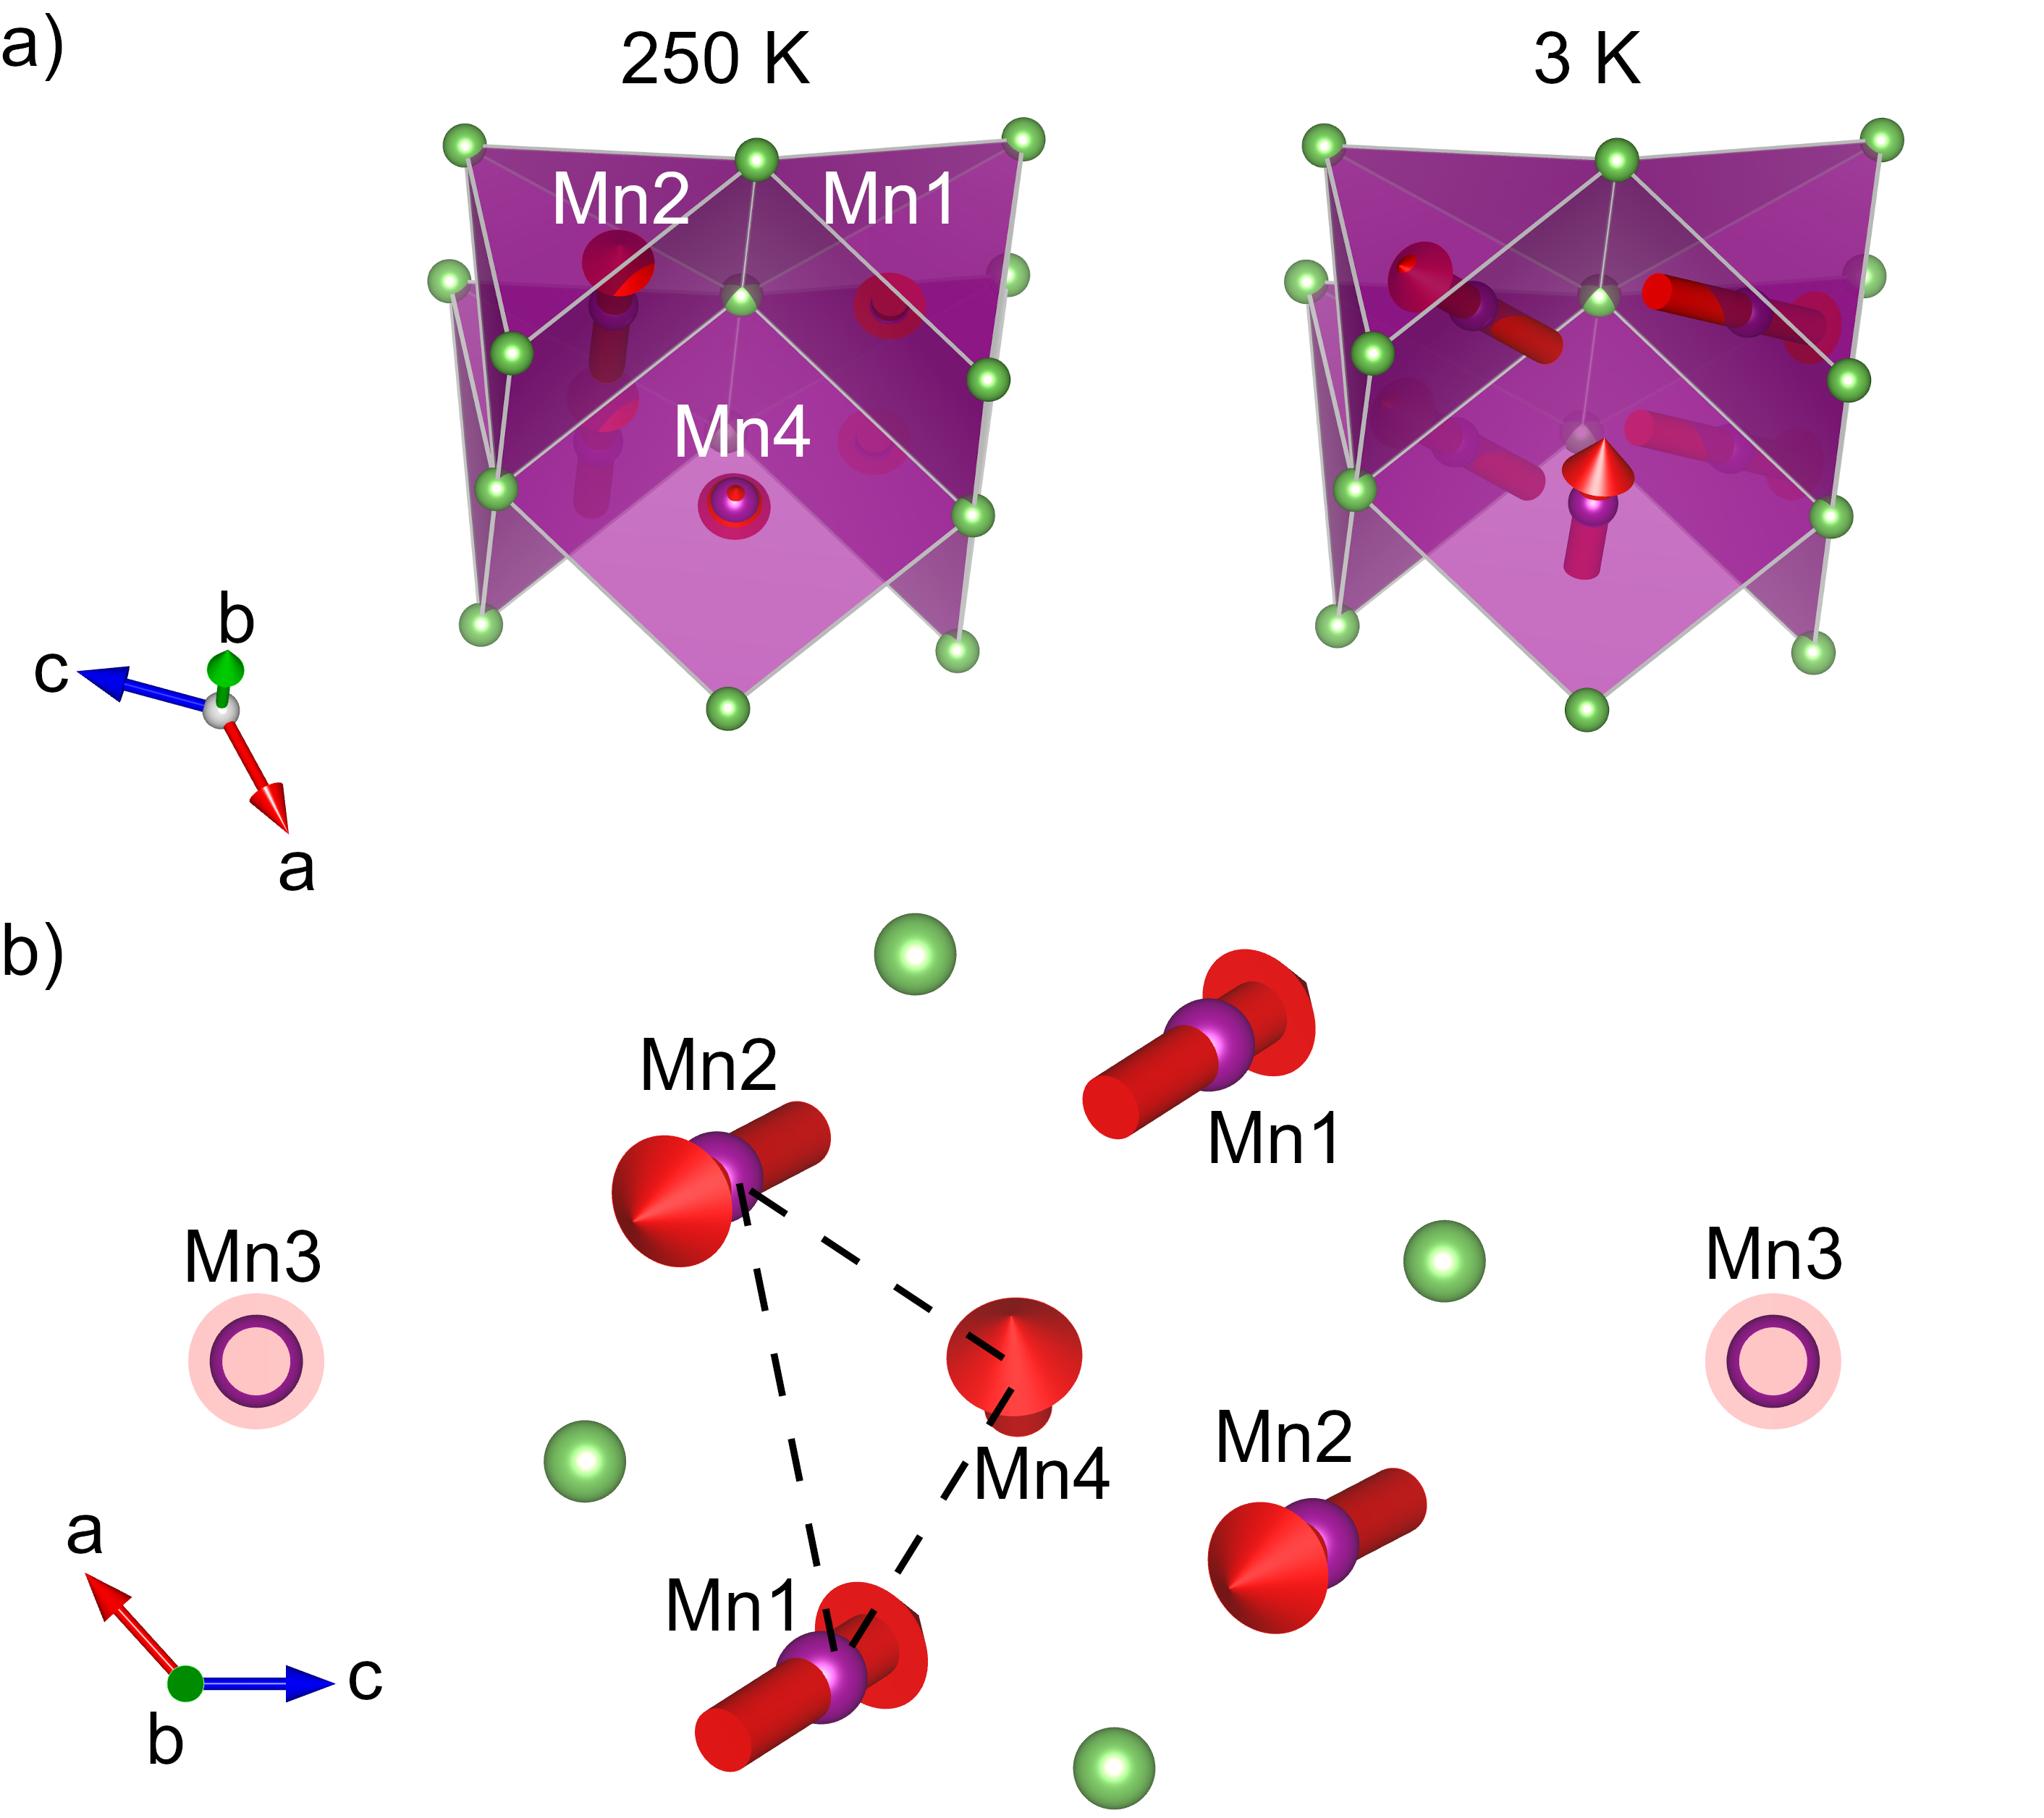
\includegraphics[width=0.75\columnwidth]{figures/ch6/spin_canting_dps.png} \\
\caption{At 250~K, large moments are present within the basal plane of square pyramidal units of Mn1 and Mn2 atoms (left, (a)). Upon decrease in temperature, there is ordering of Mn4 moments (right, (a)) which induces canting in Mn1 and Mn2 moments as well. (b) shows the geometric frustration due to antiferromagnetic interactions between Mn1, Mn2 and Mn4 moments.
}
\label{fig:spin_canting}
\end{figure}



There are 80 entries having two propagation vectors in the MAGNDATA database \cite{Gallego2016_1,Gallego2016_2}, which is about 7\% of all structures reported in the database. Hence, although less common, it is not rare to find compounds with multi-k structures. However, more than half of the compounds have either a collinear spin arrangement or contain a secondary $k = 0$ ordering to account for the presence of homogeneous magnetic moments \cite{Klepov2019,Mekata1978}. Of the remaining compounds, a common theme is to have multiple propagation vectors (k-vectors) act on different sublattices at different temperatures \cite{Zhang2019,Yi2015,Jin2013} or contain 2 k-vectors belonging to the k-star of the active irrep \cite{Skanthakumar1991}. There are less than ten compounds in the database where multiple irreps from different k-vectors act on the same magnetic sites at different temperatures like in our case.


A quick look at the magnetic transitions in this compound might lead one to compare with the ordering in triangular antiferromagnets with a small uniaxial anisotropy such as CsNiCl$_3$ and CsNiBr$_3$ \cite{Collins1997}. Upon cooling from the paramagnetic state in triangular antiferromagnets, the spins are first ordered collinear along the easy axis and then undergo another transition to form a non-collinear frustrated triangular arrangement with one of the three spins pointing along the easy axis. However, the frustration in Mn$_3$As$_2$ is along the $a-c$ plane as shown in Fig. \ref{fig:spin_canting}(b) and not $a-b$ or $b-c$ plane as would be expected if it were a triangular antiferromagnet. Hence, the anisotropy in Mn$_3$As$_2$ is not simply uniaxial below 225~K. There is some driving force that favors frustration in the $a-c$ plane which, according to our hypothesis, arises from the anisotropy of Mn4 moments.
In metallic antiferromagnets such as Mn$_2$As, tetragonal and orthorhombic CuMnAs \cite{Austin1962,MacA2012,Wadley2013}, all Mn moments in square pyramidal units with As are oriented within the basal plane rather than along the 4-fold symmetric axis.
Hexagonal Cu$_{0.82}$Mn$_{1.18}$As is a frustrated system and hence, the Mn moments slightly deviate from this arrangement \cite{Karigerasi2019}.
There are no magnetic structures reported in the MAGNDATA database \cite{Gallego2016_1,Gallego2016_2} where Mn forms square planar units with As, as in Mn4 atoms in Mn$_3$As$_2$. The canting of spins in Mn$_3$As$_2$ can be explained if we assume that the Mn spins, when bonded with As in these square planar units, prefer to orient in-plane.



In Mn$_3$As$_2$ at high temperatures, the molecular fields from other Mn moments induces a net moment in square-planar Mn4 along $b$, as shown in Fig. \ref{fig:spin_canting}(a). The value is small (0.59~$\upmu_B$) at 250~K from Table \ref{tab:Mn_moments}. Such behavior has also been observed in other arsenides such as Cr$_2$As where the Cr2 sublattice orders first at 393~K and induces a weak moment in the Cr1 atoms. The Cr1 moments order at a much lower temperature at around 175~K \cite{Ishimoto1995}.
At 225~K, the magnetocrystalline anisotropy of Mn4 moments becomes significant compared to the thermal energy and the moments acquire components along $a$ and $c$. Through exchange interactions with Mn1 and Mn2 moments, there is a canting of the Mn1 and Mn2 moments as well away from $b$, as shown in Fig. \ref{fig:spin_canting}(a). The non-collinear arrangement of Mn spins is further enhanced through geometric frustration in the $a-c$ plane due to competing AFM interactions between Mn1, Mn2 and Mn4 moments sitting on a distorted equilateral triangle as shown in Fig. \ref{fig:spin_canting}(b). There are not enough data points in the linear paramagnetic regime of the inverse susceptibility curve to provide a Curie-Weiss fit as shown in Fig. \ref{fig:inverse_susceptibility}.
The coordination environments of Mn atoms in Mn$_3$As$_2$ have point symmetry $m$ and $2/m$, not the highest allowed by their immediate coordination environments (which are distorted), but the single-site anisotropies still seem to broadly obey the trend of basal-plane preference in square pyramids and square planes.  This consistency provides opportunity to design magnetic structures by choosing specific magnetic motifs, even in low-symmetry compounds. 

The symmetry-breaking spin canting in Mn$_3$As$_2$ may at first glance seem surprising, given the nominal Mn$^{2+}$ and $3d^5$ electron configuration, but magnetocrystalline anisotropy in Mn-containing arsenides is  quite complex. Even within a set of compounds with common cation oxidation state and anion character and coordination, the spin-orbit coupling of excited and occupied states plays a major role, and typically requires computational investigation \cite{Duboc2016}.
Among compounds with two propagation vectors, inelastic neutron scattering of SrHo$_2$O$_4$ powders was used to reveal that single-ion anisotropies of the Ho sites could explain the zig-zag chain ordering in the compound \cite{Fennell2014}. TbOOH is another 2-k non-collinear compound that also has a $k = 0$ ordering. From dipolar energy calculations, the non-collinear arrangement was attributed to the crystal field anisotropy of the Tb$^{3+}$ ions which results in anisotropic exchange interactions between Tb ions \cite{Christensen1974}.
The specific energy scales that are relevant in Mn$_3$As$_2$ require further computational work and a broader set of materials to investigate. 

\section{Conclusion}

The magnetic structure of monoclinic Mn$_3$As$_2$ was identified using neutron powder diffraction experiments. From SQUID magnetometry measurements, it was identified that the material is a weak ferromagnet below 270~K. DSC data indicated another transition at around 225~K. From NPD data at 250~K, it was found that Mn$_3$As$_2$ is a ferrimagnet with all Mn moments ordering along $b$. Between 225~K to 270~K, the compound has a $k = 0$ magnetic ordering. Below 225~K, there is a canting of spins in the $a-c$ plane and it has a multi-k ordering structure with an additional $k = [00\frac{1}{2}]$ propagation vector. Here, the component of Mn moments along $b$ follow $k = 0$ ordering and the moments are uncompensated. The component of Mn moments along $a$ and $c$ follow $k = [00\frac{1}{2}]$ ordering. This behavior can be explained by considering that Mn moments align in the plane of the square planar or square pyramidal Mn-As units. Mn4 atoms are bonded to As in square-planar units within the $a-c$ plane. The lower temperature transition simply corresponds to the ordering temperature of the Mn4 sublattice.  Below 225~K, Mn4 moments cause spin canting in Mn1 and Mn2 moments through exchange interactions. Geometric frustration between Mn1, Mn2 and Mn4 moments cause significant deviation from the collinear arrangement of spins.

\section{Acknowledgments}
This work was undertaken as part of the Illinois Materials Research Science and Engineering Center, supported by the National Science Foundation MRSEC program under NSF Award No. DMR-1720633. 
The characterization was carried out in part in the Materials Research Laboratory Central Research Facilities, University of Illinois.
Use of the Advanced Photon Source at Argonne National Laboratory was supported by the U.~S. Department of Energy, Office of Science, Office of Basic Energy Sciences, under Contract No. DE-AC02-06CH11357.

\section{Supplementary}


\begin{figure}[h]
\centering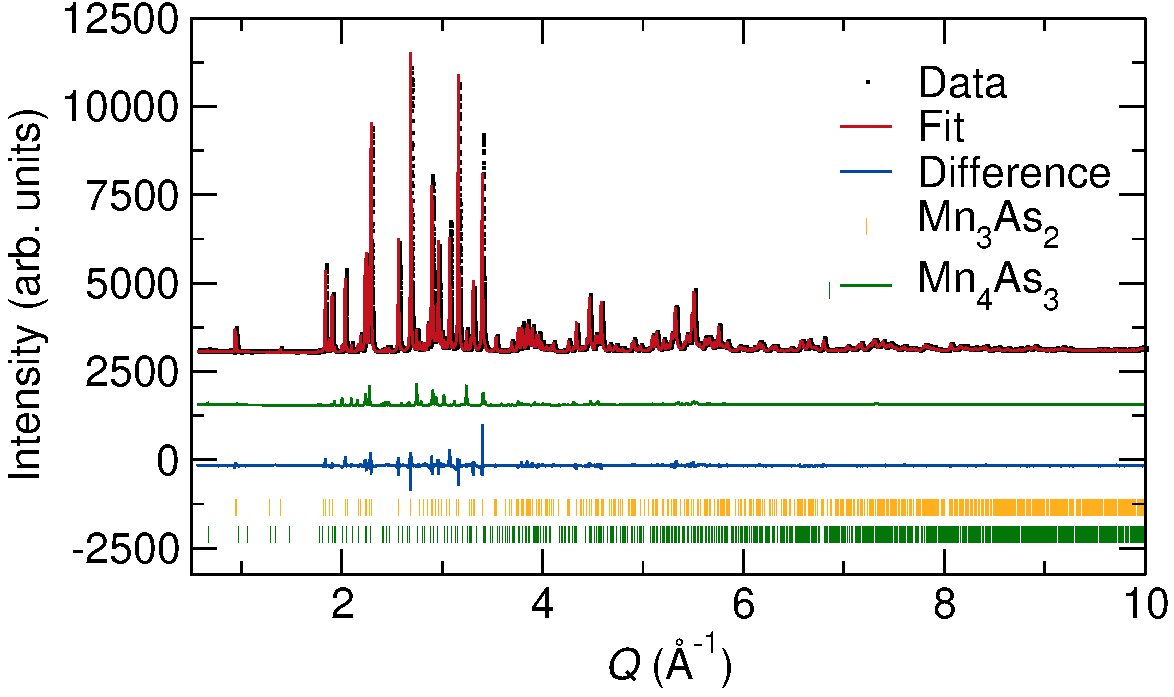
\includegraphics[width=0.7\columnwidth]{figures/ch6/6121_Mn3As2_cropped.pdf} \\
\caption{\label{fig:11BM_data}
Rietveld fit to the synchrotron powder x-ray diffraction data of Mn$_3$As$_2$ showed 7.4 wt.\% Mn$_4$As$_3$ impurity. The contribution of the Mn$_4$A$_3$ impurity phase to the diffraction data is also shown in the figure. This impurity was, however, not seen in the NPD data.
} 
\end{figure}

\begin{figure}
\centering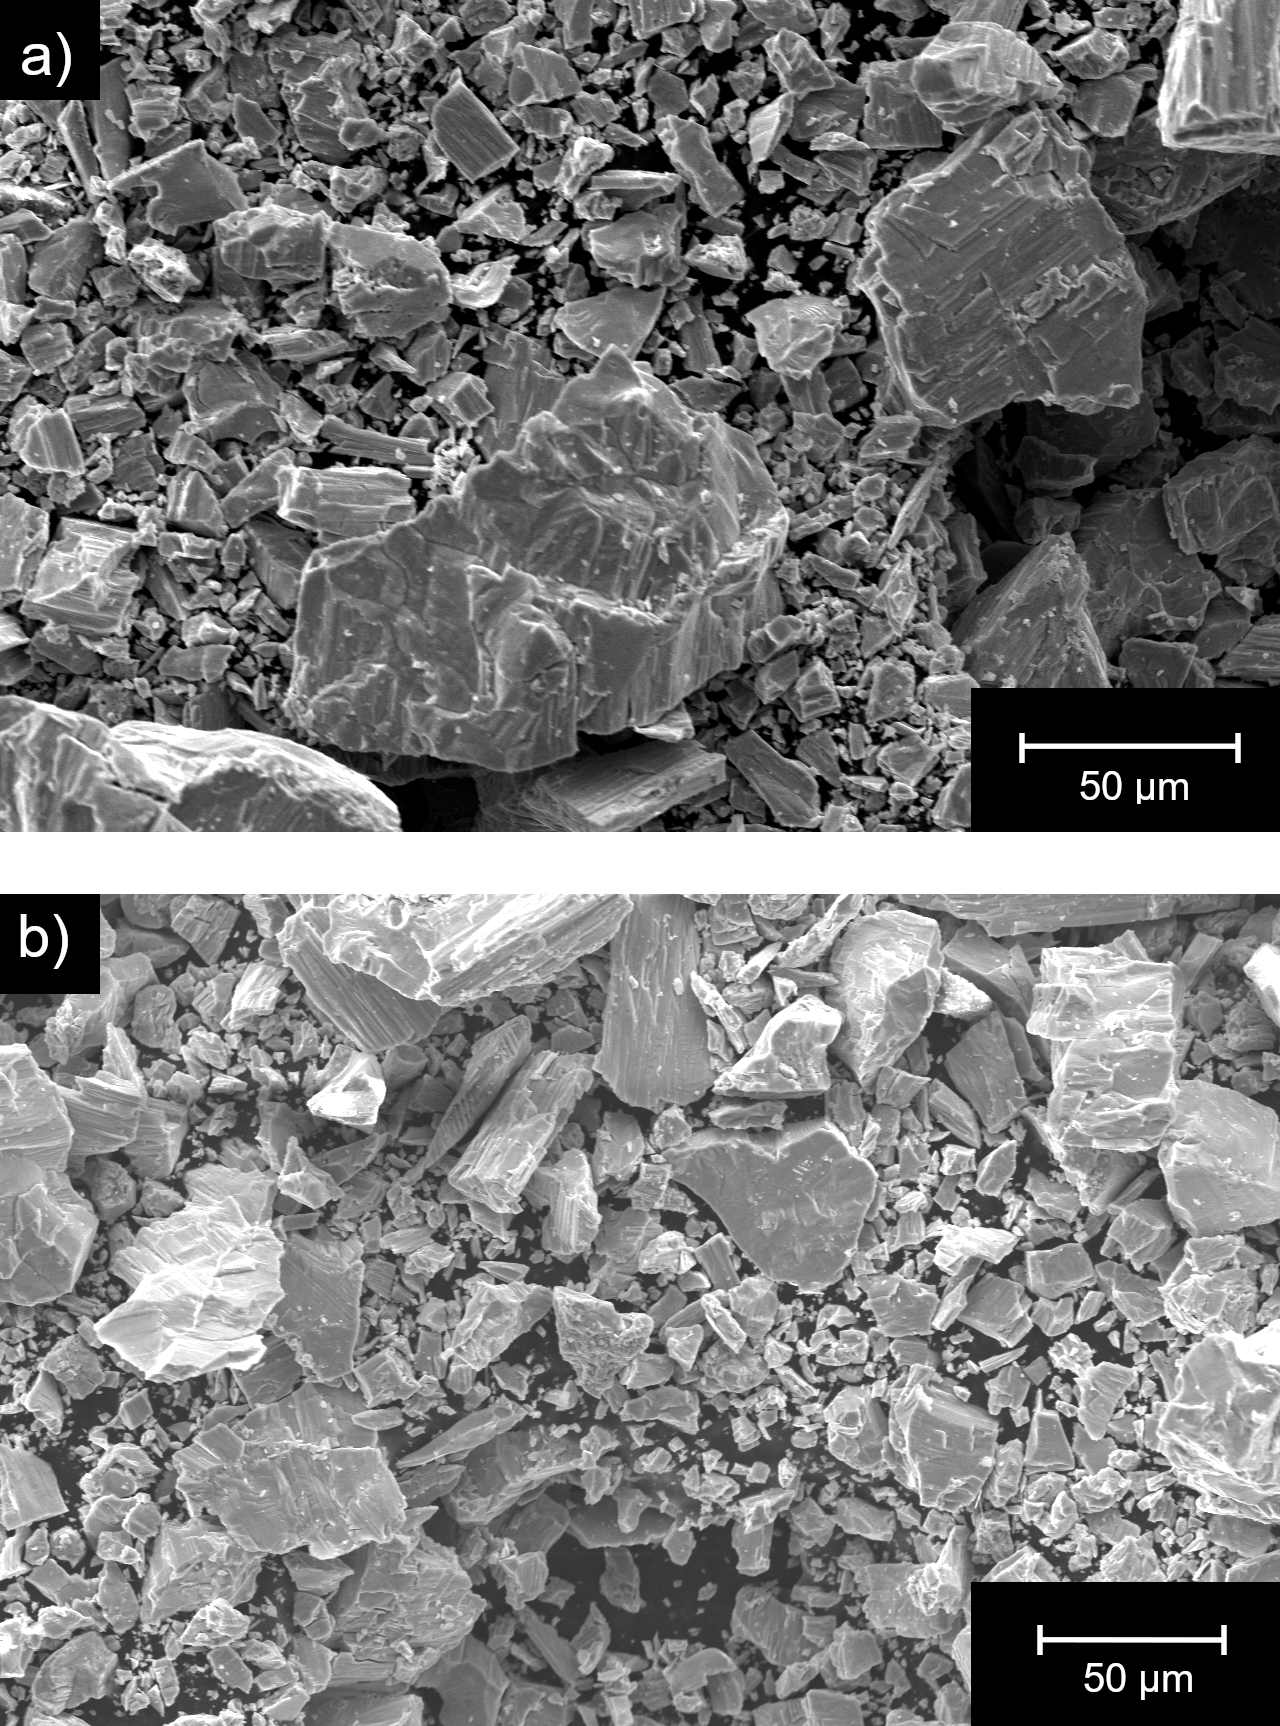
\includegraphics[width=0.7\columnwidth]{figures/ch6/Mn3As2_SEM_image.png} \\
\caption{\label{fig:SEM_image}
Scanning electron microscopy image of Mn$_3$As$_2$ crystals crushed from an ingot is shown in (a) and (b). Clear facets in the crystals indicate melting of the elemental powders during synthesis. 
} 
\end{figure}

\FloatBarrier

\begin{table}
\caption{\label{tab:refinement_250_K} 
The goodness of fit measured in terms of data residual (R$_{wp}$) and the unweighted phase residual of the magnetic phase (RF$^2$) for the four k-maximal subgroups at 250~K. 
}
\centering
\begin{tabular}{p{3cm}p{2.5cm}p{2.5cm}p{2.5cm}}
\hline\hline
\textbf{Space group} & \textbf{No.} & \textbf{R$_{wp}$ (\%)} & \textbf{RF$^2$ (\%)}\\
\hline\hline
$C2'/m'$ & $\#$12.62 & 5.954 &  19.579\\
$C2/m'$ & $\#$12.61 & 6.880 &  27.604\\
$C2'/m$ & $\#$12.60 & 6.186 &  21.937\\
\textbf{C2/m} & \textbf{\#12.58} & \textbf{5.087} &  \textbf{12.018}\\
\hline\hline
\end{tabular}
~\\
\end{table}

\begin{table}
\caption{\label{tab:refinement_3_K} 
The goodness of fit measured in terms of data residual (R$_{wp}$) and the unweighted phase residual of the magnetic phase (RF$^2$) for the four k-maximal subgroups containing the magnetic irrep mGM$_1^+$ at 3~K.
}
\centering
\begin{tabular}{p{3cm}p{2cm}p{3cm}p{2.5cm}p{2.5cm}}
\hline\hline
\textbf{Space group} & \textbf{No.} & \textbf{Translation vector} & \textbf{R$_{wp}$ (\%)} & \textbf{RF$^2$ (\%)}\\
\hline\hline
\textbf{C2/c} & \textbf{\#15.85} & \textbf{[0,0,0]} & \textbf{5.852} &  \textbf{6.773}\\
$C2/c$ & $\#$15.85 & $[0,0,\frac{1}{2}]$ & 6.112 &  8.079\\
$C2/m$ & $\#$12.58 & $[0,0,0]$ & 6.829 &  9.831\\
$C2/m$ & $\#$12.58 & $[0,0,\frac{1}{2}]$ & 6.719 &  8.486\\
\hline\hline
\end{tabular}
~\\
\end{table}

\begin{figure}
\centering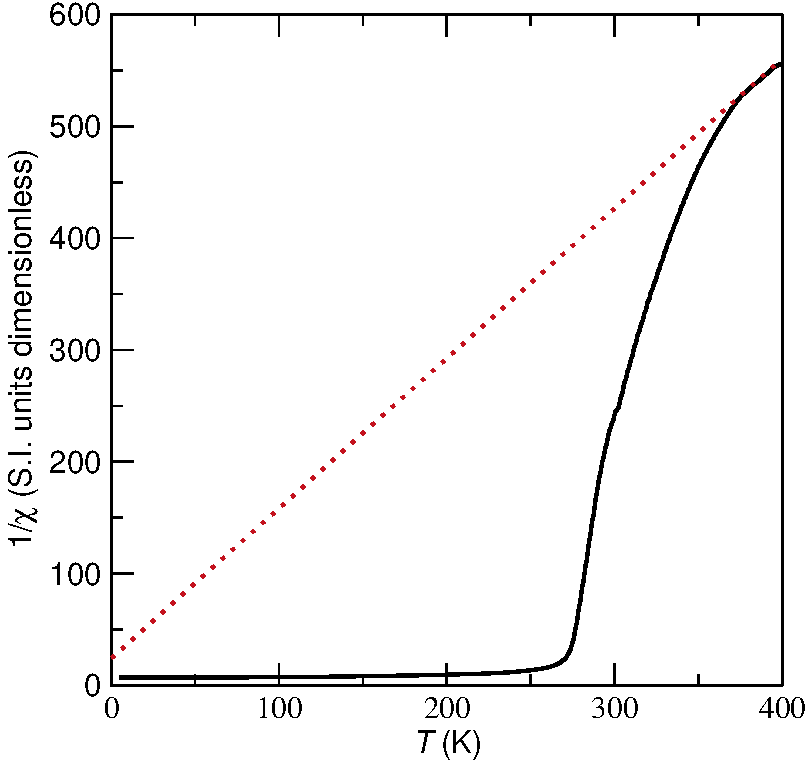
\includegraphics[width=0.6\columnwidth]{figures/ch6/FC_52A_inverse_cropped.pdf} \\
\caption{\label{fig:inverse_susceptibility}
Inverse susceptibility of the field cooling curve in Mn$_3$As$_2$. There are not enough data points at the linear regime to provide a Curie-Weiss fit. The red dotted line indicates the extrapolation from the visible linear regime.
} 
\end{figure}




%\iffalse

\FloatBarrier

%\Large 
\vspace{1em}
\begin{center}
\textbf{Cif file for Mn$_3$As$_2$ at 250~K}\\
\end{center}
\normalsize

\begin{verbatim}
data_As2_Mn3

# phase info for As2 Mn3 follows
_pd_phase_name  "As2 Mn3"
_cell_length_a  13.166866
_cell_length_b  3.681129
_cell_length_c  8.987757
_cell_angle_alpha  90
_cell_angle_beta   132.2013
_cell_angle_gamma  90
_cell_volume  322.708
_exptl_crystal_density_diffrn  3.3923
_symmetry_cell_setting  monoclinic
_parent_space_group.name_H-M_alt  "C 2/m"
_space_group_magn.name_BNS  "C 2/m"
_space_group.magn_point_group  2/m
loop_
    _space_group_symop_magn_operation.id
    _space_group_symop_magn_operation.xyz
     1  x,y,z,+1
     2  -x,y,-z,+1
     3  -x,-y,-z,+1
     4  x,-y,z,+1
     5  1/2+x,1/2+y,z,+1
     6  1/2-x,1/2+y,-z,+1
     7  1/2-x,1/2-y,-z,+1
     8  1/2+x,1/2-y,z,+1

# ATOMIC COORDINATES AND DISPLACEMENT PARAMETERS
loop_ 
   _atom_site_label
   _atom_site_type_symbol
   _atom_site_fract_x
   _atom_site_fract_y
   _atom_site_fract_z
   _atom_site_occupancy
   _atom_site_adp_type
   _atom_site_U_iso_or_equiv
   _atom_site_symmetry_multiplicity
Mn1    Mn2+ 0.30820     0.00000     0.68320     1.000      Uiso 0.011      4   
Mn2    Mn2+ 0.38883     0.00000     0.08690     1.000      Uiso 0.011      4   
Mn3    Mn2+ 0.00000     0.50000     0.50000     1.000      Uiso 0.016      2   
Mn4    Mn2+ 0.00000     0.00000     0.00000     1.000      Uiso 0.010      2   
As1    As   0.06069     0.00000     0.34317     1.000      Uiso 0.010      4   
As2    As   0.24682     0.00000     0.17768     1.000      Uiso 0.010      4   

loop_
   _atom_site_moment.label
   _atom_site_moment.crystalaxis_x
   _atom_site_moment.crystalaxis_y
   _atom_site_moment.crystalaxis_z
Mn1  0.0000      -0.52(9)    0.0000      
Mn2  0.0000      2.55(9)     0.0000      
Mn3  0.0000      -1.69(14)   0.0000      
Mn4  0.0000      0.59(6)     0.0000      

loop_  _atom_type_symbol _atom_type_number_in_cell
  As   8
  Mn   12

# Note that Z affects _cell_formula_sum and _weight
_cell_formula_units_Z  2
_chemical_formula_sum  "As4 Mn6"
_chemical_formula_weight  629.32

\end{verbatim}

%\Large 
\vspace{1em}
\begin{center}
\textbf{Cif file for Mn$_3$As$_2$ at 3~K}\\
\end{center}
\normalsize

\begin{verbatim}
data_As2_Mn3_mag_7

# phase info for As2 Mn3 follows
_pd_phase_name  "As2 Mn3"
_cell_length_a  13.085675
_cell_length_b  3.658847
_cell_length_c  17.832944
_cell_angle_alpha  90
_cell_angle_beta   132.1886
_cell_angle_gamma  90
_cell_volume  632.623
_exptl_crystal_density_diffrn  3.4609
_symmetry_cell_setting  monoclinic
_parent_space_group.name_H-M_alt  "C 2/c"
_space_group_magn.name_BNS  "C 2/c"
_space_group.magn_point_group  2/m
loop_
    _space_group_symop_magn_operation.id
    _space_group_symop_magn_operation.xyz
     1  x,y,z,+1
     2  -x,y,1/2-z,+1
     3  -x,-y,-z,+1
     4  x,-y,1/2+z,+1
     5  1/2+x,1/2+y,z,+1
     6  1/2-x,1/2+y,1/2-z,+1
     7  1/2-x,1/2-y,-z,+1
     8  1/2+x,1/2-y,1/2+z,+1

# ATOMIC COORDINATES AND DISPLACEMENT PARAMETERS
loop_ 
   _atom_site_label
   _atom_site_type_symbol
   _atom_site_fract_x
   _atom_site_fract_y
   _atom_site_fract_z
   _atom_site_occupancy
   _atom_site_adp_type
   _atom_site_U_iso_or_equiv
   _atom_site_symmetry_multiplicity
Mn1    Mn2+ 0.30820     0.00000     0.34160     1.000      Uiso 0.000      4   
Mn2    Mn2+ 0.38883     0.00000     0.04345     1.000      Uiso 0.000      4   
Mn3    Mn2+ 0.00000     0.50000     0.25000     1.000      Uiso 0.000      2   
Mn4    Mn2+ 0.00000     0.00000     0.00000     1.000      Uiso 0.000      2   
As1    As   0.06069     0.00000     0.171585     1.000      Uiso 0.000      4   
As2    As   0.24682     0.00000     0.08884     1.000      Uiso 0.000      4   

loop_
   _atom_site_moment.label
   _atom_site_moment.crystalaxis_x
   _atom_site_moment.crystalaxis_y
   _atom_site_moment.crystalaxis_z
Mn1  1.24(15)    -1.94(8)    2.27(11)    
Mn2  0.87(15)    2.28(7)     1.82(10)    
Mn3  0.0000      -4.48(13)   0.0000      
Mn4  -0.91(16)   1.21(6)     -0.56(11)   

loop_  _atom_type_symbol _atom_type_number_in_cell
  As   16
  Mn   24

# Note that Z affects _cell_formula_sum and _weight
_cell_formula_units_Z  4
_chemical_formula_sum  "As4 Mn6"
_chemical_formula_weight  629.32
\end{verbatim}
%\fi

%##################chapter 7
\chapter{Spin canting in tetragonal CuMnAs}

In progress



%##################chapter 8
\chapter{Strongly two-dimensional exchange interactions in the in-plane metallic antiferromagnet Fe$_2$As probed by inelastic neutron scattering}

\hfill \break

%\section{Copyrights and author contributions}

\href{https://doi.org/10.1103/PhysRevMaterials.4.114416}{Reprinted with permission from Manohar H. Karigerasi, Kisung Kang, Garrett E. Granroth, Arnab Banerjee, Andr\'e Schleife, and Daniel P. Shoemaker, Physical Review Materials 4, 114416 (2020). Copyright 2020 by the American Physical Society.} In this work, I synthesized single crystals of Fe$_2$As, carried out the alignment of the samples and measured inelastic neutron scattering (INS) spectra at Oak Ridge National Laboratory. I was also responsible for slicing and cutting INS data using mantidplot, simulating magnon spectra using SpinW and refining the magnon spectra to get exchange coupling values. Kisung Kang did DFT simulations to obtain phonon spectra and simulated phonon intensities using OCLIMAX. I wrote the paper with help from coauthors.


%\begin{abstract}

\section{Abstract}
To understand spin interactions in materials of the Cu$_2$Sb structure type, inelastic neutron scattering of Fe$_2$As single crystals was examined at different temperatures and incident neutron energies. The experimental phonon spectra match well with the simulated phonon spectra obtained from density functional theory (DFT) calculations. The measured magnon spectra were compared to the simulated magnon spectra obtained via linear spin wave theory with the exchange coupling constants calculated using the spin polarized, relativistic Korringa-Kohn-Rostoker method in Zhang \emph{et al}. (2013). The simulated magnon spectra broadly agree with the experimental data although, the energy values are underestimated along the $K$ direction. Exchange coupling constants between Fe atoms were refined by fits to the experimental magnon spectra, revealing stronger nearest neighbor Fe1-Fe1 exchange coupling than previously reported. The strength of this exchange coupling is almost an order of magnitude higher than other exchange interactions despite the three-dimensional nature of the phonon interactions. The lack of scattering intensity at energies above 60~meV makes unconstrained determination of the full set of exchange interactions difficult, which may be a fundamental challenge in metallic antiferromagnets.


%\end{abstract}

%\fi

\section{Introduction} 

With recent interest towards understanding the possibility of electrical switching behavior in metallic antiferromagnets \cite{Baltz2018,Siddiqui2020,Jungfleisch2018,Zelezny2018}, notably in CuMnAs \cite{Wadley2016,Grzybowski2017,Wadley2018,Matalla-Wagner2019} and Mn$_2$Au \cite{Meinert2018,Bodnar2019}, the relationships between their static magnetic orders \cite{Wadley2013,Hills2015,Wadley2015,Saidl2017}, in some cases are quite recently determined, and their spin dynamics \cite{Grzybowski2017,Bodnar2019,Yang2019,Yang2020} are of crucial interest. CuMnAs is a member of a larger family of easy-plane metallic antiferromagnets in the Cu$_2$Sb structure type \cite{Nateprov2011,Wadley2013}, which includes Cr$_2$As \cite{Yuzuri1960Cr2As}, Mn$_2$As \cite{Yuzuri1960}, and Fe$_2$As \cite{Katsuraki1966}.
The proposed switching involves a field-like torque from exchange interactions between the carrier spins and the moments of the magnetic atoms. The non-equilibrium current-induced spin polarization is staggered across the two sublattices and exerts a uniform torque on the N\'{e}el vector \cite{Zelezny2014,Zelezny2017,Wadley2016}.
While the static spin arrangements of these easy-plane antiferromagnets are known, the underlying energy scales and dynamics are less so. 
Determination of fundamental exchange and anisotropy energies are essential to understand what energy barriers and resonances may dominate in these materials.


\begin{figure}
\centering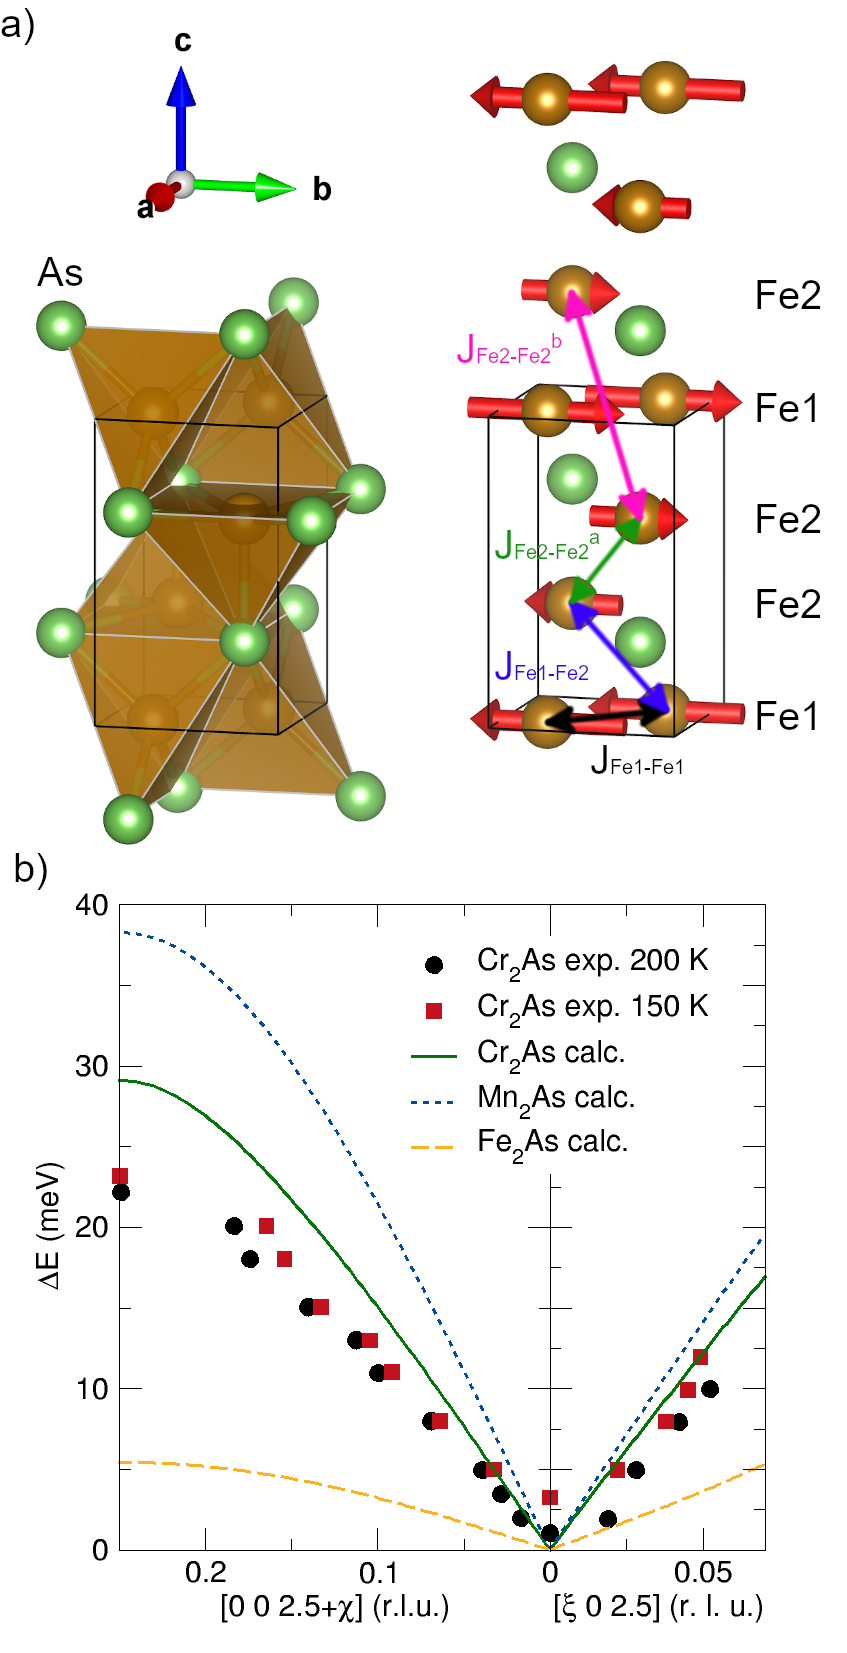
\includegraphics[width=0.65\columnwidth]{figures/ch8/Cr2As_INS_magnetic_structure.png} \\
\caption{\label{fig:Cr2As_plot}
The chemical structure of Fe$_2$As (left) showing the FeAs$_4$ tetrahedral and FeAs$_5$ square pyramidal units and the Fe$_2$As magnetic structure (right) with Fe-Fe exchange pathways are shown in (a). Black, blue, green and pink double headed arrows represent Fe1-Fe1, Fe1-Fe2, Fe2-Fe2 nearest-neighbor, and Fe2-Fe2 next-nearest-neighbor interactions, respectively. Comparison between the magnon spectra calculated using the linear spin wave theory from exchange coupling values in reference \citenum{Zhang2013} and the experimental INS values in reference \citenum{Ishimoto1995} are shown in (b) for Cr$_2$As. Also overlaid are the SPRKKR-derived magnon spectra of Mn$_2$As and Fe$_2$As \cite{Zhang2013}. 
} 
\end{figure}

Fe$_2$As contains two different metal atom sites, Fe1 and Fe2, as shown in Fig. \ref{fig:Cr2As_plot}(a). Fe1 atoms are centered in FeAs$_4$ tetrahedra, which are arranged to form a square planar grid similar to the anti-PbO type Fe--As layers in iron arsenide superconductors. 
Fe2 atoms form edge-sharing FeAs$_5$ square pyramids. 
Fe$_2$As has a magnetic unit cell that is twice the length of its chemical unit cell along $c$ \cite{Zhang2013,Katsuraki1966}.  It is the Fe moments that we are concerned about in the magnon spectrum, but the As contributes to the phonons. The magnetic ground state of Fe$_2$As was determined using single crystal and powder neutron diffraction and consists of alternating slabs of ferromagnetically aligned trilayers of Fe atom planes (Fe2--Fe1--Fe2) as shown in Fig. \ref{fig:Cr2As_plot}(a) \cite{Katsuraki1966}.
Exchange interactions obtained from  spin polarized, relativistic Korringa-Kohn-Rostoker (SPRKKR)  calculations indicate a strong nearest-neighbor ferromagnetic (FM) Fe1-Fe1 coupling and a weak nearest-neighbor antiferromagnetic (AFM) Fe2-Fe2 interaction \cite{Zhang2013}.
The Fe-Fe exchange interactions, modeled using SPRKKR calculations, have been explained based on crystal orbital Hamilton population (COHP) curves. The strong Fe1-Fe1 exchange coupling is a result of a strong Fe1-Fe1 anti-bonding orbital overlap as opposed to a weak non-bonding orbital overlap in Fe2-Fe2 nearest neighbor exchange interaction. This case is opposite for Mn$_2$As \cite{Zhang2013}.
Unlike Fe$_2$As, there is frustration in Mn$_2$As and Cr$_2$As and the magnetic ground state is decided by the dominant exchange interactions \cite{Zhang2013}.


To date, the only direct measurements of exchange interactions in M$_2$As compounds are triple-axis inelastic neutron scattering (INS) measurements on Cr$_2$As single crystals \cite{Yuzuri1960,Ishimoto1995}.
Magnon spectra calculated from linear spin wave theory using SPRKKR-derived exchange coupling values from Zhang \emph{et al}.\ are plotted on the experimental points from Ishimoto, et al.\ in Fig. \ref{fig:Cr2As_plot}(b) \cite{Zhang2013,Ishimoto1995}. The experimental magnon spectra roughly agrees with the calculated magnon spectra for the slice plotted in the limited range of reciprocal space. The corresponding magnon spectra for Fe$_2$As and Mn$_2$As from exchange constants in Zhang \emph{et al}.\ are also shown in Fig. \ref{fig:Cr2As_plot}(b). 
Since the transition temperature (T$_N$ or T$_C$) is generally proportional to the strength of exchange interactions in a material \cite{Krishnan2016}, the slope of the spin waves along both $H$ and $L$ direction is consistent with T$_N$ of the materials (T$_N$ = 573~K, 393~K and 373~K for Mn$_2$As, Cr$_2$As and Fe$_2$As respectively) \cite{Zhang2013}.
Torque magnetometry measurements have been carried out on Fe$_2$As single crystals at different temperatures to determine the four-fold in-plane anisotropy constants \cite{Yang2020,Achiwa1967}. From these measurements, it is clear that the in-plane anisotropy in Fe$_2$As is very small ($<$~1~$\mu$eV) and cannot be resolved using INS measurements. 

Given the technological implications of possible data storage, and the limited momentum space previously examined, a full picture of magnon spectra in metallic antiferromagnets is needed to determine the exchange interactions, and to validate methods of their calculation. Such direct verification has been elusive, and is especially important in highly-correlated 3$d$ systems.
Fe$_2$As single crystals have been grown in centimeter scale \cite{Katsuraki1966},  making it an ideal candidate to study magnon spectra. In this paper, we report the growth of large Fe$_2$As single crystals and carry out time-of-flight neutron scattering measurements at different temperatures. We identify phonon intensities by comparing with density functional theory-calculated phonon spectra and compare magnon spectra with the reported exchange coupling values. Finally, we refine the exchange coupling values against the INS data to obtain accurate values.


\section{Methods}

\begin{figure}
\centering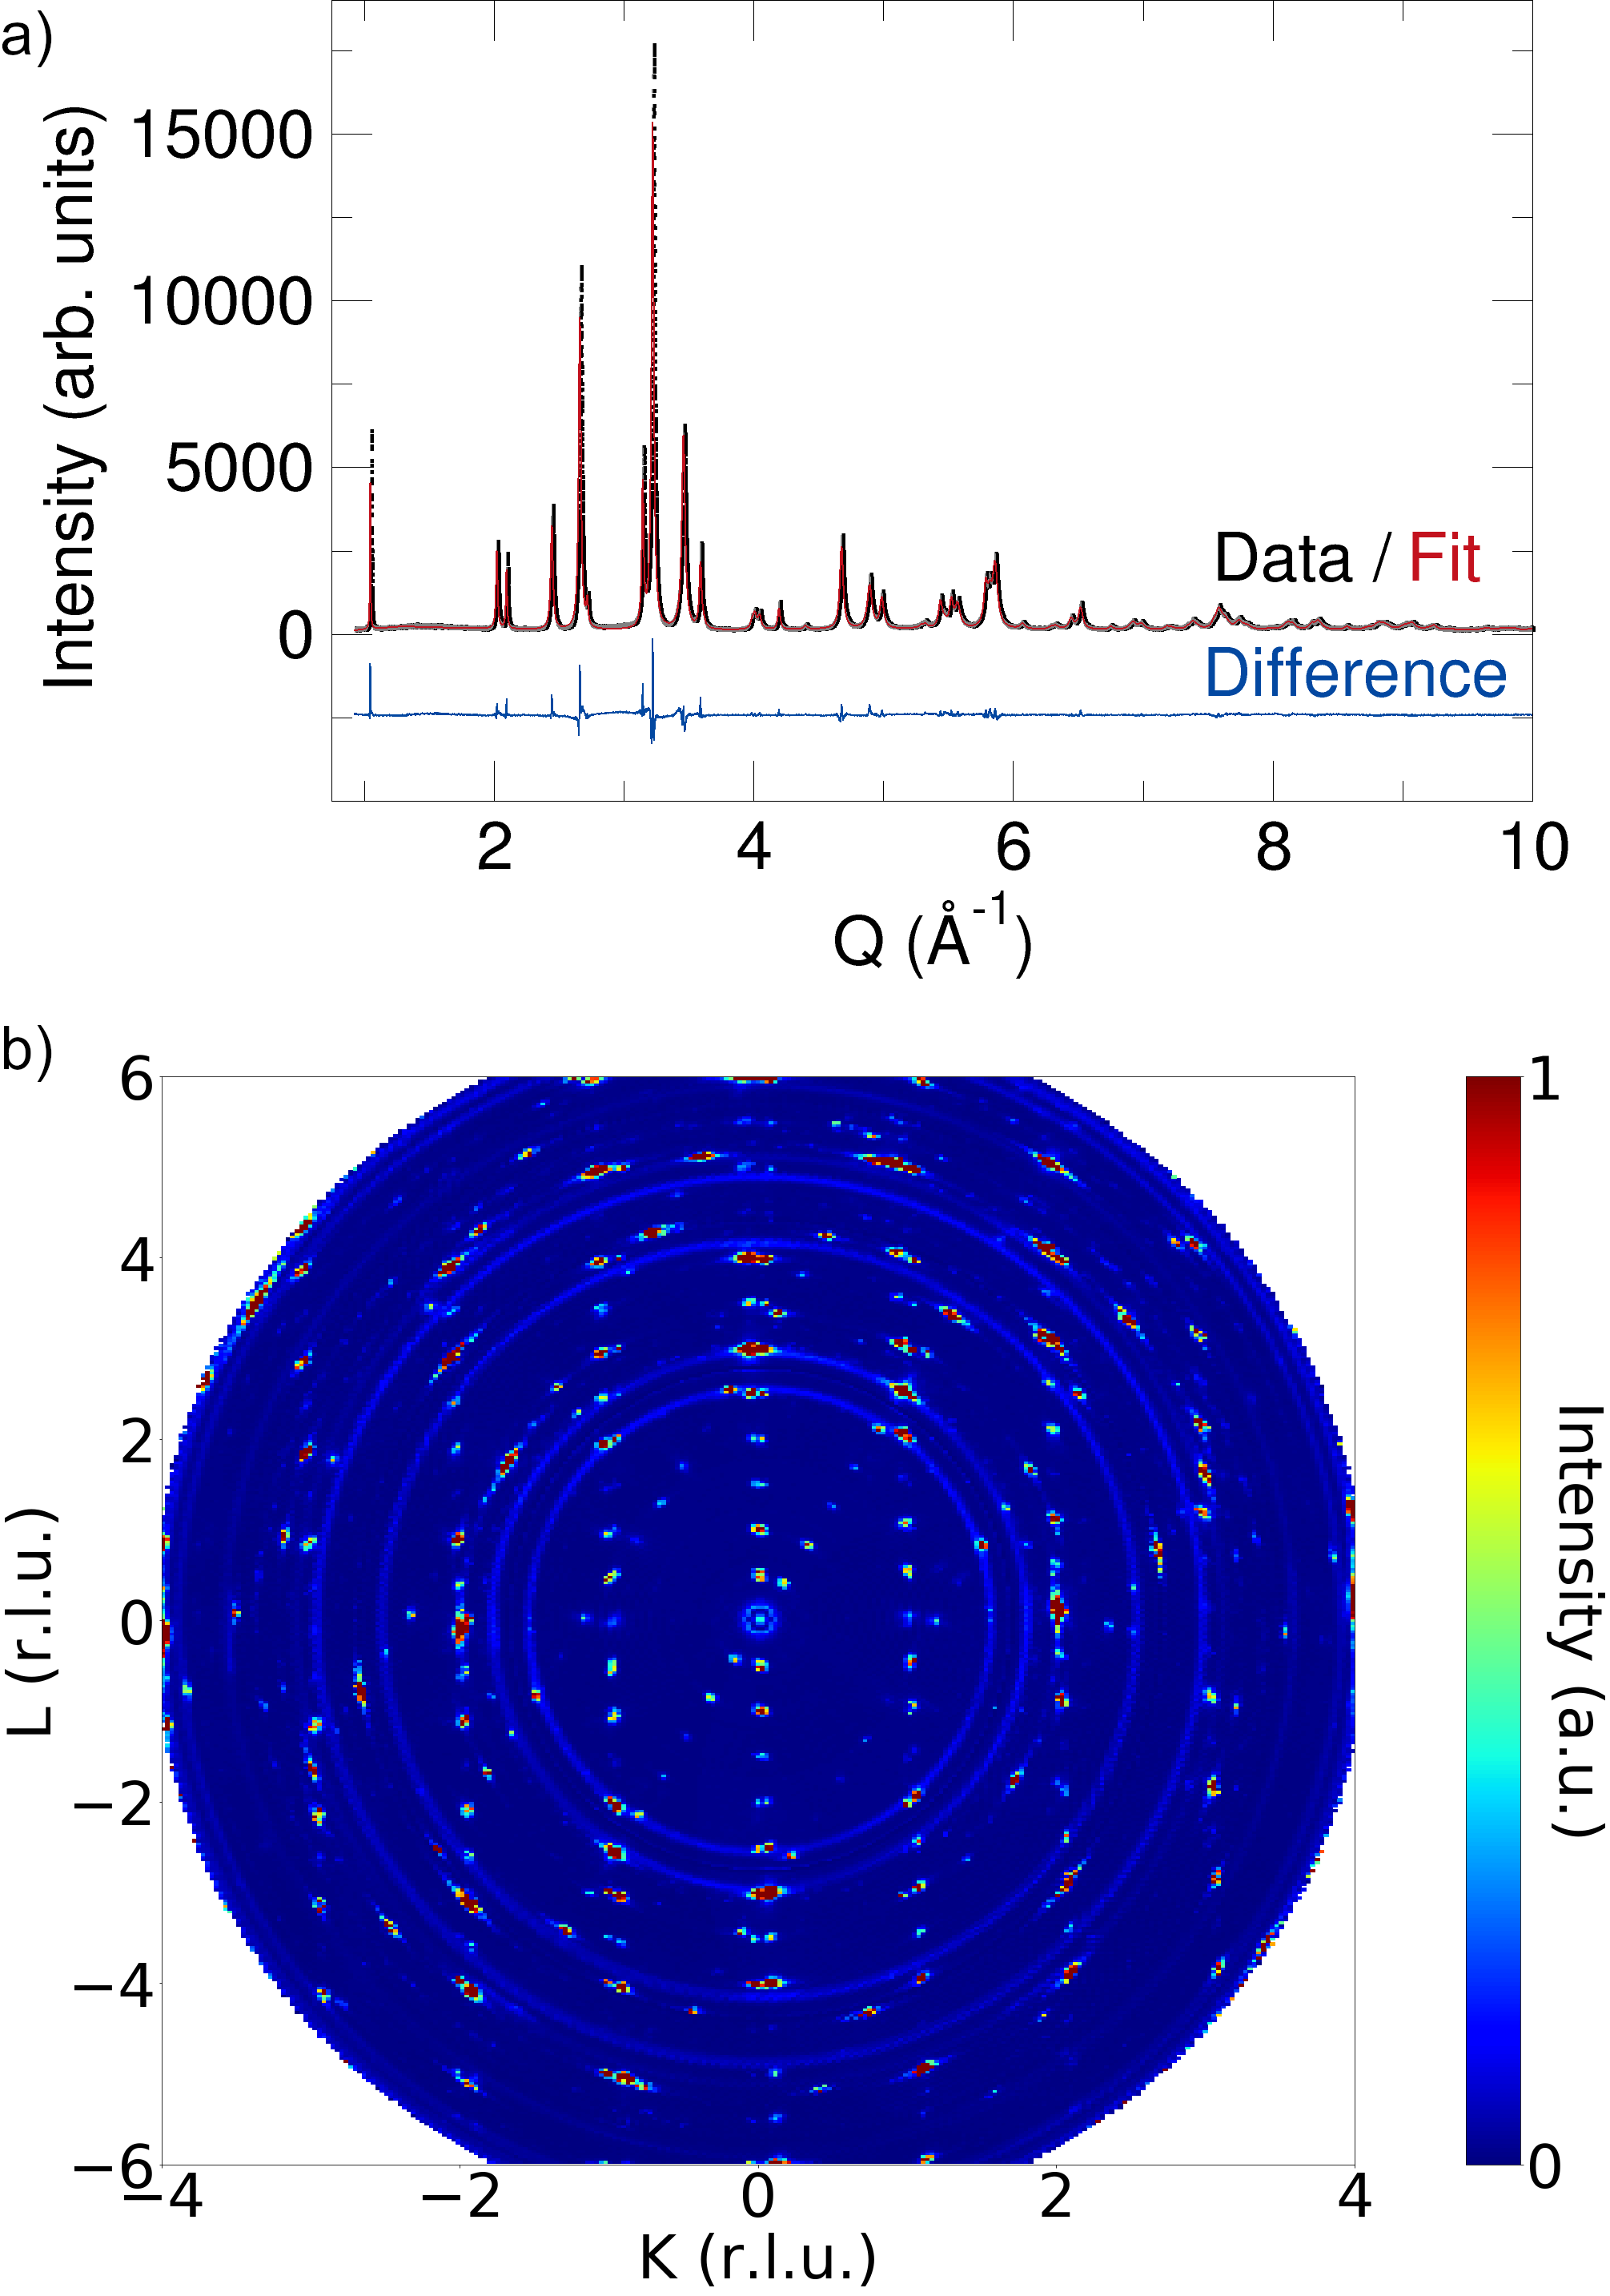
\includegraphics[width=0.65\columnwidth]{figures/ch8/11BM_refinement_elastic_slice.png} \\
\caption{\label{fig:photo_11_BM}
The Rietveld-refined fit to the synchrotron powder x-ray diffraction data of Fe$_2$As is shown in (a). 
The elastic neutron scattering slice along $K$ and $L$ for $H$ integrated from -0.2 to 0.2 is shown in (b) for $E_i$ = 30~meV. 
}

\end{figure}


\begin{figure}
\centering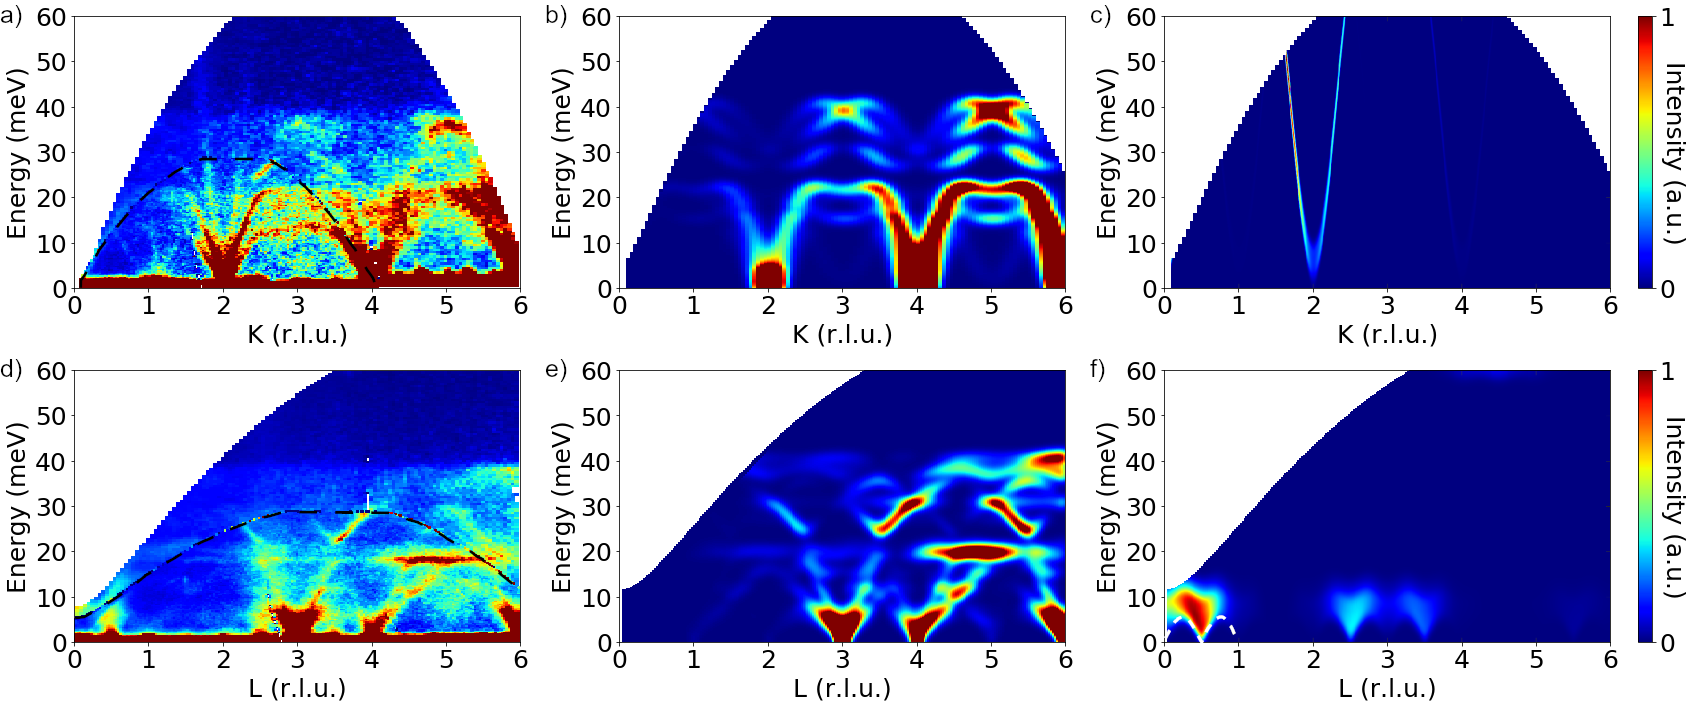
\includegraphics[width=\columnwidth]{figures/ch8/phonon_spectra_magnon_spectra_combined.png} \\
\caption{\label{fig:phonon_magnon_spectra}
INS data of Fe$_2$As measured at 5 K along $K$ with $H$ and $L$ integrated from -0.1 to 0.1 is shown in (a) and along $L$ with $H$ and $K$ integrated from -0.2 to 0.2 is shown in (d). The data with $E_i = 30$~meV (below black dashed lines) have been overlaid on the data with $E_i = 70$~meV in (a) and (d). Panels (b) and (e) show the corresponding simulated phonon spectra obtained from DFT calculations. Panels (c) and (f) show the corresponding simulated magnon spectra derived from exchange constants in reference \citenum{Zhang2013}. The intensities in (b) and (e) have been averaged over 9 equally-spaced phonon spectra in the experimental width along other two $Q$ directions. Similarly, the magnon spectra in (c) and (f) have been averaged over every 0.025 reciprocal lattice units between -0.1 to 0.1 in the other $Q$ directions. The white dashed lines in (f) indicate the calculated magnon spectrum along the [0 0 $L$] direction.
}
\end{figure}


Large crystals (about 1 cm in length with a mass of about 3 g) were grown from the elements. 
Fe ($>$99.99\% metals basis) and As (99.9999\% metals basis) powders were mixed in 2:1 molar ratio inside an Ar filled glove box and vacuum sealed inside a 7 mm inner diameter quartz tube.
The tube was heated to 600$^{\circ}$C at 1$^{\circ}$C/min and held for 6 hours, heated to 975$^{\circ}$C at 1$^{\circ}$C/min and held for 1 hour, cooled to 900$^{\circ}$C at 1$^{\circ}$C/min and held for 1 hour, then allowed to furnace cool at approximately 10$^{\circ}$C/min to room temperature. The resulting crystals were silver-black in color and produced a mirror like finish when cleaved as shown in Fig. \ref{fig:crystal_array}. The phase purity  was confirmed using synchrotron powder X-ray diffraction  at beamline 11-BM of the Advanced Photon Source in Argonne National Laboratory. Rietveld analysis of the synchrotron data is shown in Fig. \ref{fig:photo_11_BM}(a).



The large Fe$_2$As single crystals were gently tapped using a pestle to reveal sharp cleaved surfaces along the $ab$ plane.
Five cleaved crystals of Fe$_2$As, with a total mass of 9 g, were co-aligned onto the base of an Al can and checked with a Multiwire Laue setup at the Spallation Neutron Source (SNS) \cite{mason2006spallation} in Oak Ridge National Laboratory (ORNL). The individual crystals were wrapped in Al foil and sewed to Al shims using Al wires as shown in Fig. \ref{fig:crystal_array}(a) and (b).
One of the five crystals became misaligned, which can be seen in the elastic-scattering slice along $KL$ plane in Fig. \ref{fig:photo_11_BM}(b).
Accordingly, regions are selected here from constant energy slices where the effect of the misaligned crystal is minimized. The simulated phonon and magnon spectra do not include the intensity from the misaligned crystal to provide better clarity of the data. Details regarding the intensities from misalignment are provided in the Supplementary section.

The inelastic neutron scattering measurement of Fe$_2$As
was carried out at the ARCS (Wide Angular-Range Chopper Spectrometer) beamline \cite{ doi:10.1063/1.3680104} of the SNS at ORNL. For measurements at  base temperature (about 5~K) and 200~K, the can containing the crystal array was mounted onto a closed cycle refrigerator (CCR) such that the horizontal $(0KL)$ plane was perpendicular to the axis of rotation. For measurement at 400~K (above $T_N$ = 353~K), the crystal array was removed from the can and mounted directly to the CCR. The crystal array was rotated by 360$^{\circ}$ at 1$^{\circ}$ steps in the horizontal plane.
At base temperature, measurements were performed at $E_i = 30$, 70, 200 and 300~meV.  Additional measurements at 70~meV were performed at 200 and 400~K.
Chopper settings were chosen to provide the optimum $Q$ range and resolution conditions, based on Lin, et al. (2019) \cite{Lin2019}. For $E_i = 30$ and  70 meV, the 100~meV Fermi chopper was spun at 300 and 480~Hz respectively.  For $E_i = 200$ and 300~meV, the 700~meV chopper was spun at 540 and 420~Hz respectively.  Both choppers have 1.5~mm slit spacing.


Data processing (slicing, folding, and gaussian smoothing) was performed using \textsc{Mantid} \cite{Arnold2014}. The reciprocal lattice units for Fe$_2$As along $K$ (same as $H$) and $L$ correspond to 1.73~\AA$^{-1}$~and 1.05~\AA$^{-1}$, respectively.
Simulated magnon spectra were calculated and refined using the \textsc{SpinW MATLAB} library module, which can solve the spin Hamiltonian using numerical methods and linear spin wave theory \cite{Toth_2015}. 
In \textsc{SpinW}, we use a spin-only ($S$)  Hamiltonian based on isotropic exchange interactions $J_{ij}$: $ H = \sum_{i,j} S_i J_{ij} S_j$.
    

Density-functional theory (DFT) calculations were performed using the Vienna \emph{Ab-Initio} Simulation Package \cite{Kresse:1996,Kresse:1999} (VASP). The projector-augmented wave \cite{Blochl:1994} (PAW) scheme was used to describe the electron-ion interaction. Kohn-Sham states are expanded into a plane-wave basis up to a kinetic-energy cutoff of 600 eV. A $15\,\times\,15\,\times\,5$  Monkhorst-Pack (MP) \cite{Monkhorst:1976} $\mathbf{k}$-point grid was used to sample the Brillouin zone. Exchange and correlation was described using the generalized-gradient approximation (GGA) in the formulation by Perdew, Burke, and Ernzerhof.\cite{Perdew:1997} The phonon dispersion was computed with the \textsc{phonopy} package \cite{Phonopy:2015} based on the finite displacement method with total energies from DFT. This calculation used a $3\,\times\,3\,\times\,2$ supercell and a $4\,\times\,4\,\times\,4$ MP $\mathbf{k}$-point grid. The simulated phonon INS spectra were computed using \textsc{OCLIMAX} \cite{Cheng2019} using all phonon eigenvalues from DFT, represented on a reciprocal-space grid. All simulations, in particular all atomic geometry relaxations and phonon dispersion calculations, were performed including noncollinear magnetism and the fully relativistic spin-orbit coupling interaction \cite{Steiner2016}. The instrument parameters used in \textsc{OCLIMAX} correspond to a high resolution measurement at ARCS with an $E_i = 70$~meV.

\begin{figure}
\centering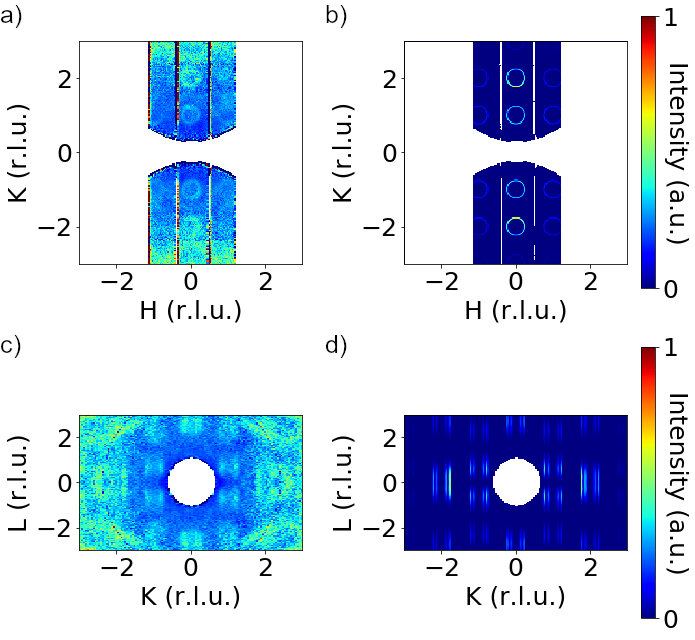
\includegraphics[width=0.7\columnwidth]{figures/ch8/constant_energy_slices.png} \\
\caption{\label{fig:constant_energy_slices}
Constant-energy INS data reveal magnons most clearly with $E$ integrated from 25 meV to 30 meV for (a) the $H-K$ plane with $L$ integrated from -1 to 1 and (c) $K-L$ plane with $H$ integrated from -0.2 to 0.2 and folded along $L$. Panels (b) and (d) show the corresponding simulated magnon spectra using exchange constants from Zhang \emph{et al}. \cite{Zhang2013} with the same $E$ integration and the orthogonal $Q$ direction summed every 0.1 along the experimental width.
}
\end{figure}


\section{Results and Discussion}



Fig.s \ref{fig:phonon_magnon_spectra}(a) and \ref{fig:phonon_magnon_spectra}(d) show the inelastic neutron scattering spectra of Fe$_2$As at $T = 5$~K and $E_i =$~70 meV. The corresponding simulated phonon spectra are shown in Fig.s \ref{fig:phonon_magnon_spectra}(b) and \ref{fig:phonon_magnon_spectra}(e), respectively. Clearly, the phonon contributions form the majority of the experimental spectra, with intensity increasing with $Q$. 
The weak intensity below $E = 10$~meV  at $K = 1$ and $K = 3$ in the experimental data in Fig. \ref{fig:phonon_magnon_spectra}(a) is an overlapping phonon band from a misaligned crystal, as seen in Fig. \ref{fig:photo_11_BM}(b) and Fig. \ref{fig:misaligned_elastic}(b). The group velocities extracted from the three acoustic phonon modes near $\Gamma$ along $K$ (1.215, 2.903, 5.002 km/s) and $L$ (1.745, 1.846, 5.762 km/s) indicate stiffness constants that are the same order of magnitude along  perpendicular directions.




The clearest discrepancy between the experimental spectrum in Fig. \ref{fig:phonon_magnon_spectra}(a) and the calculated phonon spectrum in Fig. \ref{fig:phonon_magnon_spectra}(b) is the steep excitation arising from $K = 2$. To a first approximation, this magnon mode agrees with the calculated magnon spectrum in Fig. \ref{fig:phonon_magnon_spectra}(c), which has a single excitation visible at $K = 2$. When viewed along $a$, the presence of two Fe atoms along $b$ and three Fe atoms along $c$ in the Fe$_2$As chemical unit cell means that the periodicities of the observed phonon and magnon spectra are 2 and 3 along $[0K0]$ and $[00L]$, respectively.

\begin{table}
\caption{\label{tab:Jvalues} 
Exchange coupling constants (in meV) obtained by fitting the experimental magnon spectra along $K$. 
}
\centering
\begin{tabular}{p{3cm}p{2cm}p{2cm}p{2cm}p{2cm}p{2cm}}
\hline\hline
	&  \textbf{Fe1-Fe1 (J$_{Fe1-Fe1}$)} & \textbf{Fe1-Fe2 (J$_{Fe1-Fe2}$)} & \textbf{Fe2-Fe2 (J$_{Fe2-Fe2^a}$)} & \textbf{Fe2-Fe2* (J$_{Fe2-Fe2^b}$)} & \textbf{Reduced $\chi^2$} \\

\textbf{Distance (\AA)} & 2.547 & 2.6859 & 3.2774 & 4.7160\\
\hline\hline
\textbf{Zhang \emph{et al}.} & -25.4 & -6.52 & 3.52 & -8.52 & 54.55\\
\hline
\textbf{Fit} & -48.37(25) & -4.42(25) & 5.16(12) & -8.52 & 6.47\\
\hline\hline
\end{tabular}
~\\
\end{table}



From DFT SPRKKR-derived exchange coupling values in Zhang \emph{et al}.,\cite{Zhang2013} magnon spectra were calculated using the linear spin wave theory and simulated with an energy binning of 3~meV, which corresponds to our experimental resolution near the elastic limit with $E_i$~=~70~meV. Fig.s \ref{fig:phonon_magnon_spectra}(c) and \ref{fig:phonon_magnon_spectra}(f) show the magnon spectra along $K$ and $L$ directions, respectively. All the intensities in Fig.s \ref{fig:phonon_magnon_spectra}(a) and \ref{fig:phonon_magnon_spectra}(d) are accounted for in the simulated phonon and magnon spectra. The spectral weight of the magnons is mostly negligible along $L$ except for the locations shown in Fig. \ref{fig:phonon_magnon_spectra}(f). Constant-energy slices at $E$~=~25~meV in the $H-K$ and $K-L$ planes are shown in Fig. \ref{fig:constant_energy_slices}(a,c). The simulated magnon spectra in Fig. \ref{fig:constant_energy_slices}(b,d) give excellent reproduction of the corresponding INS data. Smaller magnon circles in Fig. \ref{fig:constant_energy_slices}(a) as compared to the ones in Fig. \ref{fig:constant_energy_slices}(b) indicate the possibility of stronger in-plane exchange interactions than those reported in Zhang \emph{et al}.\cite{Zhang2013}


On quick inspection of Fig. \ref{fig:phonon_magnon_spectra}(c), the energy dependence along $K$ appears to be a simple 1-D Heisenberg FM spin chain where the magnon spectrum varies as $1 - \textrm{cos} (Ks)$ \cite{Stancil}, $s$ being the interatomic spacing for the FM chain along $b$. Since the spins in Fe$_2$As are all aligned parallel to each other along $b$, the exchange interactions are consistent with the ground state. However, the spectrum is repeated every two reciprocal lattice units along $K$ since the unit cell contains two Fe atoms along $b$. The magnon spectrum along $L$ in Fig. \ref{fig:phonon_magnon_spectra}(f) has a similar $|\textrm{sin}(Ls)|$ dependence as seen in a 1-D Heisenberg AFM spin chain where $s$ is the interatomic spacing for the AFM chain along $c$. Unlike a 1-D Heisenberg AFM spin chain, however, Fe$_2$As contains AFM-stacked trilayers of Fe atoms. 
The dispersion of the spin waves in Fig. \ref{fig:phonon_magnon_spectra}(a,d) indicate a strong FM coupling along $b$ and weak trilayer AFM coupling along $c$ as also confirmed from the exchange coupling values in Zhang et. al. (2013) \cite{Zhang2013} in Table \ref{tab:Jvalues}.


From torque magnetometry measurements in the $ab$ plane, the four-fold in-plane anisotropy in Fe$_2$As at liquid nitrogen temperatures was reported to be around 700~erg/g, which is~0.3 $\mu$eV/cell \cite{Achiwa1967}.
Recent measurements at 5~K conclude that this quantity is much lower than previously reported at 0.074~$\mu$eV/cell (150 J/m$^3$) and it deceases to zero at around 150 K \cite{Yang2020}.
The out-of-plane 2-fold anisotropy value was estimated using DFT calculations to be 410 $\mu$eV/cell (-830 kJ/m$^3$).\cite{Yang2020} A similarly small anisotropy was reported for CuMnAs using relativistic calculations where the in-plane anisotropy was calculated to be less than 1 $\mu$eV/cell and the out-of-plane value was reported to be 127 $\mu$eV/cell \cite{Wadley2015}. Our ARCS experimental resolution in $E$ near the elastic limit is around  3 - 5\% of $E_i$, so anisotropy in Fe$_2$As can be neglected. 


The calculated magnon spectra using exchange constants from Zhang \emph{et al}. \cite{Zhang2013} underestimate the magnon energy along $K$ (by about 24\% at $K = 1.25$).
Ideally, refinement of the magnon spectra with \textsc{SpinW} \cite{Toth_2015} should extract more accurate exchange constant values.
Along $L$, as shown in Fig. \ref{fig:phonon_magnon_spectra}(f), even small integration of $Q$ in the orthogonal directions causes significant bleeding over of intensity due to the steep magnon modes in the $H$ and $K$ directions. The same effect is seen for $K = 1$, shown in Fig. \ref{fig:phonon_magnon_spectra_01L}(c).
Hence, the calculated magnon spectra in Fig. \ref{fig:phonon_magnon_spectra}(f) was assumed to be correct and points were taken from the calculated magnon spectra along $L$. This ensures a net weak AFM coupling along $L$ for the purpose of refinement.
Higher-energy INS data collected at 5~K using $E_i=200$~meV and 300~meV are shown in Fig.s \ref{fig:high_energy_data}(a,b). As shown in Fig.s \ref{fig:high_energy_data}, we see that the scattering extends up beyond 120~meV. We did not use this data in the fits as the itinerant nature of the moments at this energy leads to significant damping that blurs the mode position.  Nevertheless the results obtained from the fits are consistent with this scattering. Only the INS data obtained from $E_i=30$~meV and 70~meV  were considered for refinement.
From high temperature susceptibility measurements of Fe$_2$As \cite{Katsuraki1966}, the effective total moment per Fe is estimated as 4.66~$\upmu_\text{B}$ averaged over the two sublattices. The ordered moment, which is estimated by neutron diffraction in Fe1~=~0.95~$\upmu_\text{B}$ and Fe2~=~1.52~$\upmu_\text{B}$, is lower than 4.66~$\upmu_\text{B}$ \cite{Katsuraki1966,Zhang2013}. So, the rest of the moment can be assumed to be itinerant or short-ranged. The extracted average total moment of the Fe sublattices seems unusually high and well-calibrated high temperature susceptibility measurements are thus warranted.
The set of experimental data points used to refine the exchange interactions is shown in Fig. \ref{fig:exp_data_points_01L}. Data points were collected by making horizontal line cuts across the magnon spectra along $K$. Vertical line cuts were dominated by the flatter phonon modes. Hence, the standard deviation of energy for the purpose of refinement was assumed to be a constant of 1~meV.


\begin{figure}
\centering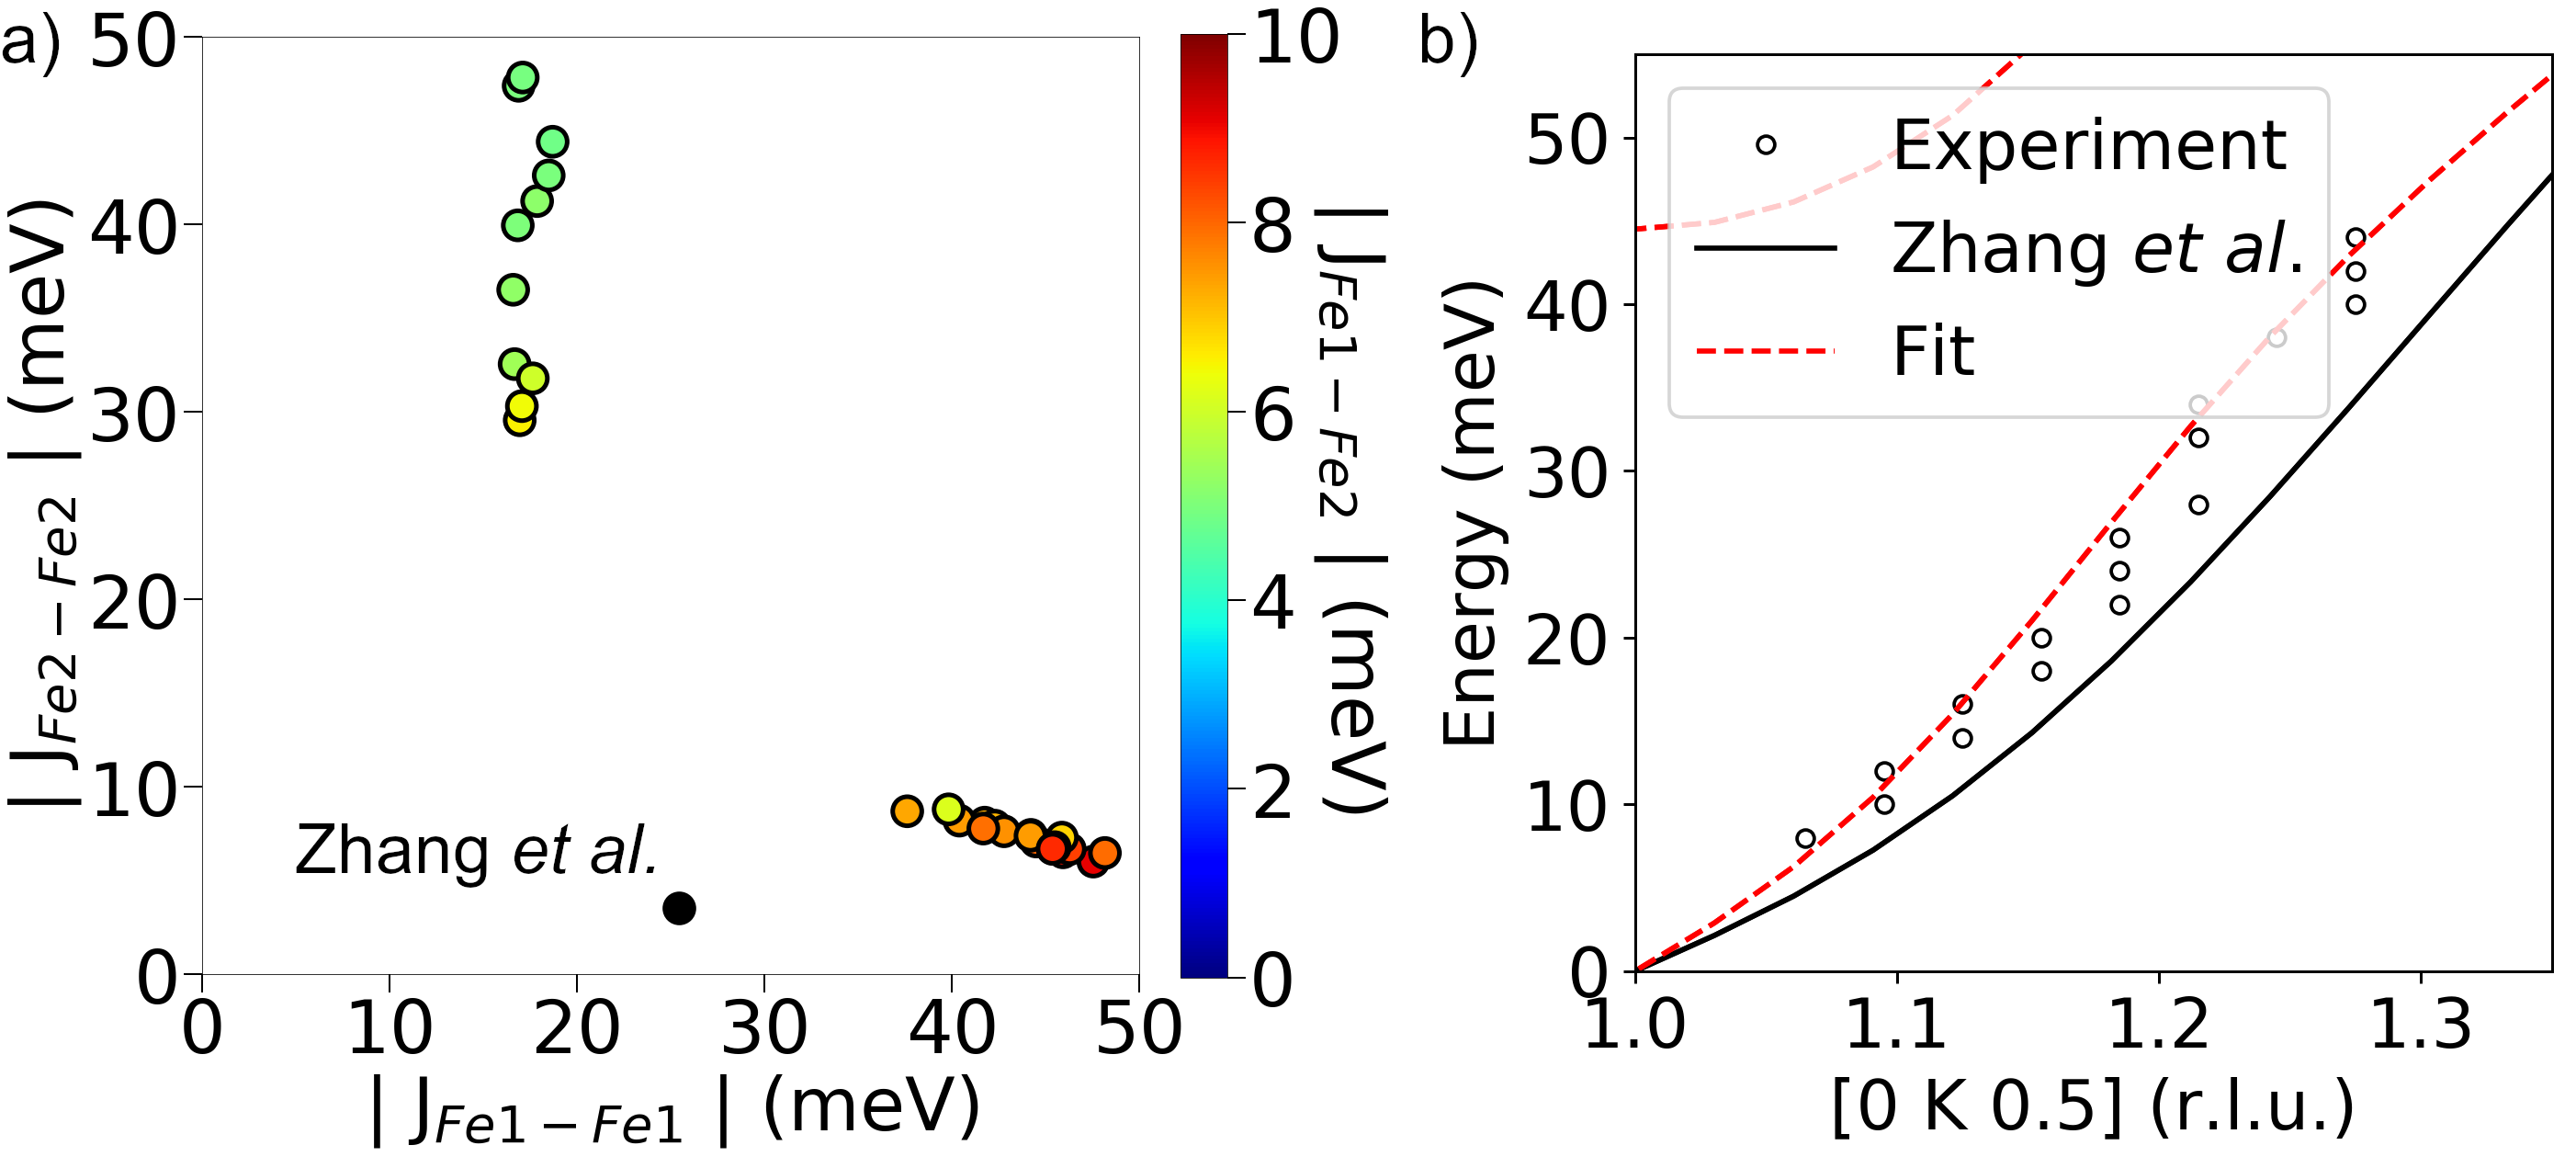
\includegraphics[width=0.8\columnwidth]{figures/ch8/magnon_spectra_refinement.png} \\
\caption{\label{fig:zhang_spinw_refinement}
The result of unconstrained optimization of the exchange coupling values when only three nearest-neighbor interactions are considered is shown in (a). The reduced $\chi^2$ values of all points are less than 7, but these three-$J_{ij}$ fits are disallowed by intensity mismatches to the INS data. In (b), comparison of the fit of a four-$J_{ij}$ model obtained by fixing the NNN Fe2-Fe2 interaction to be $-8.52$~meV and the calculated magnon spectra from the exchange constants from Zhang \emph{et al}. \cite{Zhang2013} leads to an improvement of the fit, with much larger Fe1-Fe1 interaction (see Table \ref{tab:Jvalues}). 
}
\end{figure}

Fe$_2$As is expected to contain a strong Fe1-Fe1 exchange interaction due to a strong anti-bonding interaction as seen in crystal orbital Hamilton population curves \cite{Zhang2013}.
The Fermi level crosses a narrow band along the $X$--$R$ Brillouin zone boundary. Weak Fe2-Fe2 interaction is expected due to the weak antibonding $xy$ and $xz$ orbital overlap at point $R$. However, there is a significant overlap of the Fe2 and As orbitals indicating a possibility of strong superexchange interaction \cite{Zhang2013}. The Fe1-Fe1 and Fe1-Fe2 nearest neighbor exchange interactions can be attributed to direct exchange and the nearest-neighbor and next-nearest-neighbor (NNN) Fe2-Fe2 exchange interactions can be attributed to indirect exchange although there is some direct exchange also possible in the nearest neighbor Fe2-Fe2 exchange interactions \cite{Zhang2013}.  Strong indirect exchange interactions have been reported for MnFeAs, another compound in the Cu$_2$Sb structure type, using SPRKKR calculations \cite{Zhang2015}. From the study of MnFeAs, we can say that there are two possible contributions to the indirect exchange interactions in this material. One effect is due to superexchange interactions mediated by As atoms and the other effect arises from RKKY interactions due to the compound being metallic \cite{Zhang2015}.


The smallest number of exchange coupling constants required to produce magnon modes along $L$ are the Fe1-Fe2 and Fe2-Fe2 nearest-neighbor interactions. However, the fit is poor (reduced $\chi^2$ = 9.03) and is greatly improved upon adding a third $J_{ij}$, the other nearest-neighbor exchange interaction Fe1-Fe1. 
The refinement with three $J_{ij}$ was carried out using the particle swarm optimization technique with a limit of 20 iterations.
Selecting points having reduced $\chi^2 < 7$  from the result of 50 runs, Fig. \ref{fig:zhang_spinw_refinement}(a) shows the exchange constants obtained when the magnon spectra is refined to a model containing only the three nearest-neighbor exchange interactions. 
We can roughly divide the points into two clusters. The cluster of exchange coupling values with strong Fe2-Fe2 nearest-neighbor interactions are incorrect since we know from previous computational studies that Fe$_2$As should have nearest neighbor strong Fe1-Fe1 coupling and a weak Fe2-Fe2 coupling \cite{Zhang2013}. Also, the intensity of the magnon modes in the simulated magnon spectra for this set of $J_{ij}$ arising from [0 1 0.5] is weak, as shown in Fig. \ref{fig:3J_spinw_refinement}(a), which is invalidated by the experimental data. In the other cluster, the Fe1-Fe1 nearest neighbor exchange coupling seems much higher than the reported value of 25.4~meV. However, the simulated magnon spectra from any point in that three-$J_{ij}$ cluster shows that the magnon spectra becomes mostly flat above 60~meV and also drops down below 60~meV near $K = 1$ and 2 as shown in Fig. \ref{fig:3J_spinw_refinement}(b). This is not seen in the experimental magnon spectra. The addition of a fourth $J_{ij}$ is necessary to prevent the magnon spectra from flattening at high energies. Similar to Zhang \emph{et al}. \cite{Zhang2013}, we can choose the NNN Fe2-Fe2 exchange interaction as the fourth exchange interaction for refinement.


The effect of adding a NNN Fe2-Fe2 exchange interaction is mainly at higher energies where the experimental spectra are unresolved. Thus a fourth $J_{ij}$ is necessary, but not refinable from INS data. We fixed the value of the Fe2-Fe2 NNN exchange interaction to that of Zhang \emph{et al}. \cite{Zhang2013} and the remaining three nearest-neighbor exchange interactions were refined 50 times. Four of the runs converged to a reduced $\chi^2 \approx 6.5$, as compared to $\chi^2 > 9$ for the rest of the runs. The mean exchange coupling value from the four runs is shown in Table \ref{tab:Jvalues} and the calculated magnon spectrum using linear spin wave theory is plotted in Fig. \ref{fig:zhang_spinw_refinement}(b). We can see that the Fe1-Fe1 nearest-neighbor exchange interaction is much stronger than the SPRKKR value, which was also seen in the earlier model with only three nearest-neighbor exchange interactions. One should note that, for the sake of optimization, an upper limit of 50~meV was kept for all exchange coupling constants. The value for Fe1-Fe1 exchange coupling is close to this limit. Given that the Fe1-As bond is shorter than one of the Fe2-As bonds, it is possible that there is also some superexchange component in the NNN Fe1-Fe2 interaction. The Fe1-Fe2 distance of 4.4~\AA\ is also shorter than the NNN Fe2-Fe2 distance (4.4716~\AA), allowing for possible RKKY interactions. Although we do not have enough experimental data to elucidate the role of this exchange interaction, it may not be neglected.

If AF materials are to be used in future MRAM devices, it is essential that the 4-fold in-plane anisotropy values surpass 10~meV so that the domains are stable at operating temperatures. Unlike CuMnAs, Fe$_2$As is complicated by the presence of two different magnetic atom sites with different point groups. When the current is parallel to the N\'eel vector, the effective fields on the two Fe sublattices from the field-like torque are perpendicular to each other and the strength of the Fe1-Fe2 exchange interaction may play a role in the electrical switching of the N\'{e}el vector. Hence, it is important that we are able to predict and measure these interactions accurately. Similar to refining the magnon spectra from the experiment, the exchange coupling values obtained from SPRKKR calculations are also contingent on the chosen model. Exchange interactions obtained from ab-initio calculations are known to give largely different values than the experiment, as seen in the case of Mn$_3$Sn \cite{Park2018}. Hence, a more robust determination of exchange energies is warranted. Future efforts could be aided by developing the capability to refine these values while considering magnon intensity quantitatively, and by evaluating metallic antiferromagnets where the higher-energy magnon dispersion is experimentally resolvable. 


\section{Conclusions}

The experimental phonon spectra of Fe$_2$As matches the simulated phonon spectra from DFT calculations very well. The simulated magnon spectra calculated using exchange coupling values from Zhang \emph{et al}. agrees qualitatively with the experimental magnon spectra. The energy values are underestimated by about 20\% along $K$ direction. The anisotropy values were deemed small enough to be neglected for the purpose of refinement and the magnon spectra was refined using a Heisenberg Hamiltonian. For the model used in Zhang \emph{et al}., keeping the value of Fe2-Fe2 nearest neighbor interaction to be a constant, the Fe1-Fe1 nearest neighbor exchange interaction was estimated to be much stronger than previously calculated. 
The in-plane and out-of-plane phonon group velocities are the same order of magnitude, but the magnetic interactions are strongly 2D in nature. This shows that the 2D nature of the magnetism does not arise from weak out-of-plane bonding.

\section{Acknowledgments}

This work was undertaken as part of the Illinois Materials Research Science and Engineering Center, supported by the National Science Foundation MRSEC program under NSF Award No. DMR-1720633. The characterization was carried out in part in the Materials Research Laboratory Central Research Facilities, University of Illinois. This work made use of the Illinois Campus Cluster, a computing resource that is operated by the Illinois Campus Cluster Program (ICCP) in conjunction with the National Center for Supercomputing Applications (NCSA) and which is supported by funds from the University of Illinois at Urbana-Champaign. This research is part of the Blue Waters sustained-petascale computing project, which is supported by the National Science Foundation (Awards No. OCI-0725070 and No. ACI-1238993) and the state of Illinois. Blue Waters is a joint effort of the University of Illinois at Urbana-Champaign and its National Center for Supercomputing Applications. This research used resources of the Spallation Neutron Source, a DOE Office of Science User Facility operated by Oak Ridge National Laboratory, and the Advanced Photon Source, a DOE Office of Science User Facility operated for the DOE Office of Science by Argonne National Laboratory under Contract No. DE-AC02-06CH11357. The authors thank Yan Wu, Huibo Cao and Douglas Abernathy for helpful discussions regarding the experiment.

\section{Supplementary}

Information on T0 chopper used for measurements

The T0 chopper blocks the prompt pulse and additional openings of the Fermi chopper.  For E$_i = 30$, 70 and 200~meV, 90~Hz was used. For E$_i = 300$~meV, 120~Hz was used.
For the 400~K 70~meV run, the T0 chopper was at 60~Hz and provided equivalent performance.

\vspace{2em}

\begin{figure}[h]
\centering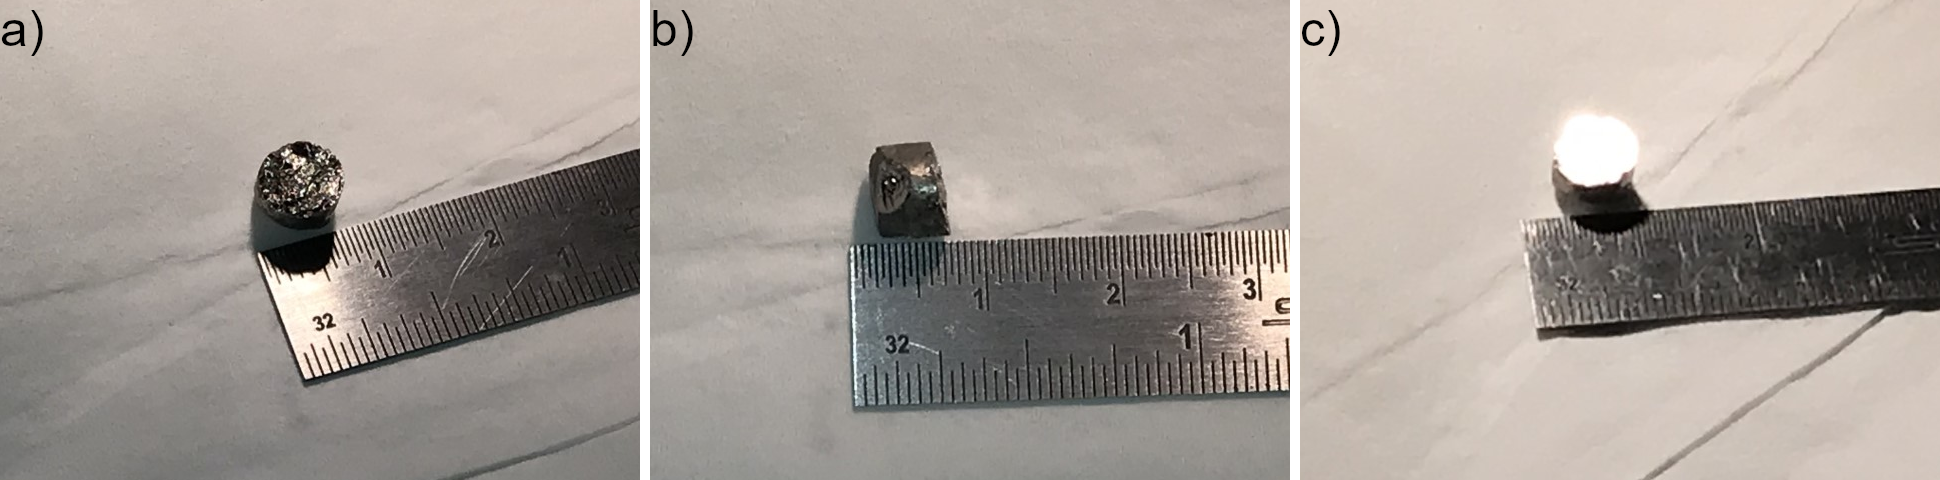
\includegraphics[width=\columnwidth]{figures/ch8/crystal.png} \\
\caption{\label{fig:crystal_array}
One of the Fe$_2$As crystal used for the inelastic neutron scattering measurement with the cleaved surface facing up is shown in (a) and facing to the right side is shown in (b). (c) shows the mirror-like metallic lustre of Fe$_2$As crystals in the cleaved surface when seen from an angle. The values displayed on the scale closest to the sample are in centimeters.
} 
\end{figure}

\begin{figure}[h]
\centering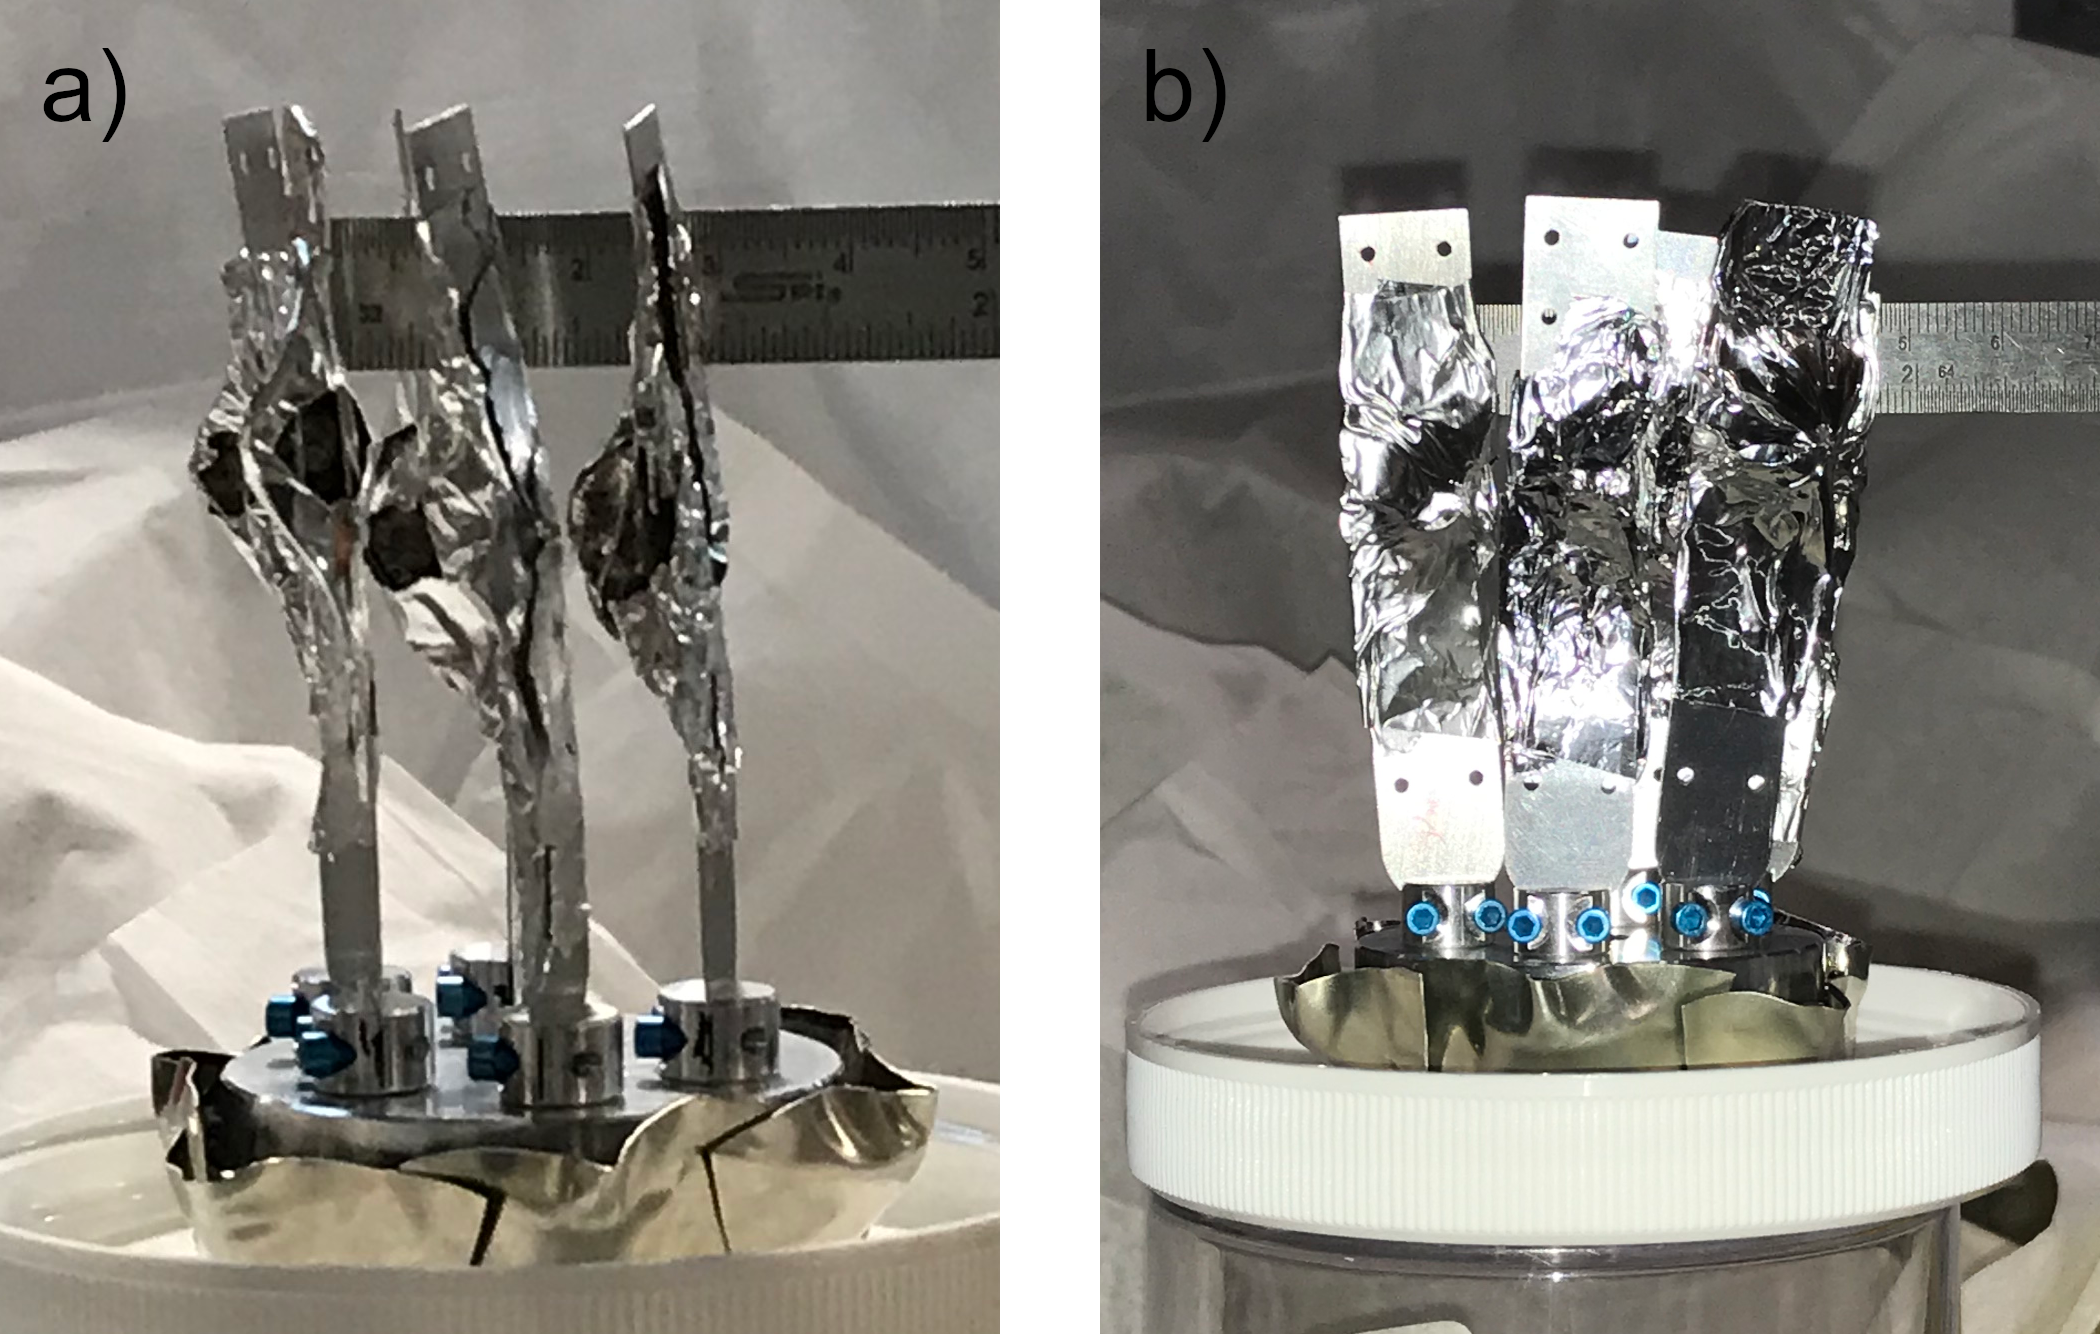
\includegraphics[width=0.5\columnwidth]{figures/ch8/crystal_array.png} \\
\caption{\label{fig:crystal_array}
Five Fe$_2$As single crystals (about 9 g), wrapped in Al foil and co-aligned using the Laue instrument is shown facing (a) $c$ axis of crystal and facing (b) $b$ axis of crystal.
} 
\end{figure}

\begin{figure}[h]
\centering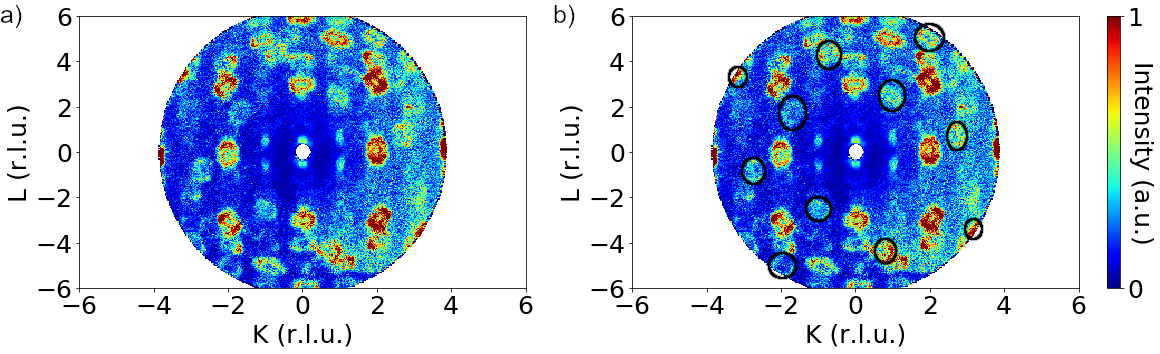
\includegraphics[width=0.8\columnwidth]{figures/ch8/suppl_misaligned_crystal_kl_slice.png} \\
\caption{\label{fig:misaligned_elastic}
A constant energy slice along the $K-L$ plane with energy integrated from 6~meV to 8~meV using $E_i$~=~30 meV is shown in (a). Visible intensity from the misaligned crystal is circled in (b). The misaligned crystal has significant effect on phonons at higher $Q$.
}
\end{figure}


\begin{figure}[h]
\centering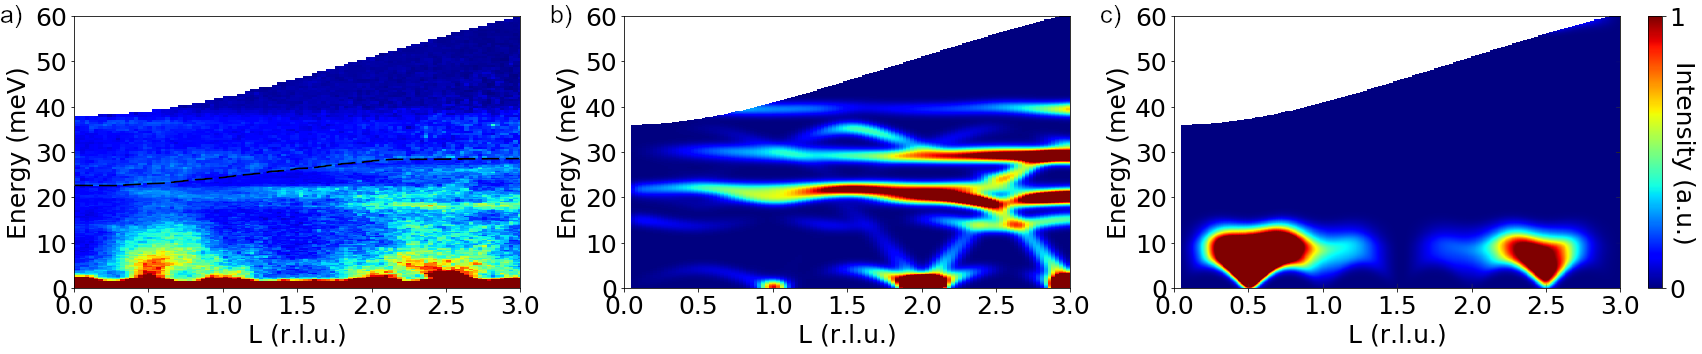
\includegraphics[width=\columnwidth]{figures/ch8/suppl_01L_INS_data.png} \\
\caption{\label{fig:phonon_magnon_spectra_01L}
INS data along $L$ with $H$ integrated from -0.1 to 0.1 and $K$ from -0.9 to 1.1 is shown in (a). Data from E$_i$~=~30~meV (below dashed lines) has been overlaid on top of data from E$_i$~=~70~meV. The corresponding simulated phonon spectra along [0 1 $L$] is shown in (b). (c) shows the magnon spectra along $L$ where $H$ and $K$ have been averaged every 0.025 units in the experimental width.
}
\end{figure}


\begin{figure}[h]
\centering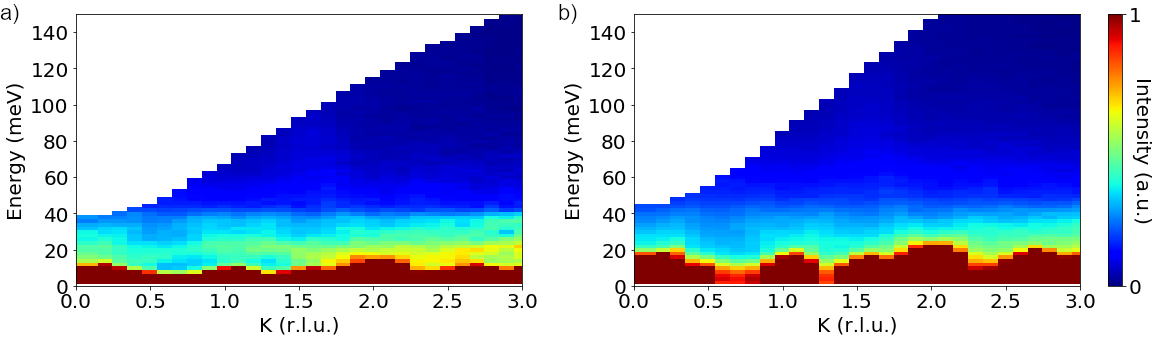
\includegraphics[width=\columnwidth]{figures/ch8/suppl_high_energy_data.png} \\
\caption{\label{fig:high_energy_data}
The magnon spectra along $K$ is shown using $E_i$ = (a) 200~meV and (b) 300~meV where $H$ is integrated from -0.2 to 0.2 and $L$ is integrated from -1 to 1.
}
\end{figure}




\begin{figure}[h]
\centering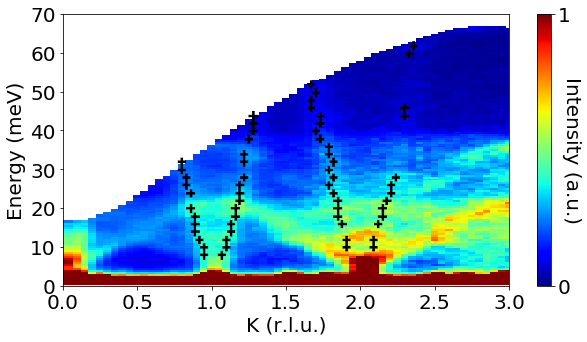
\includegraphics[width=0.6\columnwidth]{figures/ch8/exp_data_points_0K0dot5.png} \\
\caption{\label{fig:exp_data_points_01L}
The experimental data points used for refinement have been overlaid on top of the corresponding magnon spectra along $K$ obtained using $E_i$~=~70~meV. $H$ is integrated from -0.2 to 0.2 and $L$ is integrated from 0.3 to 0.7.
} 
\end{figure}


\begin{figure}[h]
\centering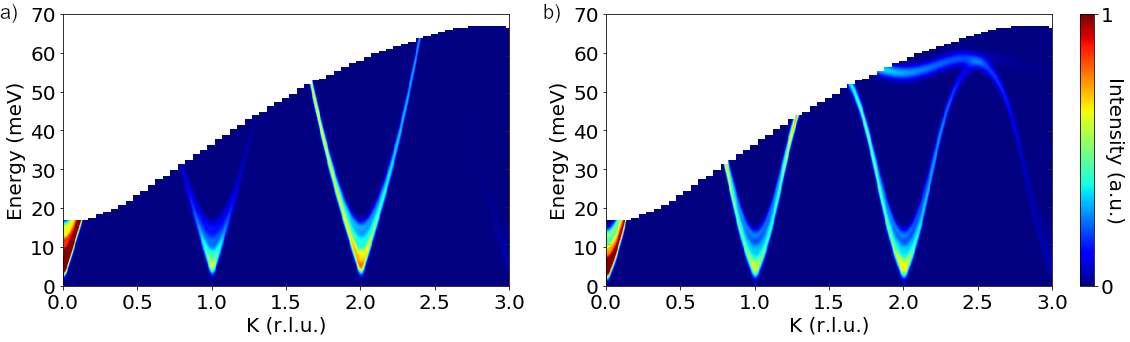
\includegraphics[width=\columnwidth]{figures/ch8/suppl_simulated_magnon_spectra_3J.png} \\
\caption{\label{fig:3J_spinw_refinement}
For a model containing only the three nearest neighbor interactions, the simulated magnon spectra calculated along $K$ with $H$ and $L$ averaged every 0.025 units between 0.0 to 0.1 and 0.5 to 0.6 respectively for (a) a point in the cluster having high Fe2-Fe2 nearest neighbor exchange interaction and low Fe1-Fe1 nearest neighbor exchange interaction and (b) a point in the cluster with small Fe2-Fe2 nearest neighbor exchange interaction but large Fe1-Fe1 nearest neighbor exchange interaction.
}
\end{figure}


%##################chapter 9
\chapter{Conclusions}

\Blindtext[6]

\end{mainmatter}

% }}}

% {{{ back matter

\begin{backmatter}

\bibliographystyle{ieeetr}
\bibliography{thesis}

\end{backmatter}

%\appendix
%\chapter{My Appendix}

%\Blindtext[6]

% }}}

\end{document}
